\documentclass{book}

\usepackage[a4paper,margin=3cm]{geometry}
\usepackage{cite} % for IEEE-style citations
\usepackage{listings}
\usepackage{xcolor}
\usepackage[hidelinks]{hyperref}
\usepackage{graphicx}
\usepackage{setspace}
\usepackage{tcolorbox}
\usepackage[strings]{underscore}
\usepackage{float}
\usepackage[utf8]{inputenc}  
\usepackage{pmboxdraw}

\usepackage{tikz}
\usetikzlibrary{shapes.geometric, arrows.meta, trees, positioning}


\renewcommand{\contentsname}{Daftar Isi}
\renewcommand{\chaptername}{Bab}

% Define Python language style for listings
\lstdefinestyle{PythonStyle}{
    language=Python,
    basicstyle=\ttfamily\footnotesize,
    keywordstyle=\color{blue}\bfseries,
    commentstyle=\color{gray}\itshape,
    stringstyle=\color{red},
    showstringspaces=false,
    breaklines=true,
    frame=lines,
    numbers=left,
    numberstyle=\tiny\color{gray},
    backgroundcolor=\color{lightgray!10},
    tabsize=4,
    captionpos=b
}

\lstdefinestyle{sql}{
	language=sql,
	keywords={use, insert, into, values, select, from,
	update, set, delete, create, where, join, left, right, inner, order, by, primary, key},
	ndkeywords={max, min, varchar, int},
	ndkeywordstyle=\color{purple}\bfseries,
	basicstyle=\ttfamily\footnotesize,
	keywordstyle=\color{blue},
	commentstyle=\color{gray},
	stringstyle=\color{red},
	breaklines=true,
	showstringspaces=false,
	tabsize=2,
	captionpos=b,
	numbers=left,
	numberstyle=\tiny\color{gray},
	frame=lines,
	backgroundcolor=\color{lightgray!10},
	comment=[l]{\#},
	morecomment=[s]{/*}{*/},
	commentstyle=\color{gray}\ttfamily,
	string=[s]{'}{'},
	morestring=[s]{"}{"},
	%	stringstyle=\color{teal}\ttfamily,
	%	showstringspaces=false
}

\lstdefinelanguage{bash} {
	keywords={},
	basicstyle=\ttfamily\small,
	keywordstyle=\color{blue}\bfseries,
	ndkeywords={iex},
	ndkeywordstyle=\color{purple}\bfseries,
	sensitive=true,
	commentstyle=\color{gray},
	stringstyle=\color{red},
	numbers=left,
	numberstyle=\tiny\color{gray},
	breaklines=true,
	frame=lines,
	backgroundcolor=\color{lightgray!10},
	tabsize=2,
	comment=[l]{\#},
	morecomment=[s]{/*}{*/},
	commentstyle=\color{gray}\ttfamily,
	stringstyle=\color{purple}\ttfamily,
	showstringspaces=false,
	captionpos=b
}


\begin{document}
		
	\begin{titlepage}
		\centering
		\vspace*{1cm}
		
		\Huge
		\textbf{IF120203 - Modul Praktikum Pemrograman Dasar}
		
		\vspace{0.5cm}
		
		\LARGE
		Universitas Pradita
		
		\vspace{1.5cm}
		
		\textit{Powered by ChatGPT}
		
		\vspace{2cm}
		
		\textbf{Alfa Yohannis, Ariya Panna}
		
		\vspace{0.8cm}
		
		\today
		
		\vfill
	\end{titlepage}
	
	% Contents Page
	\tableofcontents

	\chapter{Pendahuluan}

\section{Sejarah Pemrograman dan Python}

Pemrograman komputer dimulai pada abad ke-19 dengan penemuan mesin analitik oleh Charles Babbage dan program pertama yang ditulis oleh Ada Lovelace. Sejak itu, pemrograman telah berkembang pesat dengan munculnya bahasa-bahasa pemrograman awal seperti Fortran, COBOL, dan Lisp pada tahun 1950-an. Pada tahun 1970-an dan 1980-an, bahasa pemrograman seperti C, Pascal, dan Basic memperkenalkan konsep-konsep baru dalam pemrograman. Kini, berbagai bahasa pemrograman modern seperti Python, JavaScript, dan Rust digunakan dalam berbagai aplikasi.

Python merupakan bahasa pemrograman \textit{high-level} serbaguna yang pertama kali diperkenalkan pada tahun 1991 oleh Guido van Rossum (GvR). Bahasa ini dirancang agar mudah dipahami dan memiliki struktur kode yang jelas (\textit{readable}), serta mendukung fitur penanganan kesalahan (\textit{exception handling}). Dengan tujuan tersebut, Python berhasil berkembang menjadi bahasa pemrograman yang dapat dimanfaatkan di berbagai bidang. Python merupakan bahasa pemrograman multi-paradigma, yang artinya dapat menggunakan gaya/metode beragam dalam penulisan kode. Saat ini, Python banyak digunakan untuk pengembangan aplikasi web (\textit{server-side}), analisis data, hingga penerapan kecerdasan buatan dan pembelajaran mesin (\textit{machine learning}).
\section{Instalasi di Windows}

Untuk menginstal Python di Windows, ikuti langkah-langkah berikut:

\begin{enumerate}
\item Unduh installer Python terbaru dari situs resmi \href{https://www.python.org/downloads/}{python.org}.
\item Jalankan file installer \texttt{.exe} dan ikuti petunjuk untuk menyelesaikan instalasi.
\item Saat instalasi, centang opsi \textbf{``Add Python to PATH''} agar Python otomatis dikenali di Command Prompt.
\item Ikuti petunjuk instalasi hingga selesai.
\item Verifikasi instalasi dengan membuka Command Prompt lalu ketik:
\begin{verbatim}
    python --version
    pip --version
\end{verbatim}
\end{enumerate}

\section{Instalasi di macOS}

Untuk menginstal Python di macOS, ikuti langkah-langkah berikut:

\begin{enumerate}
\item Unduh installer Python terbaru dari \href{https://www.python.org/downloads/macos/}{python.org}.
\item Jalankan file installer \texttt{.pkg} dan ikuti petunjuk hingga selesai.
\item Alternatif lain, Anda bisa menggunakan Homebrew dengan menjalankan perintah berikut di Terminal:
\begin{verbatim}
    brew install python
\end{verbatim}
\item Setelah instalasi selesai, verifikasi dengan perintah:
\begin{verbatim}
    python3 --version
    pip3 --version
\end{verbatim}
\end{enumerate}

\section{Instalasi di Linux}

Untuk menginstal Python di Linux, ikuti langkah-langkah berikut:

\begin{enumerate}
\item Buka terminal dan jalankan perintah berikut untuk memastikan repositori diperbarui dan Python terpasang:
\begin{verbatim}
    sudo apt update
    sudo apt install python3 python3-pip
\end{verbatim}
\item Verifikasi instalasi dengan perintah:
\begin{verbatim}
    python3 --version
    pip3 --version
\end{verbatim}
\end{enumerate}

\section{IDE dan Editor untuk Python}

\subsection{Apa Itu IDE?}

Integrated Development Environment (IDE) adalah perangkat lunak yang menyediakan fasilitas lengkap untuk pengembangan perangkat lunak. IDE umumnya mencakup editor kode, kompiler atau interpreter, debugger, dan alat manajemen proyek. IDE dirancang untuk mempermudah proses pengembangan perangkat lunak dengan menyediakan antarmuka pengguna yang terintegrasi dan alat-alat yang mendukung pengkodean, pengujian, dan debugging.

Dalam praktikum Python, terdapat beberapa pilihan IDE atau editor yang bisa digunakan, antara lain Visual Studio Code, IDLE (editor bawaan Python), dan PyCharm. Namun, Anda dapat menggunakan IDE atau editor lain yang Anda sukai. Modul praktikum ini menggunakan Visual Studio Code sebagai contoh.

\subsection{Cara Menginstal Visual Studio Code}

\begin{enumerate}
    \item Unduh installer VS Code dari situs resmi \url{https://code.visualstudio.com/}.
    \item Pilih installer sesuai sistem operasi Anda (Windows, macOS, atau Linux).
    \item Jalankan file installer dan ikuti petunjuk instalasi.
    \item Setelah instalasi selesai, buka aplikasi VS Code.
    \item Untuk mendukung pemrograman Python, instal ekstensi \textbf{Python} dari Microsoft melalui menu Extensions (ikon kotak di sidebar kiri).
    \item Untuk membuat file Python, buka menu File (ikon kotak di sidebar kiri) lalu pilih New File (ikon kotak di sidebar kiri) dan ketik nama file yang diinginkan diakhiri dengan \texttt{.py}. Contoh \texttt{hello.py}.
    \item Sekarang Anda dapat mulai menulis dan menjalankan kode Python di dalam VS Code.
\end{enumerate}

\section{Kode Python: hello_world.py}\label{sec:hello_world_code}

\begin{lstlisting}[style=PythonStyle, caption={Kode Python: hello_world.py}]
print("Hello World!")
\end{lstlisting}

Kode di atas merupakan program Python sederhana yang mencetak "Hello World!" ke konsol. Berikut penjelasan dari setiap bagian kode tersebut:

\begin{itemize}
\item \texttt{print(...)} – \texttt{print} adalah fungsi bawaan (\textit{built-in function}) di Python yang digunakan untuk menampilkan output ke layar atau konsol.
\item \texttt{"Hello World!"} – Merupakan sebuah string (teks) yang ditulis di dalam tanda kutip ganda. Nilai string ini akan menjadi argumen yang dikirim ke fungsi \texttt{print}.
\end{itemize}

\section{Panduan Menjalankan Program Python}

Untuk menjalankan program Python di atas, ikuti langkah-langkah berikut:

\begin{enumerate}
	\item Buka terminal atau command prompt.
	\item Navigasikan ke direktori tempat file `hello_world.py` disimpan.
	\begin{verbatim}
		cd /path/ke/direktori
	\end{verbatim}
	\item Jalankan perintah berikut untuk mengkompilasi program:
	\begin{verbatim}
		python hello_world.py
	\end{verbatim}
	\item Jika tidak ada error, program akan dijalankan dan menampilkan "Hello World!" di konsol.
\end{enumerate}

\section{Kode Python: hello_with_input.py}

\begin{lstlisting}[style=PythonStyle, caption={Kode Python: hello_with_input.py}]
nama = input("Masukkan nama Anda: ") # Menerima input dari pengguna

print("Hello " + nama + "!") # Menampilkan output dengan input pengguna
\end{lstlisting}

Berikut penjelasan dari setiap bagian kode tersebut:

\begin{itemize}
\item \texttt{nama = input("Masukkan nama Anda: ")} - Fungsi input merupakan \textit{built-in function} yang digunakan untuk menerima input pengguna dari konsol. Fungsi ini menunda eksekusi program sampai pengguna memasukkan input dan menampilkan opsional pesan untuk meminta input yang kemudian disimpan dalam variabel \texttt{nama}.
\item \texttt{print("Hello " + nama + " !")} - Seperti yang dijelaskan pada Section~\ref{sec:hello_world_code}, fungsi print digunakan untuk mencetak output ke layar atau konsol. Di sini, pesan "Hello [Nama]!" diisi dengan input pengguna.
\end{itemize}


\section{Latihan}

Berikut adalah beberapa latihan yang dapat Anda coba untuk memperdalam pemahaman tentang program Python yang telah dibahas:

\begin{enumerate}
\item \label{sec:first-exercise} \textbf{Latihan 1:} Buat file baru dengan nama \textbf{introduction.py} yang dimana program harus menerima input nama, usia, dan domisili dari pengguna kemudian mencetak pesan dengan format yang ditentukan
\begin{lstlisting}[style=PythonStyle, caption={Latihan 1}]
nama = input("Masukkan nama Anda: ")
prodi = input("Masukkan program studi Anda: ")
angkatan = input("Masukkan angkatan Anda: ")

print("Halo! Nama saya " + nama + ". Saya mahasiswa program studi " + prodi + " tahun angkatan " + angkatan + ".")
\end{lstlisting}

Contoh input dan output yang diberikan ketika program dijalankan:

\begin{verbatim}
Input:
Masukkan Nama Anda: Bob Smith
Masukkan Program Studi Anda: Informatika
Masukkan Tahun Angkatan: 2025

Output:
Halo! Nama saya Bob Smith. Saya mahasiswa program studi Informatika tahun angkatan 2025.
\end{verbatim}

\item \textbf{Latihan 2:} Latihan ini bertujuan untuk belajar memformat teks (\textit{string}) menggunakan \textbf{f-string}, membuat output lebih rapi tanpa perlu menggunakan operator \texttt{+} sebagai penghubung antara teks. Buat file baru dengan nama \textbf{introduction_with_fstring.py} dan isinya mirip dengan \hyperref[sec:first-exercise]{Latihan 1}, namun format outputnya menggunakan \textbf{f-string}

\begin{lstlisting}[style=PythonStyle, caption={Latihan 2}]
nama = input("Masukkan nama Anda: ")
prodi = input("Masukkan program studi Anda: ")
angkatan = input("Masukkan angkatan Anda: ")

print(f"Halo! Nama saya {nama}. Saya mahasiswa program studi {prodi} tahun angkatan {angkatan}. Output dihasilkan menggunakan f-string")
\end{lstlisting}

Contoh input dan output yang diberikan ketika program dijalankan:

\begin{verbatim}
Input:
Masukkan Nama Anda: Bob Smith
Masukkan Program Studi Anda: Informatika
Masukkan Tahun Angkatan: 2025

Output:
Halo! Nama saya Bob Smith. Saya mahasiswa program studi Informatika tahun angkatan 2025. 
Output dihasilkan menggunakan f-string
\end{verbatim}

\item \textbf{Latihan 3:} \textit{Escape Character} merupakan karakter khusus yang digunakan (biasanya diawali dengan \texttt{\textbackslash}) yang digunakan di dalam string untuk mengatur penataan teks atau menampilkan karakter spesial. Dengan escape character, kita bisa:

\begin{itemize}
    \item Membuat teks pindah baris: \texttt{\textbackslash n}
    \item Menambahkan tabulasi: \texttt{\textbackslash t}
    \item Menulis tanda kutip di dalam string: \texttt{\textbackslash "}
    \item Menampilkan backslash asli: \texttt{\textbackslash\textbackslash}
\end{itemize}

Buat file baru dengan nama \textbf{escape_character.py} dan isinya seperti berikut:

\begin{lstlisting}[style=PythonStyle, caption={Latihan 3}]
print("Hello\nWorld") # Membuat teks pindah baris
print("Hello\tWorld") # Menambahkan tabulasi
print("Hello \"World") # Menulis tanda kutip di dalam string
print("Hello \\ World") # Menampilkan backslash asli
\end{lstlisting}

Output yang akan dihasilkan dari program di atas adalah:

\begin{verbatim}
Hello
World
Hello	World
Hello "World
Hello \ World
\end{verbatim}
\end{enumerate}

\section{Soal Latihan}

Berikut adalah beberapa soal latihan tambahan untuk menguji pemahaman Anda mengenai konsep yang telah dipelajari:

\begin{enumerate}
\item \textbf{Soal 1:} Buat program bernama \texttt{biodata.py} yang meminta input berupa:
\begin{itemize}
	\item Nama lengkap
	\item Umur
	\item Hobi
\end{itemize}
	Cetak output dengan format berikut menggunakan \textbf{f-string}. Berikut merupakan contoh input dan output yang diharapkan:
\begin{verbatim}
Input:
Masukkan Nama Lengkap: Jane Hopkins
Masukkan Usia Anda: 20
Masukkan Hobi Anda: Ngoding

Output:
Halo, nama saya Jane Hopkins. Saya berusia 20 tahun dan hobi saya adalah Ngoding.
\end{verbatim}

\item \textbf{Soal 2:}  
Buat program bernama \texttt{quote.py} yang menampilkan kutipan favoritmu. Gunakan \textbf{escape character} untuk menampilkan tanda kutip di dalam string. Contoh output:

\begin{verbatim}
Input:
Masukkan kutipan favoritmu dari Albert Einstein: "Imagination is more important 
than knowledge."

Output:
Kata Albert Einstein: "Imagination is more important than knowledge."
\end{verbatim}

\item \textbf{Soal 3:} Buat program bernama \texttt{schedule.py} yang menampilkan jadwal kuliah. Gunakan \textbf{tabulasi} (\texttt{\textbackslash t}) untuk merapikan kolom. Contoh output:

\begin{tabular}{l l l}
    \textbf{Hari} & \textbf{Waktu} & \textbf{Mata Kuliah} \\
    Senin & 07.00 & Algoritma \\
    Selasa & 09.00 & Basis Data \\
    Selasa & 13.00 & Pemrograman Dasar \\
\end{tabular}
\end{enumerate}

	\chapter{Variabel, Konstanta, Tipe Data Dasar, dan Konversi Tipe Data}

\section{Variabel}

Variabel merupakan tempat penyimpanan sementara yang digunakan untuk menampung data selama program berjalan, sehingga data tersebut dapat digunakan kembali. Berbeda dengan bahasa pemrograman \textit{static type} seperti C, C++, dan Java yang harus secara eksplisit menulis tipe data untuk variabel. Di Python, variabel memiliki tipe data yang dinamis (\textit{dynamic type}) dan dapat berubah sesuai dengan kebutuhan program.
\newline

\begin{figure}[H]
	\centering
	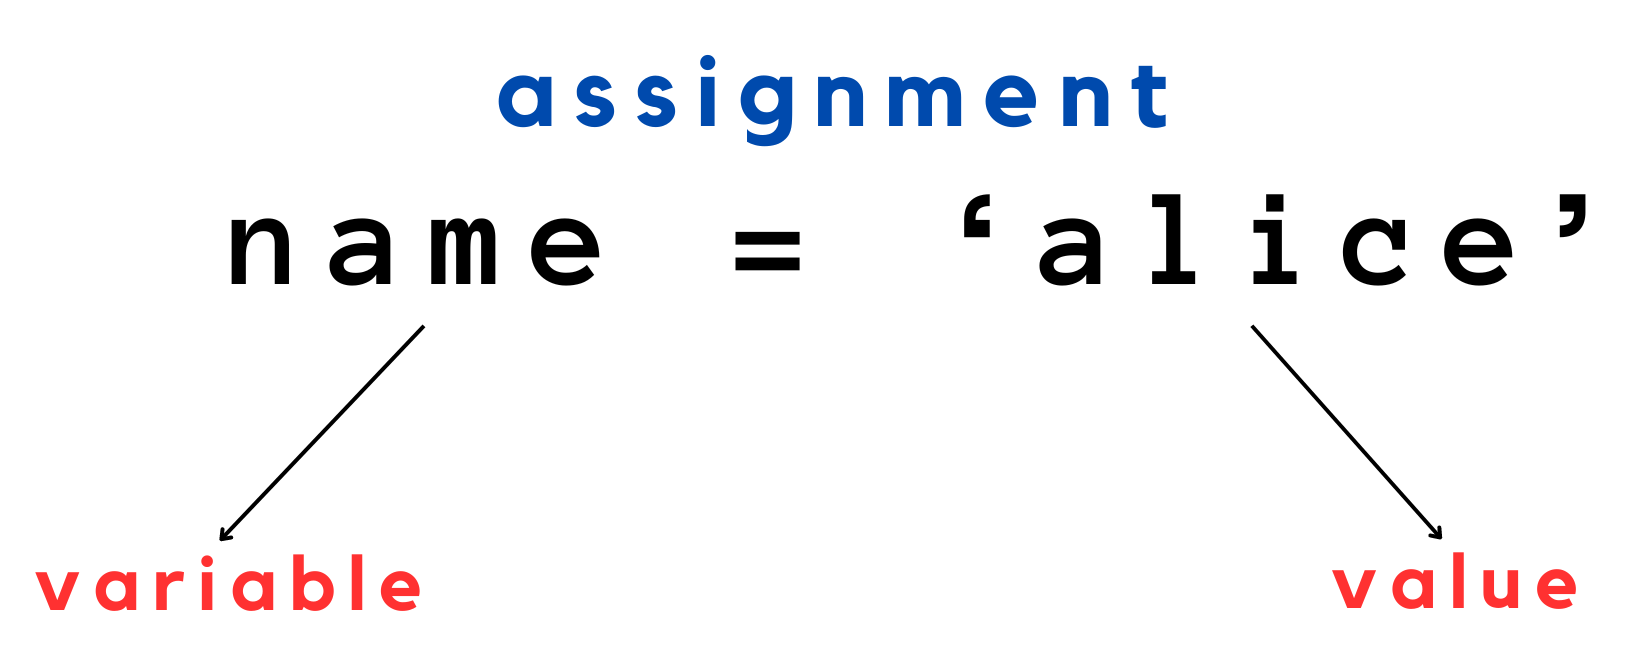
\includegraphics[width=0.7\textwidth]{../shared_assets/images/python_variable_structure.png}
	\caption{Struktur Variabel di Python}
	\label{fig:python-variable-structure}
\end{figure}

\noindent
Sumber gambar: \url{https://www.packetswitch.co.uk/python-variables-data-types/}

\subsection{Aturan Penamaan Variabel}

Pemberian nama variabel di Python harus mematuhi beberapa aturan penamaan yang disediakan oleh Python. Berikut adalah beberapa aturan penamaan variabel di Python:

\begin{itemize}
	\item Nama variabel harus dimulai dengan huruf atau underscore (\_).
	\item Nama variabel tidak boleh dimulai dengan angka.
	\item Nama variabel tidak boleh mengandung spasi.
	\item Nama variabel tidak boleh mengandung simbol.
	\item Nama variabel tidak boleh mengandung kata kunci (\textit{keyword}) yang sudah terdefinisi dalam Python, seperti \texttt{def}, \texttt{for}, \texttt{if}, \texttt{return}, dan sebagainya.
\end{itemize}

\subsection{Latihan Membuat Variabel}

Buat file baru dengan nama \textbf{variable.py} dan buat variabel dengan nama \textbf{nama}, \textbf{usia}, dan \textbf{berat_badan} dengan tipe data yang sesuai dan nilai-nilai yang sesuai. Kemudian cetak variabel tersebut.

\begin{lstlisting}[style=PythonStyle, caption={Kode Python: variable.py}]
nama = "Stefani Laurensia"
usia = 21
berat_badan = 50.2

print(nama)
print(usia)
print(berat_badan)
\end{lstlisting}

\subsection{Contoh Kesalahan Penamaan Variabel}

\begin{lstlisting}[style=PythonStyle, caption={Kode Python: variable.py}]
1angka = 200 # Nama variabel tidak boleh dimulai dengan angka
nama lengkap = "Budi" # Nama variabel tidak boleh mengandung spasi
gaji$ = 1000000 # Nama variabel tidak boleh mengandung simbol
class = "Informatika" # class merupakan kata kunci untuk membuat sebuah class di Python sehingga melanggar aturan di mana nama variabel tidak boleh mengandung kata kunci
\end{lstlisting}

\section{Konstanta}

Konstanta adalah variabel yang seharusnya nilainya tidak berubah selama program berjalan. Contohnya nilai \textbf{\textit{pi}} (3.14) atau gravitasi (9.81). Di Python, kita bisa menandai variabel sebagai Final dari modul \texttt{typing} untuk memberi tanda bahwa variabel tersebut dimaksudkan sebagai konstanta. Namun ada hal-hal yang perlu diperhatikan:
\begin{itemize}
	\item Python tidak memaksa variabel \texttt{Final} agar tidak bisa diubah.
	\item Penandaan \texttt{Final} hanya \textbf{memberi peringatan pada type checker}, bukan mencegah perubahan di runtime.
\end{itemize}

\subsection{Aturan Penamaan Konstanta}

Untuk menandakan bahwa sebuah variabel adalah konstanta, kita bisa menggunakan huruf besar untuk membedakan dengan variabel biasa. Hal ini mengikuti aturan penamaan variabel yang dibuat oleh Python (\href{https://peps.python.org/pep-0008/}{PEP 8 - Style Guide for Python Code}).

\subsection{Latihan Membuat Konstanta}

Buat file baru dengan nama \textbf{constant.py} dan buat konstanta dengan nama \textbf{PI} dan \textbf{GRAVITASI} dengan nilai yang sesuai. Kemudian cetak konstanta tersebut. Namun, berbeda dari bahasa pemrograman lain seperti C, C++, atau Java, di Python konstanta dapat diubah.
\begin{lstlisting}[style=PythonStyle, caption={Kode Python: constant.py}]
from typing import Final

PI: Final = 3.14
GRAVITASI: Final = 9.81

print(PI)
print(GRAVITASI)

GRAVITASI = 10 # Nilai masih tetap bisa berubah, tapi tidak disarankan
print(GRAVITASI)
\end{lstlisting}

\section{Tipe Data Dasar}

Tipe data merupakan jenis data yang bisa disimpan di program Python. Tipe data di Python memiliki banyak jenis, seperti \texttt{int}, \texttt{float}, \texttt{str}, \texttt{bool}, \texttt{list}, \texttt{tuple}, \texttt{dict}, dan \texttt{set}. Namun pada \textit{chapter} kali ini, kita akan fokus pada tipe data dasar, antara lain \texttt{int}, \texttt{float}, \texttt{str}, dan \texttt{bool}.
\newline \newline
Berdasarkan kelompoknya, tipe data dasar di Python dapat dibedakan menjadi 3 kelompok, antara lain:

\begin{enumerate}
\item \textbf{Numeric} (Angka)
\begin{enumerate}
\item \textbf{Integer} (bilangan bulat)
\begin{lstlisting}[style=PythonStyle]
usia = 18
jumlah_mahasiswa = 64
nomor_rumah = 88

suhu = -5
\end{lstlisting}

\item \textbf{Float} (bilangan desimal)
\begin{lstlisting}[style=PythonStyle]
koordinat_x = 5.5
koordinat_y = 7.8

saldo = 10.500.075
\end{lstlisting}
\end{enumerate}

\item \textbf{Teks} (Kata / Kalimat)
\begin{enumerate}
\item \textbf{String} (kumpulan karakter)
\begin{lstlisting}[style=PythonStyle]
nama = "John"
quote = 'Programmer: A machine that turns coffee into code'
pesan_email = """
Kepada Yth. John Doe,

Terima kasih atas pesanan anda.
"""
\end{lstlisting}
\end{enumerate}

\item \textbf{Boolean} (Benar atau Salah)
\begin{lstlisting}[style=PythonStyle]
is_married = False
is_single = True
\end{lstlisting}
\end{enumerate}

\section{Konversi Tipe Data (\textit{Type Casting})}

Kadang kita perlu mengubah tipe data dari satu jenis ke jenis lain agar Python bisa memprosesnya dengan benar.
Misal, input dari pengguna melalui fungsi \texttt{input()} selalu mengembalikan tipe data string (str), tapi kita ingin melakukan perhitungan angka, maka kita harus mengubahnya menjadi int atau float.

\begin{table}[h!]
\centering
\begin{tabular}{|c|c|c|}
\hline
\textbf{Fungsi} & \textbf{Keterangan} & \textbf{Contoh} \\
\hline
int() & Ubah menjadi bilangan bulat & int("10") → 10 \\
\hline
float() & Ubah menjadi bilangan desimal & float("3.14") → 3.14 \\
\hline
str() & Ubah menjadi teks & str(10) → "10" \\
\hline
bool() & Ubah menjadi True/False & bool(0) → False, bool(5) → True \\
\hline
\end{tabular}
\caption{Fungsi Untuk Konversi Tipe Data di Python}
\end{table}

\subsection{Latihan Konversi Tipe Data}

\begin{lstlisting}[style=PythonStyle, caption={Kode Python: string_to_int.py}]
usia = input("Masukkan usia Anda: ")
print("Tipe data sebelum konversi:", type(usia)) # Menampilkan tipe data sebelum konversi

usia = int(usia) # Konversi tipe data string menjadi integer
print("Tipe data setelah konversi:", type(usia)) # Menampilkan tipe data setelah konversi

usia_lima_tahun_kemudian = usia + 5 # Perhitungan usia 5 tahun kemudian
print("Usia 5 tahun kemudian:", usia_lima_tahun_kemudian)
\end{lstlisting}

\begin{lstlisting}[style=PythonStyle, caption={Kode Python: string_to_float.py}]
angka_str = "45.67"
print("Sebelum konversi:", angka_str, type(angka_str))

angka_float = float(angka_str)
print("Setelah konversi ke float:", angka_float, type(angka_float))
\end{lstlisting}

\begin{lstlisting}[style=PythonStyle, caption={Kode Python: int_to_float.py}]
angka_int = 10
print("Sebelum konversi:", angka_int, type(angka_int))

angka_float = float(angka_int)
print("Setelah konversi ke float:", angka_float, type(angka_float))
\end{lstlisting}

\begin{lstlisting}[style=PythonStyle, caption={Kode Python: float_to_int.py}]
angka_float = 3.99
print("Sebelum konversi:", angka_float, type(angka_float))

angka_int = int(angka_float)
print("Setelah konversi ke integer:", angka_int, type(angka_int))
\end{lstlisting}

\subsection{Kesalahan dalam Konversi Tipe Data}
Meskipun Python menyediakan fungsi bawaan untuk mengubah tipe data (\texttt{int()}, \texttt{float()}, \texttt{str()}, \texttt{bool()}), \textbf{tidak semua konversi bisa dilakukan dengan sukses}. Jika nilai yang dikonversi tidak sesuai dengan tipe data tujuan, maka program akan menghasilkan \textbf{error}. Berikut adalah contoh kesalahan dalam konversi tipe data:

\begin{lstlisting}[style=PythonStyle]
# String huruf → Integer
huruf = "abc"
huruf_integer = int(huruf) 
# Output: ValueError: invalid literal for int() with base 10: 'abc'

# String bilangan desimal → Integer
angka_str = "12.34"
angka_int = int(angka_str)  
# Output: ValueError: invalid literal for int() with base 10: '12.34'
\end{lstlisting}

Perhatikan pada contoh di atas bahwa program akan menghasilkan \textbf{error} ketika nilai yang dikonversi tidak sesuai dengan tipe data tujuan. Hal ini diakibatkan karena fungsi \texttt{int()} hanya dapat mengubah \textbf{string yang berisi bilangan bulat} menjadi tipe data \texttt{integer}.
\par
Apabila string berisi karakter non-angka (misalnya \texttt{"abc"}) atau bilangan desimal (misalnya \texttt{"12.34"}), maka Python tidak dapat memprosesnya langsung sebagai \texttt{integer} dan akan menampilkan pesan \texttt{ValueError}. Untuk kasus bilangan desimal dalam bentuk string, diperlukan dua tahap konversi, yaitu:
\begin{enumerate}
	\item Konversi string ke tipe data \texttt{float}.
	\item Konversi tipe data \texttt{float} ke tipe data \texttt{integer}.
\end{enumerate}

\section{Soal Latihan}

Berikut adalah beberapa soal latihan tambahan untuk menguji pemahaman Anda mengenai konsep variabel, konstanta tipe data, dan konversi tipe data yang telah dipelajari:
\begin{enumerate}
\item \textbf{Soal 1:} Buat program bernama \texttt{luas_persegi_panjang.py} yang meminta pengguna memasukan nilai panjang dan lebar persegi panjang, kemudian program harus bisa menghitung dan mencetak luas persegi panjang tersebut.
\newline \newline
\textbf{Hint:} Gunakan operator perkalian \texttt{*} untuk menghitung luas.

\item \textbf{Soal 2:} Buat program bernama \texttt{luas_lingkaran.py} yang meminta pengguna memasukan nilai jari-jari lingkaran. Program harus menampung nilai konstanta \textbf{\textit{pi}} mengikuti standar \textit{best practice} dari Python dan bisa menghitung sekaligus mencetak luas lingkaran tersebut.

\item \textbf{Soal 3:} Buat program bernama \texttt{tebak_usia.py} yang meminta pengguna memasukkan tahun lahirnya. Program harus:
\begin{enumerate}
    \item Menyimpan tahun lahir di variabel.
    \item Mengubah input dari string menjadi integer.
    \item Menghitung umur dengan mengurangi tahun saat ini dengan tahun lahir yang dimasukan oleh pengguna.
    \item Menampilkan pesan seperti: "Kamu berusia [umur] tahun."
\end{enumerate}

\textbf{Hint:} Gunakan operator pengurangan \texttt{-} untuk menghitung usia saat ini.

\end{enumerate}
	\chapter{Operator dan Pengkondisian}

\section{Operator}
Operator adalah karakter khusus yang digunakan untuk melakukan operasi terhadap variabel dan nilai. Di Python terdapat berbagai jenis operator, namun pada chapter ini kita hanya akan membahas beberapa operator yang paling umum digunakan, yaitu:

\begin{enumerate}
    \item Operator Aritmatika
    \item Operator \textit{Assignment}
    \item Operator Perbandingan
    \item Operator Logika
    \item Operator \textit{Membership}
\end{enumerate}

\subsection{Operator Aritmatika}
\begin{frame}[fragile]{Operator Aritmatika di Python}
Operator ini dipakai untuk melakukan operasi dasar dalam matematika, seperti penjumlahan, pengurangan, perkalian, pembagian, dan sebagainya.

\end{frame}

\begin{table}[H]
\centering
\begin{tabular}{|c|c|c|}
\hline
\textbf{Operator} & \textbf{Keterangan} \\
\hline
\texttt{+} & Operator penjumlahan \\
\hline
\texttt{-} & Operator pengurangan \\
\hline
\texttt{*} & Operator perkalian \\
\hline
\texttt{/} & Operator pembagian \\
\hline
\texttt{//} & Operator pembagian bulat (\textit{floor division}) \\
\hline
\texttt{\%} & Operator modulus (sisa hasil bagi) \\
\hline
\texttt{**} & Operator perpangkatan \\
\hline
\end{tabular}
\caption{Daftar Operator Aritmatika di Python}
\end{table}

Berikut adalah contoh penggunaan operator aritmatika dalam Python:
\begin{lstlisting}[style=PythonStyle, caption={Kode Python: arithmetic_operator.py}]
a = 5
b = 2

print("a + b =", a + b)
print("a - b =", a - b)
print("a * b =", a * b)
print("a / b =", a / b)
print("a // b =", a // b)
print("a % b =", a % b)
print("a ** b =", a ** b)
\end{lstlisting}

Kode di atas mendemonstrasikan berbagai operasi aritmatika yang dapat dilakukan di Python menggunakan operator bawaan. Berikut adalah penjelasan dari setiap operasi:
\begin{itemize}
    \item Penjumlahan (+)
    \begin{itemize}
        \item \texttt{print("a + b =", a + b)} menghasilkan penjumlahan dari \texttt{a} dan \texttt{b}, yaitu $5 + 2 = 7$.
    \end{itemize}

    \item Pengurangan (-)
    \begin{itemize}
        \item \texttt{print("a - b =", a - b)} menghasilkan pengurangan dari \texttt{a} dan \texttt{b}, yaitu $5 - 2 = 3$.
    \end{itemize}

    \item Perkalian (*)
    \begin{itemize}
        \item \texttt{print("a * b =", a * b)} menghasilkan perkalian dari \texttt{a} dan \texttt{b}, yaitu $5 \times 2 = 10$.
    \end{itemize}

    \item Pembagian (/)
    \begin{itemize}
        \item \texttt{print("a / b =", a / b)} menghasilkan pembagian dari \texttt{a} dan \texttt{b}, yaitu $5 / 2 = 2.5$.
    \end{itemize}

    \item \textit{Floor Division} (//)
    \begin{itemize}
        \item \texttt{print("a // b =", a // b)} menghasilkan pembagian bulat dari \texttt{a} dan \texttt{b} dengan pembulatan ke bawah, yaitu $5 // 2 = 2$.
    \end{itemize}

    \item Modulo (\%)
    \begin{itemize}
        \item \texttt{print("a \% b =", a \% b)} menghasilkan sisa hasil bagi dari \texttt{a} dibagi \texttt{b}, yaitu $5 \% 2 = 1$.
    \end{itemize}

    \item Perpangkatan (**)
    \begin{itemize}
        \item \texttt{print("a ** b =", a ** b)} menghasilkan \texttt{a} dipangkatkan dengan \texttt{b}, yaitu $5^2 = 25$.
    \end{itemize}
\end{itemize}

\subsection{Operator \textit{Assignment}}
Operator \textit{assignment} adalah operator yang digunakan untuk memberikan nilai pada variabel. 
Selain \textit{assignment} dasar dengan tanda sama dengan (\texttt{=}), Python juga menyediakan operator 
\textit{assignment} gabungan (\textit{augmented assignment}) yang mengombinasikan operasi aritmatika dengan assignment.

\begin{table}[H]
\centering
\begin{tabular}{|c|c|}
\hline
\textbf{Operator} & \textbf{Keterangan} \\
\hline
\texttt{=} & Assignment, memberikan nilai ke variabel \\
\hline
\texttt{+=} & Penjumlahan sekaligus assignment (\texttt{x += y} $\Rightarrow$ \texttt{x = x + y}) \\
\hline
\texttt{-=} & Pengurangan sekaligus assignment (\texttt{x -= y} $\Rightarrow$ \texttt{x = x - y}) \\
\hline
\texttt{*=} & Perkalian sekaligus assignment (\texttt{x *= y} $\Rightarrow$ \texttt{x = x * y}) \\
\hline
\texttt{/=} & Pembagian sekaligus assignment (\texttt{x /= y} $\Rightarrow$ \texttt{x = x / y}) \\
\hline
\texttt{//=} & Floor division sekaligus assignment (\texttt{x //= y} $\Rightarrow$ \texttt{x = x // y}) \\
\hline
\texttt{\%=} & Modulo sekaligus assignment (\texttt{x \%= y} $\Rightarrow$ \texttt{x = x \% y}) \\
\hline
\texttt{**=} & Perpangkatan sekaligus assignment (\texttt{x **= y} $\Rightarrow$ \texttt{x = x ** y}) \\
\hline
\end{tabular}
\caption{Daftar Operator Assignment di Python}
\end{table}

Berikut adalah contoh penggunaan operator assignment dalam Python:
\begin{lstlisting}[style=PythonStyle, caption={Kode Python: assignment_operator.py}]
x = 10
print("x =", x)

x += 5
print("x += 5 ->", x)

x -= 3
print("x -= 3 ->", x)

x *= 2
print("x *= 2 ->", x)

x /= 4
print("x /= 4 ->", x)

x //= 2
print("x //= 2 ->", x)

x %= 3
print("x %= 3 ->", x)

x **= 2
print("x **= 2 ->", x)
\end{lstlisting}

Kode di atas mendemonstrasikan berbagai operator assignment yang dapat digunakan di Python. 
Berikut adalah penjelasan dari setiap operator:
\begin{itemize}
    \item Assignment (=)
    \begin{itemize}
        \item \texttt{x = 10} memberikan nilai $10$ ke variabel \texttt{x}.
    \end{itemize}

    \item Penjumlahan Assignment (+=)
    \begin{itemize}
        \item \texttt{x += 5} sama dengan \texttt{x = x + 5}. Jika sebelumnya $x = 10$, maka setelah operasi ini $x = 15$.
    \end{itemize}

    \item Pengurangan Assignment (-=)
    \begin{itemize}
        \item \texttt{x -= 3} sama dengan \texttt{x = x - 3}. Jika $x = 15$, maka hasilnya $x = 12$.
    \end{itemize}

    \item Perkalian Assignment (*=)
    \begin{itemize}
        \item \texttt{x *= 2} sama dengan \texttt{x = x * 2}. Jika $x = 12$, maka hasilnya $x = 24$.
    \end{itemize}

    \item Pembagian Assignment (/=)
    \begin{itemize}
        \item \texttt{x /= 4} sama dengan \texttt{x = x / 4}. Jika $x = 24$, maka hasilnya $x = 6.0$.
    \end{itemize}

    \item Floor Division Assignment (//=)
    \begin{itemize}
        \item \texttt{x //= 2} sama dengan \texttt{x = x // 2}. Jika $x = 6.0$, maka hasilnya $x = 3.0$.
    \end{itemize}

    \item Modulo Assignment (\%=)
    \begin{itemize}
        \item \texttt{x \%= 3} sama dengan \texttt{x = x \% 3}. Jika $x = 3.0$, maka hasilnya $x = 0.0$.
    \end{itemize}

    \item Perpangkatan Assignment (**=)
    \begin{itemize}
        \item \texttt{x **= 2} sama dengan \texttt{x = x ** 2}. Jika $x = 0.0$, maka hasilnya tetap $0.0$.
    \end{itemize}
\end{itemize}

\subsection{Operator Perbandingan}
Operator perbandingan digunakan untuk membandingkan dua nilai. 
Hasil dari operator ini selalu berupa nilai boolean (\texttt{True} atau \texttt{False}).

\begin{table}[H]
\centering
\begin{tabular}{|c|c|}
\hline
\textbf{Operator} & \textbf{Keterangan} \\
\hline
\texttt{==} & Sama dengan \\
\hline
\texttt{!=} & Tidak sama dengan \\
\hline
\texttt{>} & Lebih besar dari \\
\hline
\texttt{<} & Lebih kecil dari \\
\hline
\texttt{>=} & Lebih besar atau sama dengan \\
\hline
\texttt{<=} & Lebih kecil atau sama dengan \\
\hline
\end{tabular}
\caption{Daftar Operator Perbandingan di Python}
\end{table}

\begin{lstlisting}[style=PythonStyle, caption={Kode Python: comparison_operator.py}]
a = 5
b = 2

print("a == b:", a == b)
print("a != b:", a != b)
print("a > b:", a > b)
print("a < b:", a < b)
print("a >= b:", a >= b)
print("a <= b:", a <= b)
\end{lstlisting}

\subsection{Operator Logika}
Operator logika digunakan untuk menggabungkan ekspresi boolean.

\begin{table}[H]
\centering
\begin{tabular}{|c|c|}
\hline
\textbf{Operator} & \textbf{Keterangan} \\
\hline
\texttt{and} & Bernilai \texttt{True} jika kedua kondisi bernilai benar \\
\hline
\texttt{or} & Bernilai \texttt{True} jika salah satu kondisi bernilai benar \\
\hline
\texttt{not} & Membalikkan nilai boolean (True menjadi False, sebaliknya) \\
\hline
\end{tabular}
\caption{Daftar Operator Logika di Python}
\end{table}

\begin{lstlisting}[style=PythonStyle, caption={Kode Python: logical_operator.py}]
x = True
y = False

print("x and y:", x and y)
print("x or y:", x or y)
print("not x:", not x)
\end{lstlisting}

\subsection{Operator \textit{Membership}}
Operator \textit{membership} digunakan untuk memeriksa apakah suatu nilai (biasanya berupa karakter atau substring) 
terdapat di dalam sebuah string. Hasil dari operasi ini berupa nilai boolean (\texttt{True} atau \texttt{False}).

\begin{table}[H]
\centering
\begin{tabular}{|c|c|}
\hline
\textbf{Operator} & \textbf{Keterangan} \\
\hline
\texttt{in} & Bernilai \texttt{True} jika nilai ada di dalam string \\
\hline
\texttt{not in} & Bernilai \texttt{True} jika nilai tidak ada di dalam string \\
\hline
\end{tabular}
\caption{Daftar Operator \textit{Membership} di Python}
\end{table}

\begin{lstlisting}[style=PythonStyle, caption={Kode Python: membership_operator.py}]
text = "Python Programming"

print("'Py' in text:", "Py" in text)         # True
print("'Java' in text:", "Java" in text)     # False
print("'Java' not in text:", "Java" not in text) # True
print("'P' in text:", "P" in text)           # True
\end{lstlisting}

\section{Pengkondisian}
Pengkondisian adalah konsep penting dalam pemrograman yang memungkinkan pengambilan keputusan berdasarkan kondisi tertentu. Di Python, pengkondisian bisa diimplementasikan menggunakan beberapa struktur dasar seperti if, elif, else, match, dan operator ternary.

\subsection{If}
If digunakan untuk mengeksekusi blok kode tertentu hanya jika kondisi yang diberikan bernilai true. Bentuk dasarnya adalah:

\begin{lstlisting}[style=PythonStyle, caption={Bentuk dasar if}]
if kondisi:
    # Blok kode yang akan dieksekusi jika kondisi bernilai true
\end{lstlisting}

Contoh Penggunaan:

\begin{lstlisting}[style=PythonStyle, caption={Kode Python: if_statement.py}]
nilai = 75
if nilai >= 70:
    print("Lulus")
\end{lstlisting}

\subsection{If-Else}
If-else memungkinkan kita untuk menentukan blok kode alternatif yang akan dijalankan jika kondisi tidak terpenuhi. Bentuk dasarnya adalah:

\begin{lstlisting}[style=PythonStyle, caption={Bentuk dasar if-else}]
if kondisi:
    # Blok kode yang akan dieksekusi jika kondisi bernilai true
else:
    # Blok kode yang akan dieksekusi jika kondisi bernilai false
\end{lstlisting}

Contoh Penggunaan:

\begin{lstlisting}[style=PythonStyle, caption={Kode Python: if_else_statement.py}]
nilai = 65
if nilai >= 70:
    print("Lulus")
else:
    print("Tidak Lulus")
\end{lstlisting}

\subsection{If-Elif-Else (Percabangan Multi Kondisi)}
If-elif-else memungkinkan kita untuk menentukan beberapa kondisi dan blok kode yang akan dijalankan jika kondisi tersebut bernilai true. Bentuk dasarnya adalah:

\begin{lstlisting}[style=PythonStyle, caption={Bentuk dasar if-elif-else}]
if kondisi1:
    # Blok kode yang akan dieksekusi jika kondisi1 bernilai true
elif kondisi2:
    # Blok kode yang akan dieksekusi jika kondisi2 bernilai true
else:
    # Blok kode yang akan dieksekusi jika kondisi1 dan kondisi2 bernilai false
\end{lstlisting}

Contoh Penggunaan:

\begin{lstlisting}[style=PythonStyle, caption={Kode Python: if_elif_else_statement.py}]
nilai = 65
if nilai >= 90:
    print("A")
elif nilai >= 80:
    print("B")
elif nilai >= 70:
    print("C")
else:
    print("D")
\end{lstlisting}

\subsection{\textit{Nested-If}}
\textit{Nested-if} adalah struktur if yang digunakan untuk membuat blok kode yang bersarang. Bentuk dasarnya adalah:

\begin{lstlisting}[style=PythonStyle, caption={Bentuk dasar nested-if}]
if kondisi1:
    # Blok kode yang akan dieksekusi jika kondisi1 bernilai true
    if kondisi2:
        # Blok kode yang akan dieksekusi jika kondisi2 bernilai true
    else:
        # Blok kode yang akan dieksekusi jika kondisi2 bernilai false
else:
    # Blok kode yang akan dieksekusi jika kondisi1 bernilai false
\end{lstlisting}

Contoh Penggunaan:

\begin{lstlisting}[style=PythonStyle, caption={Kode Python: nested_if_statement.py}]
usia = 25
punya_surat_izin_mengemudi = True

if usia >= 18:  # Kondisi luar: cek apakah usia sudah 18 tahun ke atas
    print("Kamu sudah dewasa.")
    if punya_surat_izin_mengemudi:  # Kondisi dalam: cek apakah sudah punya SIM
        print("Kamu boleh mengemudi.")
    else:
        print("Kamu sudah dewasa, tapi belum punya SIM.")
else:
    print("Kamu belum dewasa.")
\end{lstlisting}

\subsection{\textit{Match}}
Sejak Python 3.10, tersedia struktur kontrol baru bernama \texttt{match} yang mirip dengan \texttt{switch-case} di bahasa pemrograman lain. Dengan \texttt{match}, kita dapat mencocokkan sebuah nilai terhadap beberapa pola sekaligus. Bentuk dasarnya adalah:

\begin{lstlisting}[style=PythonStyle, caption={Bentuk dasar match}]
match variabel / value:
    case pola1:
        # blok kode jika sesuai pola1
    case pola2:
        # blok kode jika sesuai pola2
    case _:
        # blok kode default jika tidak ada yang cocok
\end{lstlisting}

Berikut contoh penggunaannya:

\begin{lstlisting}[style=PythonStyle, caption={Kode Python: match.py}]
hari = "Senin"

match hari:
    case "Senin":
        print("Awal minggu, semangat kerja!")
    case "Jumat":
        print("Akhir minggu, hampir libur!")
    case _:
        print("Hari biasa.")
\end{lstlisting}

\subsection{Operator Ternary (\textit{Conditional Expression})}

Python mendukung bentuk singkat dari struktur \texttt{if-else} yang disebut dengan
\textit{conditional expression} atau sering dikenal sebagai \textit{ternary operator}.
Sintaksnya adalah:

\begin{lstlisting}[style=PythonStyle, caption={Bentuk dasar ternary operator di Python}]
nilai_jika_true if kondisi else nilai_jika_false
\end{lstlisting}

Contoh penggunaannya:

\begin{lstlisting}[style=PythonStyle, caption={Kode Python: ternary_operator.py}]
usia = 20

status = "Dewasa" if usia >= 18 else "Anak-anak"

print("Status:", status)
\end{lstlisting}

Kode di atas setara dengan:

\begin{lstlisting}[style=PythonStyle]
if usia >= 18:
    status = "Dewasa"
else:
    status = "Anak-anak"
\end{lstlisting}

\section{Latihan}
Berikut adalah beberapa latihan yang dapat Anda coba untuk memperdalam pemahaman tentang program Python yang telah dibahas:

\begin{enumerate}
\item \textbf{Latihan 1:} Buatlah program yang menerima input 5 nilai asesmen mahasiswa yang kemudian dihitung rata-ratanya. Berdasarkan rata-rata tersebut buatlah pengkondisian menggunakan \textit{if-elif-else statement} untuk menentukan grade yang sesuai dengan ketentuan:
\begin{itemize}
    \item Grade A jika rata-rata berada di \textit{range} 90,00 - 100
    \item Grade A- jika rata-rata berada di \textit{range} 85,00 - 89,99
    \item Grade B+ jika rata-rata berada di \textit{range} 80,00 - 84,99
    \item Grade B jika rata-rata berada di \textit{range} 75,00 - 79,99
    \item Grade B- jika rata-rata berada di \textit{range} 70,00 - 74,99
    \item Grade C+ jika rata-rata berada di \textit{range} 65,00 - 69,99
    \item Grade C jika rata-rata berada di \textit{range} 60,00 - 64,99
    \item Grade D jika rata-rata berada di \textit{range} 55,00 - 59,99
    \item Grade E jika rata-rata kurang dari 49,99
\end{itemize}

\item \textbf{Latihan 2:} Buatlah program untuk menghitung \textit{Body Mass Index} (BMI) seseorang dengan rumus:

\[
BMI = \frac{berat \ (kg)}{(tinggi \ (m))^2}
\]

\begin{itemize}
    \item Program meminta input berat badan (kg) dan tinggi badan (cm).
    \item Konversikan tinggi badan dari cm menjadi meter.
    \item Hitung nilai BMI menggunakan rumus di atas.
    \item Kategorikan hasilnya dengan \texttt{if-elif-else}:
    \begin{itemize}
        \item $<$ 18.5 : \texttt{Kurus}
        \item 18.5 -- 24.9 : \texttt{Normal}
        \item 25 -- 29.9 : \texttt{Overweight}
        \item $\geq$ 30 : \texttt{Obesitas}
    \end{itemize}
\end{itemize}

\item \textbf{Latihan 3:} Modifikasi program BMI pada Latihan 2 dengan ketentuan berikut:
\begin{itemize}
    \item Program tetap meminta input berat badan (kg) dan tinggi badan (cm).
    \item Konversikan tinggi badan dari cm ke meter, lalu hitung nilai BMI.
    \item Gunakan struktur \texttt{if-elif-else} untuk menentukan kategori BMI:
    \begin{itemize}
        \item $<$ 18.5 : \texttt{"kurus"}
        \item 18.5 -- 24.9 : \texttt{"normal"}
        \item 25 -- 29.9 : \texttt{"overweight"}
        \item $\geq$ 30 : \texttt{"obesitas"}
    \end{itemize}
    \item Setelah kategori ditentukan, gunakan \texttt{match-case} untuk menampilkan pesan sesuai kategori:
    \begin{itemize}
        \item \texttt{"kurus"} : tampilkan pesan untuk memperhatikan asupan gizi
        \item \texttt{"normal"} : tampilkan pesan untuk mempertahankan pola hidup sehat
        \item \texttt{"overweight"} : tampilkan pesan untuk mulai menjaga pola makan
        \item \texttt{"obesitas"} : tampilkan pesan untuk konsultasi ke dokter
    \end{itemize}
\end{itemize}


\item \textbf{Latihan 4:} Buatlah program autentikasi sederhana yang meminta pengguna untuk memasukkan email dan password. Program harus memenuhi kriteria sebagai berikut:
\begin{itemize}
    \item Email harus berupa alamat email dengan domain \texttt{pradita.ac.id}
    \item Password harus memiliki panjang minimal 8 karakter
    \item Gunakan \textit{data dummy} (statis), misalnya email \texttt{mahasiswa@pradita.ac.id} dan password \texttt{password123}, untuk proses pencocokan
\end{itemize}

\item \textbf{Latihan 5:} Buatlah program kalkulator sederhana yang:
\begin{itemize}
    \item Meminta pengguna memilih operasi aritmatika yang ingin dilakukan (\texttt{+}, \texttt{-}, \texttt{*}, \texttt{/})
    \item Meminta pengguna memasukkan dua buah angka
    \item Menampilkan hasil perhitungan sesuai operasi yang dipilih
    \item Jika pengguna memasukkan operasi yang tidak valid, tampilkan pesan error
\end{itemize}

\end{enumerate}
	\chapter{Fungsi and Modul}

\section{Fungsi}
Fungsi adalah blok kode terorganisir yang memiliki nama tertentu dan dapat dipanggil berulang kali untuk melakukan tugas spesifik, mengurangi redundansi kode, dan mempermudah pengelolaan program. Fungsi membantu kita menulis kode yang lebih rapi, modular, dan mudah dipelihara.

\subsection{Fungsi Dasar Tanpa Parameter}

Fungsi sederhana yang tidak menerima parameter dan tidak mengembalikan nilai. Fungsi ini hanya menjalankan perintah tertentu.

\begin{lstlisting}[style=PythonStyle, caption={Kode Python: basic_function.py}]
def greet():
    print("Halo, selamat datang!")

# Memanggil fungsi
greet()
\end{lstlisting}

\subsection{Fungsi dengan Parameter}

Fungsi bisa memiliki parameter. Dengan adanya parameter, suatu nilai bisa di-sisipkan ke dalam fungsi secara dinamis saat pemanggilannya.

Parameter sendiri merupakan istilah untuk variabel yang menempel pada fungsi, yang mengharuskan kita untuk menyisipkan nilai pada parameter tersebut saat pemanggilan fungsi.

\begin{lstlisting}[style=PythonStyle, caption={Kode Python: parameter_function.py}]
def greet_with_name(nama):
    print(f"Halo, {nama}!")

# Memanggil fungsi dengan argumen
greet_with_name("Jessie")
\end{lstlisting}

\subsection{Fungsi dengan Nilai Kembalian (Return Value)}

Fungsi dapat mengembalikan hasil yang dapat disimpan atau digunakan dalam perhitungan lain.

\subsubsection{Return Nilai Tunggal}
\begin{lstlisting}[style=PythonStyle, caption={Kode Python: function_with_single_return.py}]
def add(a, b):
    return a + b

summation_result = add(5, 3)
print(summation_result)  # Output: 8
\end{lstlisting}

\subsubsection{Return Lebih dari Satu Nilai}
\begin{lstlisting}[style=PythonStyle, caption={Kode Python: function_with_multiple_return.py}]
def operate(a, b):
    return a + b, a * b

sum_result, product_result = operate(4, 5)
print(sum_result)     # 9
print(product_result) # 20
\end{lstlisting}

\subsection{Fungsi dengan Parameter Default}

Fungsi dapat memiliki nilai default untuk parameter jika argumen tidak diberikan saat pemanggilan.

\begin{lstlisting}[style=PythonStyle, caption={Kode Python: function_with_default_parameter.py}]
def greet_you(name="Friend"):
    print(f"Hello, {name}!")

greet_you()        # Output: Hello, Friend!
greet_you("Andrew")  # Output: Hello, Andrew!
\end{lstlisting}

\subsection{Fungsi dengan Argumen Keyword dan Positional}
Fungsi di Python bisa dipanggil menggunakan positional arguments atau keyword arguments. Positional argument adalah istilah untuk urutan parameter/argument fungsi. Pengisian argument saat pemanggilan fungsi harus urut sesuai dengan deklarasi parameternya. Keyword argument atau named argument adalah metode pengisian argument pemanggilan fungsi disertai nama parameter yang ditulis secara jelas (eksplisit).

\begin{lstlisting}[style=PythonStyle, caption={Kode Python: function_with_keyword_and_positional.py}]
def student_info(name, age, major):
    print(f"{name}, {age} years old, majoring in {major}")

# Positional arguments
student_info("Delta", 20, "Computer Science")

# Keyword arguments
student_info(major="Information Systems", name="Echo", age=21)
\end{lstlisting}

\subsection{Fungsi dengan Jumlah Argumen Variabel}

Jika jumlah argumen tidak pasti, kita bisa menggunakan \texttt{*args}.

\begin{lstlisting}[style=PythonStyle, caption={Kode Python: function_with_variable_arguments.py}]
def sum_numbers(*numbers):
    total = sum(numbers)
    print(f"Total: {total}")

sum_numbers(1, 2, 3, 4)  # Output: Total: 10
sum_numbers(5, 6, 7)     # Output: Total: 18
\end{lstlisting}

\subsection{Fungsi Rekursif}

Fungsi yang memanggil dirinya sendiri. Biasanya digunakan untuk masalah yang dapat dipecah menjadi sub-masalah.

\begin{lstlisting}[style=PythonStyle, caption={Kode Python: recursive_function.py}]
def factorial(n):
    if n == 0 or n == 1:
        return 1
    else:
        return n * factorial(n-1)

print(factorial(5))  # Output: 120
\end{lstlisting}

\section{Modul}

Modul adalah file Python (\texttt{.py}) yang berisi kode seperti fungsi, variabel, atau kelas, yang bisa digunakan kembali di program lain. Modul membantu memecah program menjadi bagian-bagian yang lebih kecil dan terstruktur.

\subsection{Membuat Modul}

Modul sendiri dibuat dengan membuat file Python baru. Misalnya kita buat file \texttt{math_operations.py}:

\begin{lstlisting}[style=PythonStyle, caption={Kode Python: math_operations.py}]
def add(a, b):
    """Mengembalikan hasil penjumlahan a + b"""
    return a + b

def subtract(a, b):
    """Mengembalikan hasil pengurangan a - b"""
    return a - b

def multiply(a, b):
    """Mengembalikan hasil perkalian a * b"""
    return a * b

def divide(a, b):
    """Mengembalikan hasil pembagian a / b"""
    if b == 0:
        return "Error: Division by zero!"
    return a / b

def power(a, b):
    """Mengembalikan hasil a pangkat b"""
    return a ** b
\end{lstlisting}

Lalu kita bisa menggunakan modul ini di file program lain:

\begin{lstlisting}[style=PythonStyle, caption={Kode Python: calculator.py}]
import math_operations

print(math_operations.add(5, 3))        # Output: 8
print(math_operations.subtract(10, 4))  # Output: 6
print(math_operations.multiply(2, 7))   # Output: 14
print(math_operations.divide(10, 2))    # Output: 5.0
print(math_operations.power(3, 4))      # Output: 81
\end{lstlisting}

\subsection{Mengimpor Modul dengan Alias}

Kita bisa memberi nama alias saat mengimpor modul agar lebih ringkas:

\begin{lstlisting}[style=PythonStyle, caption={Kode Python: calculator.py}]
import math_operations as mo

print(mo.add(5, 3))        # Output: 8
print(mo.subtract(10, 4))  # Output: 6
print(mo.multiply(2, 7))   # Output: 14
print(mo.divide(10, 2))    # Output: 5.0
print(mo.power(3, 4))      # Output: 81
\end{lstlisting}

\subsection{Menaruh Modul dalam Folder}

Selain membuat modul di satu file, kita juga bisa menaruh modul di dalam folder supaya lebih rapi. Misalnya:

\begin{verbatim}
project/
│
├── main.py
└── utils/
└── string_utils.py
\end{verbatim}

Isi \texttt{string_utils.py} misalnya:

\begin{lstlisting}[style=PythonStyle, caption={Kode Python: utils/string_utils.py}]
def to_upper(text):
return text.upper()

def to_lower(text):
return text.lower()
\end{lstlisting}

Di \texttt{main.py}, kita bisa mengimpor modul ini dari folder \texttt{utils}:

\begin{lstlisting}[style=PythonStyle, caption={Kode Python: main.py}]
from utils import string_utils

print(string_utils.to_upper("Python")) # Output: PYTHON
print(string_utils.to_lower("Python")) # Output: python
\end{lstlisting}

\subsection{Best Practice: Paket dengan __init__.py}

Untuk project yang lebih besar atau modul yang akan digunakan di banyak file, sebaiknya folder modul dijadikan \textbf{package} dengan menambahkan file __init__.py:

\begin{verbatim}
project/
│
├── main.py
└── utils/
├── __init__.py
└── string_utils.py
\end{verbatim}

Dengan __init__.py, Python mengenali folder sebagai package.

Cara import tetap sama:

\begin{lstlisting}[style=PythonStyle]
from utils import string_utils
\end{lstlisting}

\subsubsection{Modul Bawaan Python}

Python memiliki banyak modul bawaan yang bisa langsung digunakan tanpa instalasi. Beberapa modul bawaan yang sering dipakai antara lain:

\texttt{math} — untuk operasi matematika, seperti akar, pangkat, atau konstanta \(\pi\).

\texttt{random} — untuk menghasilkan angka acak.

\texttt{datetime} — untuk mengelola tanggal dan waktu.

\texttt{os} — untuk berinteraksi dengan sistem operasi, misal folder, file, path.

Contoh penggunaan modul bawaan:

\begin{lstlisting}[style=PythonStyle, caption={Kode Python: math_module.py}]
import math

print(math.sqrt(16)) # Output: 4.0
print(math.pi) # Output: 3.141592653589793
\end{lstlisting}

\begin{lstlisting}[style=PythonStyle, caption={Kode Python: random_module.py}]
import random

print(random.randint(1, 10)) # Output: angka acak antara 1 sampai 10
\end{lstlisting}

\begin{lstlisting}[style=PythonStyle, caption={Kode Python: datetime_module.py}]
from datetime import date

today = date.today()
print(today) # Output: tanggal hari ini, misal 2025-09-20
\end{lstlisting}

\subsubsection{Mengimpor Fungsi atau Variabel Tertentu}

Jika hanya membutuhkan beberapa fungsi/variabel dari modul, bisa langsung diimpor:

\begin{lstlisting}[style=PythonStyle]
from math import sqrt, pi

print(sqrt(36)) # Output: 6.0
print(pi) # Output: 3.141592653589793
\end{lstlisting}

\section{Latihan}

\begin{enumerate}
    \item \textbf{Soal 1:} Buatlah program yang meminta pengguna memasukan nilai (minimal 5 input), kemudian klasifikasikan nilai tersebut sesuai dengan ketentuan berikut:
    \begin{enumerate}
        \item Jika nilai lebih besar atau sama dengan 80, maka klasifikasi \texttt{A}
        \item Jika nilai lebih besar atau sama dengan 70, maka klasifikasi \texttt{B}
        \item Jika nilai lebih besar atau sama dengan 60, maka klasifikasi \texttt{C}
        \item Jika nilai lebih besar atau sama dengan 50, maka klasifikasi \texttt{D}
        \item Jika nilai lebih kecil dari 50, maka klasifikasi \texttt{E}
    \end{enumerate}
    Buatkan program dalam dua versi, yaitu dengan membuat fungsi untuk klasifikasi dan tanpa membuat fungsi klasifikasi.

    \item \textbf{Soal 2:} Buatlah program yang meminta pengguna memasukan nilai 3 mata pelajaran (Matematika, Fisika, dan Kimia), kemudian buatlah fungsi yang menerima dua parameter yakni nilai dan parameter kedua nilai minimal kelulusan dengan default nilai 60. Program akan menampilkan lulus atau tidak lulus sesuai dengan nilai minimal. Standar kelulusan untuk matematika adalah 80, untuk fisika adalah 70, dan untuk kimia adalah 60.

    \item \textbf{Soal 3:} Buatlah program untuk menghitung deret Fibonacci dengan cara:
    \begin{enumerate}
        \item Meminta input jumlah angka n dari pengguna
        \item Menggunakan fungsi rekursif untuk menghitung angka Fibonacci ke-n.
        \item Menampilkan deret Fibonacci hingga n angka pertama
    \end{enumerate}

    \item \textbf{Soal 4:} Buat modul bernama \textbf{geometry.py} yang berisi fungsi:
    \begin{enumerate}
        \item \texttt{hitung_persegi_panjang(panjang, lebar)} → mengembalikan luas dan keliling persegi panjang (function with multiple returns)
        \item \texttt{hitung_persegi(sisi)} → mengembalikan luas dan keliling persegi (function with multiple returns)
    \end{enumerate}
    Kemudian import modul tersebut di file program utama dan gunakan fungsi-fungsi tersebut.

\end{enumerate}
	\chapter{Perulangan (Looping)}

\section{Perulangan di Python}
Dalam pemrograman, seringkali kita perlu menjalankan blok kode yang sama berulang kali. 
Misalnya, mencetak angka dari 1 sampai 100, membaca setiap baris dari sebuah file, atau 
memproses setiap elemen dalam sebuah daftar data. 
Proses pengulangan eksekusi blok kode ini dikenal sebagai \textbf{perulangan} atau \textit{looping} (iterasi).

Python menyediakan dua mekanisme utama untuk melakukan perulangan:
\begin{enumerate}
    \item \textbf{Perulangan \texttt{for}}: Digunakan untuk melakukan iterasi pada sebuah urutan (seperti \texttt{list}, \texttt{tuple}, \texttt{string}) atau objek \textit{iterable} lainnya. Perulangan ini sering disebut sebagai \textit{definite iteration} karena jumlah pengulangannya sudah ditentukan oleh panjang urutan.
    \item \textbf{Perulangan \texttt{while}}: Digunakan untuk mengulang blok kode selama sebuah kondisi bernilai \texttt{True}. Perulangan ini disebut \textit{indefinite iteration} karena jumlah pengulangannya tidak pasti dan bergantung pada kapan kondisi menjadi \texttt{False}.
\end{enumerate}

Menguasai perulangan adalah langkah fundamental untuk menulis program yang efisien dan otomatis.

\subsection{For Loop}

Perulangan \texttt{for} di Python bekerja dengan cara mengambil setiap elemen dari sebuah urutan secara bergantian.

\subsection{Sintaks Dasar}
Sintaks umum dari perulangan \texttt{for} adalah sebagai berikut:
\begin{lstlisting}[style=PythonStyle, caption={Sintaks Dasar Perulangan for}]
for nama_variabel in urutan:
    # Blok kode yang akan diulang
    # ...
\end{lstlisting}

\subsection{Iterasi Menggunakan \texttt{range()}}
Fungsi \texttt{range()} sangat umum digunakan bersama \texttt{for} untuk menghasilkan urutan angka.
\begin{itemize}
    \item \texttt{range(stop)}: Membuat urutan dari 0 hingga \texttt{stop-1}.
    \item \texttt{range(start, stop)}: Membuat urutan dari \texttt{start} hingga \texttt{stop-1}.
    \item \texttt{range(start, stop, step)}: Membuat urutan dari \texttt{start} hingga \texttt{stop-1} dengan lompatan sebesar \texttt{step}.
\end{itemize}

\begin{lstlisting}[style=PythonStyle, caption={Kode Python: for_with_range.py}]
# Mencetak angka dari 0 sampai 4
print("Contoh 1: range(5)")
for i in range(5):
    print(f"Perulangan ke-{i}")

# Mencetak angka dari 2 sampai 5
print("\nContoh 2: range(2, 6)")
for j in range(2, 6):
    print(f"Angka: {j}")
\end{lstlisting}

\subsection{Iterasi pada List dan String}
Anda bisa melakukan iterasi secara langsung pada elemen-elemen dari sebuah \texttt{list} atau karakter-karakter dari sebuah \texttt{string}.

\begin{lstlisting}[style=PythonStyle, caption={Kode Python: list_and_string_iteration.py}]
# Iterasi pada sebuah list
daftar_buah = ["apel", "mangga", "jeruk"]
for buah in daftar_buah:
    print(f"Saya suka {buah}")

# Iterasi pada sebuah string
nama = "PYTHON"
for huruf in nama:
    print(huruf, end=' ')
\end{lstlisting}

\section{While Loop}
Perulangan \texttt{while} akan terus mengeksekusi blok kode di dalamnya selama kondisi yang diberikan bernilai \texttt{True}.

\subsection{Sintaks Dasar}
\begin{lstlisting}[style=PythonStyle, caption={Sintaks Dasar Perulangan while}]
while kondisi:
    # Blok kode yang akan diulang
    # ...
    # Penting: Harus ada perubahan yang membuat kondisi akhirnya False
\end{lstlisting}

\textbf{Perhatian:} Pastikan di dalam blok \texttt{while} ada sebuah mekanisme (misalnya, inkrementasi variabel) yang pada akhirnya akan mengubah nilai kondisi menjadi \texttt{False}. Jika tidak, program akan masuk ke dalam \textit{infinite loop} atau perulangan tak terbatas.

\subsection{Contoh Penggunaan}
\begin{lstlisting}[style=PythonStyle, caption={Kode Python: while_loop.py}]
# Menghitung dari 1 sampai 5
angka = 1
while angka <= 5:
    print(f"Hitungan: {angka}")
    angka = angka + 1 # atau angka += 1

print("Selesai")
\end{lstlisting}

\begin{lstlisting}[style=PythonStyle, caption={Kode Python: cowok_selalu_salah.py}]
def cewek_nanya():
    print('Cewek: Kamu salah ga?')

def respon_cowok():
    return input('Cowok: ')

def cek_jawaban_cowok(jawaban):
    if jawaban.startswith('iy'):
        return True
    else:
        return False
    
def main():
    while True:
        cewek_nanya()
        jawaban_cowo = respon_cowok()

        if cek_jawaban_cowok(jawaban_cowo):
            break

main()
\end{lstlisting}

\section{Kontrol Alur Perulangan}
Python menyediakan dua statement untuk mengontrol alur eksekusi di dalam perulangan: \texttt{break} dan \texttt{continue}.

\subsection{\texttt{break} Statement}
Statement \texttt{break} digunakan untuk menghentikan paksa (keluar dari) perulangan saat itu juga, bahkan jika kondisi perulangan masih terpenuhi.

\begin{lstlisting}[style=PythonStyle, caption={Kode Python: break_keyword.py}]
# Mencari angka 5 dalam rentang 1-10
for i in range(1, 11):
    print(i, end=' ')
    if i == 5:
        print("\nAngka 5 ditemukan, perulangan dihentikan!")
        break 
\end{lstlisting}

\subsection{\texttt{continue} Statement}
Statement \texttt{continue} digunakan untuk melewati sisa blok kode pada iterasi saat ini dan langsung melanjutkan ke iterasi berikutnya.

\begin{lstlisting}[style=PythonStyle, caption={Kode Python: continue_keyword.py}]
# Mencetak angka ganjil dari 1 sampai 10
for i in range(1, 11):
    if i % 2 == 0: # Jika angka genap
        continue   # Lewati iterasi ini dan lanjut ke angka berikutnya
    print(f"Angka ganjil: {i}")
\end{lstlisting}

\section{Perulangan Bersarang (\textit{Nested Loops})}
\textit{Nested loop} adalah sebuah perulangan yang berada di dalam perulangan lainnya. Perulangan di dalam (\textit{inner loop}) akan menyelesaikan seluruh iterasinya untuk setiap satu iterasi dari perulangan di luar (\textit{outer loop}).

Konsep ini sering digunakan untuk memproses data dalam format dua dimensi, seperti matriks atau tabel.

\begin{lstlisting}[style=PythonStyle, caption={Kode Python: nested_loop.py}]
# Outer loop untuk baris
for i in range(1, 4):  # Baris 1 sampai 3
    # Inner loop untuk kolom
    for j in range(1, 4): # Kolom 1 sampai 3
        print(f"{i}x{j} = {i*j}", end='\t')
    print() # Pindah ke baris baru setelah inner loop selesai
\end{lstlisting}

\section{Latihan Soal}
Kerjakan soal-soal di bawah ini untuk menguji pemahaman Anda.

\begin{enumerate}
    \item \textbf{Faktorial}: Buatlah sebuah program yang meminta pengguna memasukkan sebuah bilangan bulat positif, lalu hitung dan tampilkan nilai faktorial dari bilangan tersebut menggunakan perulangan \texttt{for}. ($n! = n \times (n-1) \times \dots \times 1$).
    
    \item \textbf{Tebak Angka}: Buatlah sebuah permainan tebak angka sederhana. Program akan memilih sebuah angka acak antara 1 dan 50. Pengguna diminta menebak angka tersebut. Gunakan perulangan \texttt{while} untuk terus meminta input dari pengguna hingga tebakannya benar. Berikan petunjuk "Terlalu besar" atau "Terlalu kecil" di setiap tebakan yang salah.
    
    \item \textbf{Pola Bintang - Segitiga Siku-siku}: Gunakan \textit{nested loop} untuk menampilkan pola segitiga siku-siku seperti di bawah ini (untuk tinggi 5 baris):
    \begin{verbatim}
*
**
***
****
*****
    \end{verbatim}

    \item \textbf{Pola Bintang - Segitiga Siku-siku Terbalik}: Gunakan \textit{nested loop} untuk menampilkan pola segitiga siku-siku terbalik (dengan puncak di bawah) seperti di bawah ini (untuk tinggi 5 baris):
    \begin{verbatim}
*****
****
***
**
*
    \end{verbatim}

    \item \textbf{Pola Bintang - Piramida}: Gunakan \textit{nested loop} untuk menampilkan pola piramida seperti di bawah ini (untuk tinggi 5 baris):
    \begin{verbatim}
    *
   ***
  *****
 *******
*********
    \end{verbatim}
    
    \item \textbf{Bilangan Prima}: Buatlah program untuk memeriksa apakah sebuah bilangan yang diinput oleh pengguna adalah bilangan prima atau bukan. Gunakan perulangan dan pernyataan \texttt{break} untuk efisiensi. (Bilangan prima adalah bilangan yang hanya habis dibagi 1 dan dirinya sendiri).

\end{enumerate}

	\chapter{Struktur Data Bawaan dalam Python}

\section{Pendahuluan}
Struktur data adalah cara menyimpan dan mengatur data agar dapat digunakan secara efisien dalam program.
Python menyediakan berbagai struktur data bawaan seperti \texttt{list}, \texttt{tuple}, \texttt{dictionary}, dan \texttt{set}.
Pemahaman terhadap struktur data sangat penting karena menjadi dasar dalam pengolahan informasi dan pengembangan algoritma.

\begin{lstlisting}[style=PythonStyle]
data = [10, 20, 30]
print(data[0])  # Mengakses elemen pertama
\end{lstlisting}
Kode di atas menggunakan list untuk menyimpan tiga nilai dan menampilkan elemen pertama.

% =====================================================
\section{List}
List adalah struktur data berurutan (sequential) yang bersifat mutable, artinya elemen di dalamnya dapat diubah setelah dibuat. 
List digunakan untuk menyimpan kumpulan data yang sejenis atau campuran, seperti daftar nama, nilai, atau hasil input pengguna. 
Karena bersifat dinamis, kita dapat menambah, membaca, memperbarui, dan menghapus elemen kapan pun diperlukan.

\begin{lstlisting}[style=PythonStyle]
buah = ["apel", "jeruk", "mangga"]

print("Daftar buah:", buah)
print("Buah pertama:", buah[0])

buah[1] = "anggur"
buah.append("pisang")
buah.remove("mangga")

print("Setelah diubah:", buah)
\end{lstlisting}

Kode di atas memperlihatkan bagaimana list dapat dimodifikasi dengan mudah. 
Program dimulai dengan tiga elemen awal, lalu menampilkan isi list dan elemen pertama. 
Nilai pada posisi tertentu dapat diubah langsung dengan indeks, elemen baru dapat ditambahkan dengan \texttt{append()}, 
dan elemen tertentu dapat dihapus dengan \texttt{remove()}. 
List menjadi struktur dasar yang sangat penting karena fleksibel dan mudah digunakan dalam berbagai situasi.

    \begin{lstlisting}[style=PythonStyle, numbers=left, firstnumber=1]
penjualan = [120000, 85000, 95000, 110000, 130000]

total = 0
for p in penjualan:
    total += p

print("Total penjualan minggu ini:",
      f"Rp{total:,}")
    \end{lstlisting}

% =====================================================
\section{Tuple}
Tuple mirip dengan list, tetapi bersifat \textit{immutable}, artinya elemen di dalamnya tidak dapat diubah setelah dibuat. 
Struktur ini cocok digunakan untuk menyimpan data yang bersifat tetap seperti koordinat, ukuran gambar, warna RGB, atau data konfigurasi. 
Jika ingin melakukan perubahan, kita harus membuat tuple baru berdasarkan tuple lama.

\begin{lstlisting}[style=PythonStyle]
koordinat = (10, 20)
print("Koordinat awal:", koordinat)
print("Nilai x:", koordinat[0])

# membuat tuple baru berdasarkan tuple lama
koordinat_baru = (koordinat[0], 25)
print("Koordinat baru:", koordinat_baru)
\end{lstlisting}

Kode di atas menunjukkan bahwa tuple dapat dibaca seperti list, 
tetapi tidak bisa dimodifikasi secara langsung. 
Untuk "memperbarui" data, kita membuat tuple baru dari data lama. 
Karena bersifat tetap, tuple aman digunakan untuk data yang tidak boleh berubah selama program berjalan.

    \begin{lstlisting}[style=PythonStyle, numbers=left, firstnumber=1]
lokasi = (6.256, 106.618)  # koordinat Serpong

print("Koordinat Lokasi:")
print("Lintang :", lokasi[0])
print("Bujur  :", lokasi[1])

# tuple tidak dapat diubah
# lokasi[0] = 6.300  # akan menyebabkan error
    \end{lstlisting}

% =====================================================
\section{Dictionary (Map)}
Dictionary adalah struktur data yang menyimpan pasangan \texttt{key:value}. 
Setiap \texttt{key} bersifat unik dan digunakan untuk mengakses nilainya secara langsung. 
Struktur ini sangat berguna untuk merepresentasikan data berlabel, seperti identitas pengguna, data mahasiswa, atau konfigurasi sistem. 
Kita dapat menambah, membaca, memperbarui, maupun menghapus pasangan data dengan mudah.

\begin{lstlisting}[style=PythonStyle]
mahasiswa = {"nama": "Andi", "umur": 20, "jurusan": "Informatika"}

print("Data awal:", mahasiswa)
print("Nama mahasiswa:", mahasiswa["nama"])

mahasiswa["umur"] = 21
mahasiswa["kota"] = "Tangerang"

del mahasiswa["jurusan"]

print("Setelah diubah:", mahasiswa)
\end{lstlisting}

Kode di atas menunjukkan bagaimana dictionary memungkinkan pengelolaan data berbasis label. 
Kita dapat membaca nilai tertentu dengan menyebutkan kuncinya, 
menambahkan data baru dengan menetapkan pasangan \texttt{key:value}, 
memperbarui nilai yang sudah ada, atau menghapus entri dengan \texttt{del}. 
Struktur ini sangat efisien untuk data berpasangan dan sering digunakan dalam aplikasi nyata seperti penyimpanan data pengguna atau pengaturan sistem.

    \begin{lstlisting}[style=PythonStyle, numbers=left, firstnumber=1]
pelanggan = {
    "nama": "Sinta Dewi",
    "usia": 28,
    "kota": "Tangerang"
}

print("Data Pelanggan:")

for k, v in pelanggan.items():
    print(f"{k.capitalize():<6}: {v}")

# ubah data
pelanggan["usia"] = 29
print("\nUsia diperbarui:",
      pelanggan["usia"])
    \end{lstlisting}

% =====================================================
\section{Set}
Set adalah struktur data yang berisi kumpulan elemen unik dan tidak memiliki urutan tertentu. 
Python secara otomatis menghapus elemen duplikat, sehingga setiap nilai di dalam set hanya muncul satu kali. 
Struktur ini sering digunakan untuk memfilter data unik, melakukan operasi himpunan seperti gabungan dan irisan, 
atau memeriksa keanggotaan suatu elemen dalam kumpulan data.

\begin{lstlisting}[style=PythonStyle]
angka = {1, 2, 3, 3, 2}
print("Data awal:", angka)

angka.add(4)
angka.add(5)
angka.discard(2)

print("Setelah diubah:", angka)

angka_lain = {3, 4, 6}
print("Gabungan:", angka | angka_lain)
print("Irisan:", angka & angka_lain)
\end{lstlisting}

Kode di atas memperlihatkan bahwa set secara otomatis menghapus nilai duplikat 
dan memungkinkan penambahan atau penghapusan elemen dengan mudah. 
Operasi seperti gabungan (\texttt{|}) dan irisan (\texttt{\&}) dapat dilakukan untuk menggabungkan atau mencari elemen yang sama di antara dua set. 
Struktur ini sangat efisien untuk memastikan keunikan data dan operasi pencarian cepat.

    \begin{lstlisting}[style=PythonStyle, numbers=left, firstnumber=1]
produk = {"kopi", "teh", "gula", "kopi", "susu"}

print("Daftar produk unik:")
for p in produk:
    print("-", p)

# tambahkan elemen baru
produk.add("keju")
print("\nSetelah ditambah:")
for p in produk:
    print("-", p)
    \end{lstlisting}


% =====================================================
\section{Range}
Range adalah struktur bawaan Python yang digunakan untuk menghasilkan urutan angka secara efisien. 
Objek ini sering digunakan dalam perulangan untuk mengontrol jumlah iterasi tanpa perlu membuat daftar angka secara manual. 
Tidak seperti list, \texttt{range} tidak menyimpan seluruh nilai di memori, melainkan menghasilkan angka satu per satu saat dibutuhkan, sehingga lebih hemat sumber daya.

\begin{lstlisting}[style=PythonStyle]
for i in range(3):
    print("Iterasi ke-", i)

angka = list(range(1, 6))
print("Daftar angka:", angka)
\end{lstlisting}

Contoh di atas menunjukkan penggunaan \texttt{range()} dalam dua bentuk. 
Pertama, untuk mengatur jumlah pengulangan di dalam perulangan \texttt{for}. 
Kedua, untuk membuat daftar angka berurutan dengan fungsi \texttt{list()}. 
Dengan \texttt{range()}, kita dapat membuat urutan angka dengan batas awal, akhir, dan langkah tertentu tanpa membebani memori.


% =====================================================
\section{Struktur Data Bertingkat (Nested Structure)}
Struktur data bertingkat adalah struktur yang di dalamnya terdapat struktur data lain. 
Contohnya adalah list di dalam list, atau dictionary di dalam list. 
Struktur seperti ini berguna untuk menyimpan data yang lebih kompleks, seperti tabel, daftar objek, atau data dalam format JSON. 
Dengan menggunakan struktur bertingkat, kita dapat merepresentasikan hubungan antar data secara lebih alami.

\begin{lstlisting}[style=PythonStyle]
matriks = [
    [1, 2, 3],
    [4, 5, 6]
]

print("Elemen pada baris 1 kolom 2:", matriks[0][1])

mahasiswa = [
    {"nama": "Andi", "umur": 20},
    {"nama": "Budi", "umur": 21}
]

print("Nama mahasiswa kedua:", mahasiswa[1]["nama"])
\end{lstlisting}

Contoh di atas memperlihatkan dua bentuk struktur bertingkat. 
Pertama, list di dalam list yang digunakan untuk menyimpan data berbentuk dua dimensi seperti matriks. 
Kedua, list yang berisi dictionary yang digunakan untuk menyimpan daftar data berstruktur, misalnya data mahasiswa. 
Struktur seperti ini umum digunakan untuk pengolahan data yang bersifat hierarkis, penyimpanan data JSON, maupun hasil query dari basis data.

% =====================================================
\section{Perkalian Matriks Menggunakan List}
Matriks dapat direpresentasikan sebagai list dua dimensi, di mana setiap elemen di dalam list utama berisi list lain yang mewakili baris. 
Perkalian matriks dilakukan dengan menjumlahkan hasil kali antara elemen-elemen baris dari matriks pertama dan kolom dari matriks kedua. 
Konsep ini banyak digunakan dalam berbagai bidang seperti pemrosesan citra, machine learning, dan grafik komputer.

\begin{lstlisting}[style=PythonStyle]
A = [
    [1, 2, 3],
    [4, 5, 6]
]

B = [
    [7, 8],
    [9, 10],
    [11, 12]
]

C = [
    [0, 0],
    [0, 0]
]

for i in range(0, len(A)):
    for j in range(0, len(B[0])):
        total = 0
        for k in range(0, len(B)):
            total = total + A[i][k] * B[k][j]
            print(f"{A[i][k]}*{B[k][j]}", end=" ")
            if k < len(B) - 1:
                print("+", end=" ")
        print(f"= {total}")
        C[i][j] = total

print("Hasil akhir matriks C:")
for row in C:
    print(row)
\end{lstlisting}

Contoh di atas menunjukkan bagaimana dua matriks dapat dikalikan menggunakan list bersarang. 
Matriks \texttt{A} berukuran dua baris dan tiga kolom dikalikan dengan matriks \texttt{B} berukuran tiga baris dan dua kolom. 
Hasilnya adalah matriks baru \texttt{C} berukuran dua baris dan dua kolom. 
Proses perhitungan dilakukan dengan menggunakan \textit{nested loop} di dalam \textit{list comprehension}, 
di mana setiap elemen hasil merupakan penjumlahan hasil kali antara baris pada matriks pertama dan kolom pada matriks kedua. 
Pendekatan ini memperlihatkan bagaimana struktur data sederhana seperti list dapat digunakan untuk menyelesaikan perhitungan matematis secara efisien tanpa memerlukan pustaka tambahan.

\section{Mengolah Data Bersarang dengan Perulangan dan Kondisi}
Struktur data bersarang sering digunakan dalam situasi di mana setiap elemen di dalam kumpulan data memiliki beberapa atribut. 
Dengan memanfaatkan perulangan bertingkat (\textit{nested loop}) dan kondisi, kita dapat menelusuri dan memproses data tersebut dengan lebih terarah. 
Pendekatan ini banyak digunakan dalam pengolahan data, analisis hasil survei, atau pembuatan laporan berdasarkan kriteria tertentu.

\begin{lstlisting}[style=PythonStyle]
mahasiswa = [
    {"nama": "Andi", "nilai": [80, 85, 90]},
    {"nama": "Budi", "nilai": [60, 70, 65]},
    {"nama": "Citra", "nilai": [90, 95, 100]}
]

for m in mahasiswa:
    total = 0
    for n in m["nilai"]:
        total += n
    rata = total / len(m["nilai"])
    
    if rata >= 85:
        kategori = "Sangat Baik"
    elif rata >= 70:
        kategori = "Cukup"
    else:
        kategori = "Perlu Perbaikan"
    
    print(f"{m['nama']} - Rata-rata: {rata:.1f} ({kategori})")
\end{lstlisting}

Contoh di atas memperlihatkan bagaimana list yang berisi dictionary dan list lain di dalamnya dapat diolah menggunakan dua tingkat perulangan. 
Perulangan pertama menelusuri setiap mahasiswa, sedangkan perulangan kedua menjumlahkan nilai-nilai mereka untuk menghitung rata-rata. 
Kondisi \texttt{if} kemudian digunakan untuk menentukan kategori hasil belajar berdasarkan nilai rata-rata tersebut. 
Contoh ini menggabungkan konsep struktur data bersarang, perulangan bertingkat, dan logika percabangan dalam satu program sederhana yang menggambarkan situasi dunia nyata.

% =====================================================
\section{Latihan}
Latihan berikut dirancang agar mahasiswa dapat menerapkan berbagai konsep struktur data Python 
secara terpadu — meliputi list, tuple, dictionary, serta penggunaan perulangan, kondisi, dan struktur bersarang. Semua solusi harus dibuat moduler ke dalam modul dan fungsi-fungsi yang kemudian dipanggil di fungsi utama. 

\begin{enumerate}

%%%%%%%%%%%%%%%%
\item \textbf{Mencari Nilai Tertinggi, Terendah, dan Nilai Spesifik} \\
Sebuah kelas memiliki daftar nilai ujian yang disimpan dalam bentuk \texttt{list}. 
Mahasiswa diminta untuk menentukan nilai tertinggi, nilai terendah, 
dan memeriksa apakah nilai tertentu ada di dalam daftar tersebut.  

Gunakan struktur data berikut sebagai dasar:

\begin{lstlisting}[style=PythonStyle]
nilai_ujian = [78, 85, 90, 67, 88, 92, 74, 90, 81]
\end{lstlisting}

Tentukan:
\begin{itemize}
  \item \textbf{Nilai tertinggi}: nilai maksimum dari daftar.
  \item \textbf{Nilai terendah}: nilai minimum dari daftar.
  \item \textbf{Nilai spesifik}: periksa apakah nilai tertentu (misalnya 90) ada di dalam daftar.
\end{itemize}


Latihan ini membantu memahami penggunaan fungsi bawaan seperti 
\texttt{max()}, \texttt{min()}, dan operator \texttt{in} untuk pencarian elemen pada list.

%%%%%%%%%%%%%%
\item \textbf{Mengurutkan Data Menggunakan List} \\
Sebuah daftar nilai ujian siswa disimpan dalam bentuk \texttt{list}. 
Mahasiswa diminta untuk menampilkan data yang telah diurutkan dalam dua cara:  
(1) dari nilai tertinggi ke terendah, dan  
(2) dari nilai terendah ke tertinggi.

Gunakan struktur data berikut sebagai dasar:

\begin{lstlisting}[style=PythonStyle]
nilai = [85, 90, 78, 92, 88, 75, 95]
\end{lstlisting}

Tentukan dua hasil pengurutan berikut:
\begin{itemize}
  \item \textbf{Ascending}: dari nilai terkecil ke terbesar.
  \item \textbf{Descending}: dari nilai terbesar ke terkecil.
\end{itemize}

Hasil akhir yang diharapkan memiliki bentuk struktur data seperti berikut:

\begin{lstlisting}[style=PythonStyle]
urut_ascending = [75, 78, 85, 88, 90, 92, 95]
urut_descending = [95, 92, 90, 88, 85, 78, 75]
\end{lstlisting}

Latihan ini membantu memahami penggunaan fungsi bawaan \texttt{sorted()} 
dan metode \texttt{.sort()} untuk mengurutkan data numerik secara menaik dan menurun.


  \item \textbf{Koordinat Pusat Massa Kubus} \\
  Sebuah kubus memiliki delapan titik sudut dengan koordinat dalam ruang tiga dimensi. 
  Setiap titik direpresentasikan sebagai tuple \texttt{(x, y, z)} dan seluruh titik disimpan dalam sebuah list.  
  Buat program untuk menghitung koordinat pusat massa (titik rata-rata) dari kubus tersebut.  
  Gunakan perulangan untuk menjumlahkan seluruh nilai koordinat dan tampilkan hasil akhirnya dalam bentuk tuple baru.



  \item \textbf{Seleksi dan Gabung Data Berdasarkan Kriteria} \\
Terdapat dua struktur data yang saling melengkapi. 
Struktur pertama menyimpan daftar produk dan harganya, 
sementara struktur kedua menyimpan daftar produk dan jumlah stok yang tersedia. 
Kedua struktur disusun dalam bentuk list berisi dictionary seperti berikut:

\begin{lstlisting}[style=PythonStyle]
produk_harga = [
    {"nama": "Laptop", "harga": 9500000},
    {"nama": "Mouse", "harga": 150000},
    {"nama": "Keyboard", "harga": 350000},
    {"nama": "Monitor", "harga": 2200000}
]

produk_stok = [
    {"nama": "Laptop", "stok": 3},
    {"nama": "Mouse", "stok": 25},
    {"nama": "Keyboard", "stok": 10},
    {"nama": "Monitor", "stok": 4}
]
\end{lstlisting}

Dari dua struktur tersebut, mahasiswa diminta menyeleksi produk 
dengan harga di bawah batas tertentu dan stok di atas jumlah tertentu, 
kemudian menggabungkannya ke dalam satu struktur data baru yang berisi 
\texttt{nama}, \texttt{harga}, dan \texttt{stok}. 

Hasil akhir yang diharapkan berbentuk seperti berikut:

\begin{lstlisting}[style=PythonStyle]
produk_terpilih = [
    {"nama": "Mouse", "harga": 150000, "stok": 25},
    {"nama": "Keyboard", "harga": 350000, "stok": 10}
]
\end{lstlisting}

Struktur ini merepresentasikan data hasil seleksi yang memenuhi kriteria dan sudah digabungkan dari dua sumber data berbeda.


\item \textbf{Operasi Himpunan Menggunakan Set} \\
Dua kelompok data mewakili pelanggan dari dua cabang toko yang berbeda. 
Setiap kelompok disimpan dalam bentuk \texttt{set} karena setiap nama pelanggan bersifat unik.  
Mahasiswa diminta melakukan berbagai operasi himpunan untuk menganalisis kesamaan dan perbedaan antar cabang.

\begin{lstlisting}[style=PythonStyle]
cabang_a = {"Andi", "Budi", "Citra", "Dewi", "Eka"}
cabang_b = {"Budi", "Dewi", "Farah", "Gilang", "Hadi"}
\end{lstlisting}

Gunakan operasi berikut untuk menemukan hasilnya:
\begin{itemize}
  \item \textbf{Irisan (AND)}: pelanggan yang berbelanja di kedua cabang.
  \item \textbf{Gabungan (OR)}: seluruh pelanggan dari kedua cabang tanpa duplikasi.
  \item \textbf{Selisih (NOT IN)}: pelanggan yang hanya berbelanja di satu cabang tertentu.
  \item \textbf{Selisih Simetris (XOR)}: pelanggan yang hanya berbelanja di salah satu cabang saja.
\end{itemize}

Hasil akhir diharapkan memiliki bentuk struktur data seperti berikut:

\begin{lstlisting}[style=PythonStyle]
pelanggan_and = {"Budi", "Dewi"}
pelanggan_or = {"Andi", "Budi", "Citra", "Dewi", "Eka", "Farah", "Gilang", "Hadi"}
pelanggan_not_in_a = {"Farah", "Gilang", "Hadi"}
pelanggan_xor = {"Andi", "Citra", "Eka", "Farah", "Gilang", "Hadi"}
\end{lstlisting}

Struktur ini membantu memahami hubungan antar himpunan data dan dapat digunakan untuk 
analisis pelanggan, pencocokan data, maupun perbandingan hasil survei.

\end{enumerate}

% =====================================================
\section{Kesimpulan}
Python memiliki berbagai struktur data bawaan yang fleksibel dan mudah digunakan.
Pemahaman tentang list, tuple, dictionary, dan set menjadi dasar penting sebelum mempelajari algoritma dan struktur data lanjutan.
Dengan menguasai struktur data ini, programmer dapat menulis kode yang lebih efisien, terstruktur, dan mudah dipelihara.

	\chapter{File Input dan Output (File I/O) di Python}

\section{Pendahuluan}

File Input dan Output (File I/O) merupakan salah satu keterampilan dasar yang penting dalam pemrograman. Hampir setiap aplikasi modern membutuhkan cara untuk menyimpan, membaca, dan memproses data yang tersimpan dalam file, baik untuk keperluan penyimpanan jangka panjang maupun untuk bertukar informasi antar program. Dalam konteks bahasa Python, operasi file I/O menjadi sangat mudah dilakukan berkat dukungan fungsi bawaan dan pustaka standar yang lengkap.

Pada bab ini, mahasiswa akan mempelajari bagaimana Python menangani proses membaca (input) dan menulis (output) file. Pemahaman ini menjadi pondasi penting untuk berbagai aplikasi seperti pengolahan data, pembuatan laporan otomatis, sistem log, dan penyimpanan hasil perhitungan. Dengan menguasai teknik dasar file I/O, mahasiswa dapat mengelola data eksternal tanpa bergantung pada input manual pengguna setiap kali program dijalankan.

Secara umum, file dapat dibedakan menjadi dua jenis utama: file teks dan file CSV (Comma Separated Values). File teks berisi data berbasis karakter, seperti catatan, daftar nama, atau log aktivitas, sedangkan file CSV digunakan untuk menyimpan data terstruktur dalam bentuk tabel sederhana yang dipisahkan oleh tanda koma atau pemisah lain. Kedua format ini sering digunakan dalam dunia nyata, terutama dalam pemrosesan data, analisis statistik, dan integrasi antar sistem.

Peran file I/O dalam pemrograman sangat penting karena memungkinkan program untuk berinteraksi dengan dunia luar. Tanpa kemampuan membaca dan menulis file, data program akan hilang setiap kali eksekusi selesai. Dengan adanya mekanisme file I/O, Python dapat membuka file, membaca isinya, memproses data sesuai kebutuhan, lalu menulis kembali hasilnya ke dalam file baru. Mahasiswa diharapkan mampu memahami alur ini secara konseptual sebelum mempelajari contoh implementasi kode pada bagian selanjutnya.


\section{Membaca dan Menulis File Teks}

Salah satu kemampuan dasar dalam pemrograman adalah membaca dan menulis file teks. File teks merupakan file yang berisi data berbasis karakter yang dapat dibaca oleh manusia, seperti catatan, daftar nilai, atau hasil log. Python menyediakan dukungan bawaan untuk melakukan operasi ini dengan mudah melalui fungsi \texttt{open()}, yang memungkinkan program membuka file dan berinteraksi dengan isinya.

Fungsi \texttt{open()} memiliki dua argumen utama: nama file yang akan diakses dan mode akses. Mode akses menentukan bagaimana file tersebut digunakan. Mode \texttt{'r'} (read) digunakan untuk membaca file yang sudah ada, mode \texttt{'w'} (write) digunakan untuk menulis data baru ke file (menghapus isi lama), mode \texttt{'a'} (append) digunakan untuk menambahkan data ke akhir file tanpa menghapus isi sebelumnya, dan mode \texttt{'x'} digunakan untuk membuat file baru namun akan menghasilkan error jika file sudah ada. Selain itu, mode dapat dikombinasikan dengan huruf \texttt{'b'} (binary) untuk bekerja dengan data biner, meskipun dalam bab ini fokusnya adalah pada file teks.

Python juga menyediakan cara yang aman untuk membuka dan menutup file menggunakan context manager melalui pernyataan \texttt{with}. Dengan menggunakan \texttt{with open(...)} program akan memastikan file ditutup secara otomatis setelah blok kode selesai dijalankan, bahkan jika terjadi error di dalamnya. Pendekatan ini lebih disarankan dibandingkan menutup file secara manual dengan \texttt{close()}, karena mencegah kebocoran sumber daya (resource leak) dan membuat kode lebih rapi.

Saat membaca file, Python menyediakan beberapa metode seperti \texttt{read()}, \texttt{readline()}, dan \texttt{readlines()}. Metode \texttt{read()} akan membaca seluruh isi file menjadi satu string, sedangkan \texttt{readline()} membaca satu baris setiap kali dipanggil. Jika ingin membaca semua baris sekaligus dalam bentuk daftar, dapat digunakan \texttt{readlines()}. Untuk menulis file, metode yang umum digunakan adalah \texttt{write()} untuk menulis string tunggal, atau \texttt{writelines()} untuk menulis daftar string ke dalam file. Karena file I/O bersifat bufferized (menggunakan buffer memori), data baru mungkin tidak langsung disimpan ke disk sebelum file ditutup atau buffer dikosongkan.

Selain itu, penting juga memahami konsep \textit{encoding} dan karakter newline. Encoding menentukan bagaimana karakter disimpan dalam bentuk byte di dalam file. Secara umum, Python menggunakan UTF-8 sebagai standar, namun kadang file menggunakan encoding lain seperti ASCII atau ISO-8859-1. Jika file memiliki karakter khusus (misalnya huruf beraksen atau huruf non-Latin), maka spesifikasi encoding menjadi penting agar data terbaca dengan benar. Sementara itu, karakter newline (\texttt{\textbackslash n}) digunakan untuk menandai akhir baris, dan bentuknya dapat berbeda antar sistem operasi (misalnya \texttt{\textbackslash r\textbackslash n} di Windows).

\noindent\textbf{Contoh Kode:}

\begin{lstlisting}[style=PythonStyle, caption={Contoh Membaca dan Menulis File Teks di Python}]
# Membuka file untuk menulis
with open("data.txt", "w", encoding="utf-8") as f:
    f.write("Baris pertama\n")
    f.write("Baris kedua\n")

# Membuka file untuk membaca
with open("data.txt", "r", encoding="utf-8") as f:
    isi = f.readlines()

# Menampilkan isi file
for baris in isi:
    print(baris.strip())
\end{lstlisting}

\noindent\textbf{Penjelasan Kode:}

Kode di atas menunjukkan dua operasi utama: menulis dan membaca file teks. Pertama, program membuka file bernama \texttt{data.txt} dalam mode tulis (\texttt{'w'}) dan menulis dua baris teks ke dalamnya. Setelah blok \texttt{with} selesai, file otomatis ditutup. Selanjutnya, file yang sama dibuka kembali dalam mode baca (\texttt{'r'}). Metode \texttt{readlines()} membaca seluruh isi file dan menyimpannya sebagai daftar string. Setiap elemen daftar mewakili satu baris teks, termasuk karakter newline di akhir baris. Pada bagian terakhir, setiap baris dicetak ke layar menggunakan \texttt{print()} setelah dihapus karakter newline-nya dengan \texttt{strip()}. Pendekatan ini merupakan pola umum yang digunakan dalam hampir semua program Python yang bekerja dengan file teks sederhana.


\section{Penyaringan dan Penghitungan Data dari File}

Setelah memahami cara dasar membaca file teks, langkah berikutnya adalah memproses isi file tersebut untuk memperoleh informasi yang lebih bermakna. Salah satu bentuk pemrosesan yang umum dilakukan adalah penyaringan (filtering) dan penghitungan (counting). Dalam konteks ini, program tidak hanya membaca isi file secara mentah, tetapi juga melakukan analisis sederhana berdasarkan kondisi tertentu, seperti mencari baris yang mengandung kata kunci atau menghitung berapa kali suatu pola muncul dalam file.

Prinsip dasarnya adalah membaca file baris demi baris, kemudian menggunakan ekspresi kondisional untuk memeriksa apakah suatu baris memenuhi kriteria tertentu. Pendekatan ini efisien karena tidak memerlukan pemuatan seluruh isi file ke memori, melainkan cukup memproses satu baris pada satu waktu. Python mempermudah proses ini dengan struktur perulangan sederhana seperti \texttt{for line in file:} yang secara otomatis membaca setiap baris secara berurutan.

Untuk melakukan pencarian kata kunci, Python menyediakan beberapa metode string bawaan yang sangat berguna. Misalnya, operator \texttt{in} dapat digunakan untuk memeriksa apakah suatu kata atau frasa terdapat di dalam baris tertentu. Jika dibutuhkan pencarian yang lebih kompleks, metode seperti \texttt{split()} dapat digunakan untuk memisahkan kata-kata dalam baris menjadi daftar, sehingga memungkinkan pencocokan berbasis kata, bukan sekadar substring. Pendekatan ini berguna untuk menghindari hasil pencarian yang keliru akibat kemiripan sebagian kata (misalnya “data” dan “database”).

Setelah proses penyaringan dilakukan, langkah berikutnya adalah melakukan penghitungan. Penghitungan dapat dilakukan menggunakan variabel penghitung sederhana (\texttt{counter}) yang bertambah setiap kali kondisi tertentu terpenuhi. Hasilnya dapat berupa jumlah baris yang sesuai, total kemunculan kata kunci, atau bahkan jumlah karakter yang memenuhi kriteria tertentu. Dalam kasus file besar, efisiensi sangat penting; oleh karena itu, pemrosesan baris secara iteratif lebih disarankan dibandingkan membaca seluruh file sekaligus ke memori.

Selain efisiensi, keterbacaan kode juga perlu diperhatikan. Pemrosesan file yang jelas dan terstruktur akan membantu mahasiswa memahami alur logika program serta mencegah kesalahan umum seperti menghitung baris kosong atau baris komentar yang tidak relevan.

\noindent\textbf{Contoh isi file \texttt{log\_aktivitas.txt}:}

\begin{lstlisting}[language=bash, caption={Cuplikan isi file log_aktivitas.txt}]
[08:45] Starting system check...
[09:00] User login successful
[09:15] Launching Python script for data processing
[09:30] ERROR: Missing configuration file
[10:00] Process completed successfully
[10:30] Running Python script for report generation
[11:00] ERROR: Disk read failure
[11:30] User logged out
\end{lstlisting}

\noindent\textbf{Contoh 1: Menyaring Baris Berdasarkan Kata Kunci}

\begin{lstlisting}[style=PythonStyle, caption={Menyaring baris file yang mengandung kata kunci tertentu}]
# Menyaring baris yang mengandung kata "Python"
with open("log_aktivitas.txt", "r", encoding="utf-8") as file:
    for baris in file:
        if "Python" in baris:
            print(baris.strip())
\end{lstlisting}

Contoh pertama menunjukkan proses sederhana untuk menampilkan semua baris yang mengandung kata “Python” dari file \texttt{log_aktivitas.txt}. Setiap baris dibaca dan diperiksa menggunakan operator \texttt{in}. Jika kondisi terpenuhi, baris tersebut dicetak ke layar setelah dihapus karakter newline menggunakan \texttt{strip()}. Pendekatan ini sangat berguna untuk menelusuri log program, mencari catatan tertentu, atau mengekstrak data berdasarkan kriteria teks.

\noindent\textbf{Contoh 2: Menghitung Kemunculan Kata Tertentu}

\begin{lstlisting}[style=PythonStyle, caption={Menghitung jumlah kemunculan kata dalam file}]
# Menghitung berapa kali kata "error" muncul di dalam file
jumlah_error = 0

with open("log_aktivitas.txt", "r", encoding="utf-8") as file:
    for baris in file:
        kata_kata = baris.lower().split()
        for kata in kata_kata:
            if kata == "error":
                jumlah_error += 1

print(f"Kata 'error' muncul sebanyak {jumlah_error} kali.")
\end{lstlisting}

Contoh kedua memperlihatkan teknik penghitungan kemunculan kata tertentu di dalam file. Dalam contoh ini, setiap baris diubah menjadi huruf kecil menggunakan \texttt{lower()} agar pencarian tidak peka terhadap kapitalisasi huruf. Kemudian, \texttt{split()} digunakan untuk memecah baris menjadi daftar kata. Jika salah satu kata sama persis dengan “error”, maka penghitung \texttt{jumlah\_error} ditambah satu. Setelah seluruh file selesai dibaca, hasil total ditampilkan ke layar.

Melalui dua contoh di atas, mahasiswa dapat memahami bahwa proses penyaringan dan penghitungan pada file teks merupakan langkah awal menuju analisis data yang lebih kompleks. Konsep ini dapat diperluas untuk berbagai aplikasi seperti menghitung jumlah entri log, mencari pola tertentu pada teks, atau menganalisis data survei sederhana. Pendekatan iteratif berbasis baris juga memberikan efisiensi yang baik, terutama untuk file berukuran besar.


\section{Membaca dan Menulis File CSV}

Selain file teks biasa, salah satu format file yang paling sering digunakan dalam dunia pemrograman dan analisis data adalah file CSV (Comma-Separated Values). File CSV digunakan untuk menyimpan data dalam bentuk tabel yang sederhana dan mudah dibaca. Setiap baris dalam file CSV mewakili satu entri data, sedangkan setiap kolom dipisahkan oleh tanda koma (atau pemisah lain seperti titik koma atau tab). Karena kesederhanaannya, format CSV menjadi standar umum untuk pertukaran data antar aplikasi, termasuk spreadsheet seperti Microsoft Excel atau Google Sheets.

Secara umum, file CSV memiliki struktur yang terdiri dari dua bagian utama, yaitu baris header dan baris data. Header berisi nama kolom yang menjelaskan makna dari setiap nilai, misalnya \texttt{Nama}, \texttt{Umur}, atau \texttt{Nilai}. Baris berikutnya berisi nilai-nilai aktual untuk setiap kolom tersebut. Memahami struktur ini penting karena banyak pustaka Python, termasuk pustaka \texttt{csv}, menggunakan header untuk memetakan setiap nilai ke nama kolom yang sesuai.

Python menyediakan modul bawaan bernama \texttt{csv} yang dirancang khusus untuk membaca dan menulis file CSV dengan cara yang aman dan efisien. Modul ini menyediakan dua pendekatan utama: menggunakan objek \texttt{csv.reader}/\texttt{csv.writer} dan menggunakan \texttt{csv.DictReader}/\texttt{csv.DictWriter}. Pendekatan pertama bekerja dengan daftar (list), di mana setiap baris dibaca sebagai daftar nilai berdasarkan urutan kolom. Pendekatan kedua menggunakan struktur kamus (dictionary), sehingga setiap kolom dapat diakses berdasarkan nama header-nya. Pendekatan berbasis dictionary umumnya lebih mudah dibaca dan lebih aman, terutama jika urutan kolom dapat berubah.

Selain itu, saat bekerja dengan file CSV, penting untuk memperhatikan tipe data dan konversinya. Semua nilai yang dibaca dari file CSV awalnya dianggap sebagai teks (string). Jika kolom tertentu berisi angka, maka nilai tersebut perlu dikonversi ke tipe data numerik (misalnya \texttt{int} atau \texttt{float}) sebelum dapat digunakan untuk perhitungan. Proses ini dapat dilakukan dengan fungsi \texttt{int()} atau \texttt{float()} setelah pembacaan data.\\

\noindent\textbf{Contoh 1: Menulis File CSV Menggunakan \texttt{DictWriter}}

\begin{lstlisting}[style=PythonStyle, caption={Menulis data ke file CSV menggunakan csv.DictWriter}]
import csv

data = [
    {"Nama": "Andi", "Nilai": 85.5},
    {"Nama": "Budi", "Nilai": 90.0},
    {"Nama": "Citra", "Nilai": 78.0},
    {"Nama": "Dewi", "Nilai": 88.5}
]

with open("nilai_mahasiswa.csv", "w", newline="", encoding="utf-8") as file:
    kolom = ["Nama", "Nilai"]
    penulis = csv.DictWriter(file, fieldnames=kolom)
    penulis.writeheader()
    penulis.writerows(data)

print("File nilai_mahasiswa.csv berhasil dibuat.")
\end{lstlisting}

Kode di atas membuat file baru bernama \texttt{nilai\_mahasiswa.csv} dan menulis daftar data mahasiswa ke dalamnya.  
Setiap baris data direpresentasikan sebagai dictionary dengan kunci \texttt{"Nama"} dan \texttt{"Nilai"}.  
Metode \texttt{writeheader()} digunakan untuk menulis baris pertama berisi nama kolom, sedangkan \texttt{writerows()} menulis seluruh isi daftar data.  
Parameter \texttt{newline=""} penting agar tidak muncul baris kosong tambahan di antara data pada sistem operasi tertentu.\\

\noindent\textbf{Isi file yang dihasilkan (\texttt{nilai\_mahasiswa.csv}):}

\begin{lstlisting}[language=bash, caption={Hasil isi file nilai_mahasiswa.csv}]
Nama,Nilai
Andi,85.5
Budi,90.0
Citra,78.0
Dewi,88.5
\end{lstlisting}

Pada contoh ini, file \texttt{nilai\_mahasiswa.csv} yang telah dibuat sebelumnya dibaca kembali menggunakan \texttt{csv.DictReader}.  
Setiap baris dibaca sebagai dictionary di mana nama kolom menjadi kunci, sehingga memudahkan akses ke data tanpa bergantung pada urutan kolom.  
Nilai di kolom \texttt{Nilai} dikonversi ke tipe \texttt{float} sebelum ditampilkan agar dapat digunakan untuk perhitungan numerik.\\

\noindent\textbf{Contoh 2: Membaca File CSV Menggunakan \texttt{DictReader}}

\begin{lstlisting}[style=PythonStyle, caption={Membaca data CSV menggunakan csv.DictReader}]
import csv

with open("nilai_mahasiswa.csv", "r", encoding="utf-8") as file:
    pembaca = csv.DictReader(file)
    for baris in pembaca:
        nama = baris["Nama"]
        nilai = float(baris["Nilai"])
        print(f"{nama} memperoleh nilai {nilai:.2f}")
\end{lstlisting}



\noindent\textbf{Output di terminal:}

\begin{lstlisting}[language=bash, caption={Hasil output pembacaan file CSV}]
Andi memperoleh nilai 85.50
Budi memperoleh nilai 90.00
Citra memperoleh nilai 78.00
Dewi memperoleh nilai 88.50
\end{lstlisting}

Kedua contoh di atas menunjukkan alur penuh pengolahan file CSV di Python — dimulai dari penulisan file menggunakan \texttt{DictWriter}, kemudian dilanjutkan dengan pembacaan menggunakan \texttt{DictReader}.  
Melalui proses ini, mahasiswa memahami konsep pertukaran data terstruktur dalam bentuk tabel, serta bagaimana Python dapat digunakan untuk membuat dan memproses dataset sederhana.  
Pemahaman ini menjadi dasar penting sebelum melangkah ke topik berikutnya, yaitu agregasi dan pembuatan ringkasan data.



\section{Agregasi dan Ringkasan Data}

Setelah memahami cara membaca dan menulis file teks maupun CSV, langkah berikutnya dalam pengolahan data adalah melakukan agregasi dan menyusun ringkasan. Agregasi berarti menggabungkan atau merangkum sejumlah data untuk menghasilkan informasi baru yang lebih padat dan bermakna. Contoh umum dari proses agregasi meliputi perhitungan total, rata-rata, jumlah kemunculan, atau nilai maksimum dan minimum dari suatu kumpulan data. Dalam konteks pembelajaran dasar Python, proses ini dapat dilakukan menggunakan struktur data sederhana seperti daftar (list) dan perulangan (\texttt{for loop}) tanpa perlu menggunakan pustaka eksternal seperti \texttt{pandas}.

Salah satu bentuk agregasi paling sederhana adalah menghitung total dan rata-rata. Misalnya, setelah membaca data nilai mahasiswa dari file CSV, kita dapat menjumlahkan seluruh nilai dan kemudian membaginya dengan jumlah entri untuk memperoleh nilai rata-rata. Pendekatan ini memperkenalkan konsep dasar statistik dan numerik sederhana dalam konteks pemrograman.

Selain menghitung total dan rata-rata, agregasi juga dapat dilakukan dalam bentuk pengelompokan sederhana. Misalnya, jika data berisi nilai dari beberapa mata kuliah, kita dapat mengelompokkan nilai berdasarkan mata kuliah tersebut dan menghitung rata-rata masing-masing kelompok. Walaupun Python memiliki pustaka yang lebih canggih untuk hal ini, proses pengelompokan dapat dilakukan secara manual dengan menggunakan struktur dictionary, di mana setiap kunci mewakili kategori (misalnya nama mata kuliah) dan setiap nilai menyimpan daftar nilai yang terkait dengannya.

Setelah hasil agregasi diperoleh, langkah berikutnya adalah menyajikannya dalam bentuk keluaran yang mudah dibaca. Format keluaran yang baik tidak hanya menampilkan angka, tetapi juga menyusun data dalam bentuk tabel sederhana atau teks terformat. Python memungkinkan hal ini dengan menggunakan f-string atau metode \texttt{format()} untuk menyusun tampilan yang rapi di layar.

Terakhir, hasil ringkasan sering kali perlu disimpan ke dalam file agar dapat digunakan kembali. File teks atau CSV dapat digunakan untuk tujuan ini, tergantung kebutuhan. Dengan menulis hasil ringkasan ke file, program dapat menghasilkan laporan otomatis yang dapat dibuka kembali oleh pengguna atau dibaca oleh program lain.\\

\noindent\textbf{Contoh 1: Menghitung Rata-Rata dari File CSV}

\begin{lstlisting}[style=PythonStyle, caption={Menghitung rata-rata nilai mahasiswa dari file CSV}]
import csv

total_nilai = 0
jumlah_data = 0

with open("nilai_mahasiswa.csv", "r", encoding="utf-8") as file:
    pembaca = csv.DictReader(file)
    for baris in pembaca:
        total_nilai += float(baris["Nilai"])
        jumlah_data += 1

rata_rata = total_nilai / jumlah_data if jumlah_data > 0 else 0
print(f"Rata-rata nilai mahasiswa: {rata_rata:.2f}")
\end{lstlisting}

Contoh pertama menunjukkan proses menghitung rata-rata nilai dari file \texttt{nilai\_mahasiswa.csv}. Program membaca file menggunakan \texttt{csv.DictReader}, menjumlahkan seluruh nilai mahasiswa, lalu menghitung rata-ratanya dengan membagi total nilai terhadap jumlah data. Ekspresi kondisional \texttt{if jumlah\_data > 0 else 0} digunakan untuk menghindari kesalahan pembagian dengan nol. Hasil akhirnya ditampilkan dengan dua angka di belakang koma menggunakan format \texttt{:.2f}. Contoh ini memperkenalkan konsep agregasi numerik sederhana dan penting dalam pengolahan data.\\

\noindent\textbf{Contoh 2: Menyimpan Hasil Ringkasan ke File Baru}

\begin{lstlisting}[style=PythonStyle, caption={Menyimpan hasil ringkasan dalam file teks terformat}]
# Menyimpan hasil ringkasan ke file laporan.txt
with open("laporan.txt", "w", encoding="utf-8") as file:
    file.write("Laporan Ringkasan Nilai Mahasiswa\n")
    file.write("===============================\n")
    file.write(f"Jumlah data  : {jumlah_data}\n")
    file.write(f"Total nilai  : {total_nilai:.2f}\n")
    file.write(f"Rata-rata    : {rata_rata:.2f}\n")

print("Laporan ringkasan berhasil disimpan ke laporan.txt.")
\end{lstlisting}

Contoh kedua memperlihatkan cara menyimpan hasil perhitungan ke dalam file teks baru bernama \texttt{laporan.txt}. File dibuka dalam mode tulis (\texttt{'w'}) menggunakan context manager agar tertutup otomatis setelah penulisan selesai. Isi file terdiri dari beberapa baris teks terformat yang menampilkan jumlah data, total nilai, dan rata-rata dalam format yang rapi. Teknik ini sering digunakan untuk membuat laporan otomatis hasil analisis data sederhana. Dengan pendekatan ini, mahasiswa tidak hanya mempelajari cara membaca data, tetapi juga menghasilkan output yang dapat dibagikan atau dianalisis lebih lanjut.

Kedua contoh di atas memperlihatkan bahwa proses agregasi dan pembuatan ringkasan data dapat dilakukan sepenuhnya dengan sintaks dasar Python tanpa pustaka tambahan. Meskipun sederhana, konsep ini merupakan dasar dari analisis data, pelaporan, dan pengambilan keputusan berbasis informasi. Pemahaman tentang agregasi dan penyajian hasil akan menjadi bekal penting sebelum mahasiswa mempelajari pengolahan data yang lebih kompleks menggunakan pustaka khusus.


\section{Penanganan Error dan Praktik Terbaik}

Dalam bekerja dengan file, kesalahan (error) sering kali tidak dapat dihindari. Misalnya, file yang ingin dibaca mungkin tidak ada, rusak, atau tidak memiliki izin akses yang memadai. Oleh karena itu, penanganan error (error handling) merupakan bagian penting dari setiap program yang berinteraksi dengan sistem file. Dengan menangani error dengan baik, program dapat tetap berjalan dengan aman tanpa tiba-tiba berhenti karena kesalahan yang tidak terduga.

Beberapa jenis error umum yang sering muncul saat melakukan operasi file antara lain adalah \texttt{FileNotFoundError}, \texttt{IOError}, dan \texttt{ValueError}.  
Error \texttt{FileNotFoundError} muncul ketika program mencoba membuka file yang tidak ada pada lokasi yang ditentukan. Error \texttt{IOError} terjadi jika terjadi masalah input/output, misalnya saat perangkat penyimpanan tidak dapat diakses atau file sedang digunakan oleh proses lain. Sementara itu, \texttt{ValueError} dapat muncul ketika isi file tidak sesuai dengan format atau tipe data yang diharapkan, seperti saat mencoba mengonversi teks menjadi angka namun gagal.

Untuk mencegah program berhenti secara tiba-tiba akibat error semacam itu, Python menyediakan mekanisme penanganan kesalahan melalui blok \texttt{try--except--finally}.  
Bagian \texttt{try} berisi kode yang mungkin menimbulkan error, sedangkan \texttt{except} digunakan untuk menentukan tindakan yang dilakukan jika error terjadi.  
Bagian \texttt{finally} bersifat opsional dan berfungsi untuk mengeksekusi perintah tertentu, seperti menutup file, terlepas dari apakah error terjadi atau tidak.  
Dengan cara ini, program dapat menangani berbagai situasi tak terduga secara elegan.

Selain menggunakan blok \texttt{try--except--finally}, Python juga menyediakan mekanisme \texttt{with} yang dikenal sebagai \textit{context manager}.  
Mekanisme ini secara otomatis menangani proses pembukaan dan penutupan file tanpa harus menuliskannya secara eksplisit di dalam blok \texttt{finally}.  
Penggunaan \texttt{with} tidak hanya membuat kode lebih ringkas, tetapi juga lebih aman karena menjamin file akan tertutup dengan benar bahkan jika terjadi error di tengah proses.

Selain penanganan error, praktik terbaik dalam File I/O juga mencakup beberapa hal penting:  
(1) selalu menggunakan encoding yang konsisten, seperti UTF-8, untuk menghindari kesalahan karakter;  
(2) menulis kode yang dapat membaca file besar secara bertahap (streaming) alih-alih memuat semuanya ke dalam memori;  
dan (3) menggunakan struktur folder dan nama file yang jelas agar mudah dilacak.  
Prinsip-prinsip sederhana ini membantu menjaga keamanan data dan meminimalkan risiko kehilangan informasi.\\

\noindent\textbf{Contoh 1: Penanganan Error Menggunakan \texttt{try--except--finally}}

\begin{lstlisting}[style=PythonStyle, caption={Penanganan error dasar saat membuka file}]
try:
    file = open("data_tidak_ada.txt", "r", encoding="utf-8")
    isi = file.read()
    print(isi)
except FileNotFoundError:
    print("Error: File tidak ditemukan.")
except IOError:
    print("Error: Terjadi kesalahan I/O saat membaca file.")
finally:
    try:
        file.close()
    except NameError:
        pass  # file belum pernah dibuka, jadi tidak perlu ditutup
\end{lstlisting}

Contoh pertama menunjukkan cara klasik menangani error saat membuka file.  
Program mencoba membuka file bernama \texttt{data\_tidak\_ada.txt}. Jika file tidak ditemukan, Python akan memicu \texttt{FileNotFoundError} dan menampilkan pesan kesalahan yang ramah bagi pengguna.  
Blok \texttt{finally} memastikan file ditutup meskipun terjadi error.  
Pemeriksaan tambahan \texttt{try--except NameError} digunakan untuk mencegah error tambahan jika variabel \texttt{file} belum pernah dibuat.  
Pendekatan ini menekankan pentingnya memastikan bahwa setiap file yang dibuka harus ditutup kembali untuk menjaga integritas sistem file.\\

\noindent\textbf{Contoh 2: Praktik Terbaik Menggunakan \texttt{with}}

\begin{lstlisting}[style=PythonStyle, caption={Menggunakan context manager untuk keamanan file I/O}]
try:
    with open("data_mahasiswa.txt", "r", encoding="utf-8") as file:
        for baris in file:
            print(baris.strip())
except FileNotFoundError:
    print("File data_mahasiswa.txt tidak ditemukan.")
except UnicodeDecodeError:
    print("Encoding file tidak sesuai. Gunakan UTF-8.")
\end{lstlisting}

Contoh kedua menunjukkan praktik terbaik dalam pengelolaan file di Python menggunakan \texttt{with}.  
Ketika file dibuka dengan cara ini, Python akan secara otomatis menutup file setelah blok kode selesai, bahkan jika terjadi error di dalamnya.  
Hal ini membuat program lebih aman dan mengurangi risiko kebocoran resource.  
Selain itu, penambahan blok \texttt{except} untuk menangkap \texttt{UnicodeDecodeError} memberikan perlindungan tambahan jika file tidak memiliki encoding yang sesuai.

Dari kedua contoh di atas, terlihat bahwa penanganan error dan penerapan praktik terbaik sangat penting dalam pengembangan perangkat lunak yang andal.  
Dengan menggunakan struktur \texttt{try--except--finally} atau \texttt{with}, program dapat mengantisipasi berbagai kemungkinan kesalahan dan tetap berjalan dengan stabil.  
Pendekatan ini tidak hanya meningkatkan keamanan data, tetapi juga memperlihatkan profesionalisme dalam menulis kode yang tangguh dan mudah dipelihara.


\section{Latihan}

Bagian ini berisi beberapa latihan untuk memperkuat pemahaman mahasiswa mengenai konsep File I/O di Python.  
Setiap latihan dirancang untuk melatih keterampilan membaca, menulis, menyaring, serta menganalisis data dari file teks dan file CSV.  
Mahasiswa diharapkan tidak hanya menulis kode yang benar, tetapi juga memahami logika di balik setiap langkah — mulai dari pembukaan file hingga penyimpanan hasil ke file baru.  
Kerjakan latihan berikut secara berurutan karena masing-masing latihan membangun konsep dari latihan sebelumnya.

\begin{enumerate}
    
\item \textbf{Latihan 1 – File Teks (Membaca dan Menulis).}  
Buatlah sebuah program Python yang:
\begin{enumerate}
    \item Meminta pengguna untuk memasukkan beberapa kalimat, kemudian menyimpannya ke dalam file bernama \texttt{catatan.txt}.  
    \item Setelah file berhasil dibuat, program membuka kembali file tersebut dan menampilkan seluruh isinya ke layar.  
    \item Tambahkan satu baris baru ke file tersebut tanpa menghapus isi yang lama (gunakan mode \texttt{'a'}).  
\end{enumerate}

Tujuan latihan ini adalah untuk membiasakan mahasiswa dengan proses membaca dan menulis file teks menggunakan fungsi \texttt{open()} dan context manager \texttt{with}.

\noindent\textbf{Contoh isi file \texttt{catatan.txt}:}

\begin{lstlisting}[language=bash, caption={Isi file catatan.txt yang dihasilkan}]
Hari ini belajar Python dasar.
Mempelajari cara membaca dan menulis file teks.
File I/O sangat penting untuk menyimpan data program.
Menambahkan satu baris baru ke dalam file.
\end{lstlisting}


\item \textbf{Latihan 2 – Penyaringan dan Penghitungan Data.}  
Diberikan file teks bernama \texttt{log\_aktivitas.txt} yang berisi daftar aktivitas pengguna komputer setiap jam.  
Buatlah program yang:
\begin{enumerate}
    \item Menampilkan semua baris yang mengandung kata kunci \texttt{"error"} atau \texttt{"failed"}.  
    \item Menghitung berapa kali kata tersebut muncul di seluruh file (tidak peka huruf besar/kecil).  
    \item Menyimpan hasil pencarian dan total kemunculan ke dalam file baru bernama \texttt{ringkasan\_error.txt}.  
\end{enumerate}

Latihan ini melatih kemampuan mahasiswa dalam menggunakan kondisi, pencarian kata kunci, dan manipulasi string saat memproses file teks.

\noindent\textbf{Contoh isi file input \texttt{log\_aktivitas.txt}:}

\begin{lstlisting}[language=bash, caption={Cuplikan isi file log_aktivitas.txt}]
[08:45] Starting system check...
[09:00] User login successful
[09:15] Loading configuration file
[09:30] ERROR: Missing configuration file
[10:00] Backup completed
[10:30] Process failed to execute script
[11:00] ERROR: Disk read failure
[11:15] Update finished successfully
[11:45] ERROR: Connection timeout
\end{lstlisting}

\noindent\textbf{Contoh hasil file output \texttt{ringkasan\_error.txt}:}

\begin{lstlisting}[language=bash, caption={Isi file ringkasan_error.txt yang dihasilkan}]
Baris yang mengandung kata "error" atau "failed":

[09:30] ERROR: Missing configuration file
[10:30] Process failed to execute script
[11:00] ERROR: Disk read failure
[11:45] ERROR: Connection timeout

Total kemunculan kata kunci: 4
\end{lstlisting}

\item \textbf{Latihan 3 – File CSV (Membaca dan Menulis dengan \texttt{DictReader/DictWriter.})}  
Diberikan file CSV bernama \texttt{nilai\_mahasiswa.csv} yang memiliki kolom \texttt{Nama}, \texttt{Mata Kuliah}, dan \texttt{Nilai}.  
Buatlah program yang:
\begin{enumerate}
    \item Membaca file tersebut menggunakan \texttt{csv.DictReader()}.  
    \item Menampilkan daftar mahasiswa yang memiliki nilai di atas 80.  
    \item Menulis data mahasiswa tersebut ke file baru bernama \texttt{mahasiswa\_unggul.csv} menggunakan \texttt{csv.DictWriter()}.  
\end{enumerate}

Tujuan latihan ini adalah agar mahasiswa terbiasa bekerja dengan format CSV dan memahami perbedaan antara pembacaan berbasis daftar dan berbasis kamus.

\noindent\textbf{Contoh isi file input \texttt{nilai\_mahasiswa.csv}:}

\begin{lstlisting}[language=bash, caption={Cuplikan isi file nilai_mahasiswa.csv}]
Nama,Mata Kuliah,Nilai
Andi,Algoritma,85
Budi,Algoritma,90
Citra,Struktur Data,78
Dewi,Algoritma,88
Eko,Struktur Data,92
Fani,Basis Data,75
Gilang,Basis Data,81
\end{lstlisting}

\noindent\textbf{Contoh hasil file output \texttt{mahasiswa\_unggul.csv}:}

\begin{lstlisting}[language=bash, caption={Isi file mahasiswa_unggul.csv yang dihasilkan}]
Nama,Mata Kuliah,Nilai
Andi,Algoritma,85
Budi,Algoritma,90
Dewi,Algoritma,88
Eko,Struktur Data,92
Gilang,Basis Data,81
\end{lstlisting}


    \item \textbf{Latihan 4 – Agregasi dan Ringkasan Data.}  
Gunakan file \texttt{nilai\_mahasiswa.csv} dari latihan sebelumnya.  
Buatlah program yang:
\begin{enumerate}
    \item Menghitung total dan rata-rata nilai seluruh mahasiswa.  
    \item Mengelompokkan mahasiswa berdasarkan \texttt{Mata Kuliah} dan menghitung rata-rata nilai untuk setiap kelompok.  
    \item Menyimpan hasil ringkasan ke file teks bernama \texttt{laporan\_rata\_nilai.txt} dalam format tabel yang rapi.  
\end{enumerate}
Latihan ini melatih mahasiswa untuk menggabungkan berbagai konsep sebelumnya — membaca file CSV, melakukan agregasi sederhana, dan menghasilkan laporan terformat.

\noindent\textbf{Contoh isi file input \texttt{nilai\_mahasiswa.csv}:}

\begin{lstlisting}[language=bash, caption={Cuplikan isi file nilai_mahasiswa.csv}]
Nama,Mata Kuliah,Nilai
Andi,Algoritma,85
Budi,Algoritma,90
Citra,Struktur Data,78
Dewi,Algoritma,88
Eko,Struktur Data,92
Fani,Basis Data,75
Gilang,Basis Data,81
\end{lstlisting}

\noindent\textbf{Contoh hasil file output \texttt{laporan\_rata\_nilai.txt}:}

\begin{lstlisting}[language=bash, caption={Isi file laporan_rata_nilai.txt yang dihasilkan}]
Laporan Ringkasan Nilai Mahasiswa
=================================
Jumlah data   : 7
Total nilai   : 589.00
Rata-rata     : 84.14

Rata-rata per Mata Kuliah
-------------------------
- Algoritma      : 87.67  (3 mahasiswa)
- Struktur Data  : 85.00  (2 mahasiswa)
- Basis Data     : 78.00  (2 mahasiswa)
\end{lstlisting}

\end{enumerate}

Setelah menyelesaikan semua latihan, mahasiswa diharapkan dapat memahami seluruh siklus kerja File I/O di Python:  
mulai dari membaca file, melakukan pemrosesan logika sederhana, hingga menulis kembali hasil analisis dalam bentuk teks atau CSV.  
Kemampuan ini menjadi dasar penting untuk berbagai proyek pemrograman lanjutan seperti analisis data, otomasi laporan, dan pemrosesan log sistem.


\section{Rangkuman}

Bab ini membahas konsep dasar pengelolaan file di Python, mulai dari membaca dan menulis file teks hingga penggunaan format data yang lebih terstruktur seperti CSV. Mahasiswa telah mempelajari cara menggunakan fungsi \texttt{open()} dan context manager \texttt{with} untuk membuka, membaca, menulis, dan menutup file dengan aman. Selain itu, dibahas pula bagaimana melakukan penyaringan data berdasarkan kondisi tertentu serta menghitung kemunculan kata atau pola dalam file teks. Konsep-konsep ini memberikan pemahaman tentang bagaimana program berinteraksi dengan data yang tersimpan secara permanen di sistem.

Selanjutnya, mahasiswa juga diperkenalkan pada pengolahan file CSV menggunakan modul \texttt{csv}, yang memungkinkan pembacaan dan penulisan data dalam format tabel sederhana. Melalui latihan-latihan yang disediakan, mahasiswa belajar menerapkan teknik agregasi seperti menghitung total dan rata-rata nilai serta membuat ringkasan laporan secara otomatis. Dengan demikian, setelah mempelajari bab ini, mahasiswa diharapkan mampu mengelola file eksternal secara efisien, menghasilkan data terformat dengan benar, dan memanfaatkan kemampuan File I/O untuk mendukung berbagai aplikasi pemrograman yang lebih kompleks.




	\chapter{Pemrograman Berorientasi Objek}

\section{Pengenalan OOP}

Pemrograman Berorientasi Objek (Object-Oriented Programming, disingkat OOP) adalah paradigma pemrograman yang berfokus pada pembuatan \emph{objek} yang merepresentasikan entitas dunia nyata. Setiap objek memiliki \emph{atribut} (data) dan \emph{metode} (perilaku).

Berbeda dengan pendekatan prosedural yang menekankan urutan langkah-langkah (fungsi), OOP menekankan struktur dan hubungan antar objek. Tujuannya adalah agar program lebih mudah dipelihara, diperluas, dan digunakan kembali (reusable).

\subsection*{Konsep Utama OOP}
Beberapa konsep utama dalam OOP adalah:
\begin{enumerate}
    \item \textbf{Kelas (Class)} — cetak biru atau template untuk membuat objek.
    \item \textbf{Objek (Object)} — instance nyata dari sebuah kelas.
    \item \textbf{Atribut (Attribute)} — data atau properti yang dimiliki objek.
    \item \textbf{Metode (Method)} — fungsi yang mendefinisikan perilaku objek.
    \item \textbf{Pewarisan (Inheritance)} — kemampuan kelas untuk mewarisi sifat dari kelas lain.
    \item \textbf{Polimorfisme (Polymorphism)} — kemampuan objek berbeda untuk merespons cara yang sama secara berbeda.
\end{enumerate}

\subsection*{Contoh Perbandingan Pendekatan}
Contoh berikut menunjukkan perbedaan pendekatan prosedural dan OOP dalam konteks yang sama.

\noindent\textbf{Pendekatan Prosedural}
\begin{lstlisting}[style=PythonStyle, caption={Pendekatan Prosedural}]
# Data dan fungsi terpisah
nama = "Rani"
umur = 21

def sapa(nama, umur):
    print(f"Halo {nama}, umur kamu {umur} tahun.")

sapa(nama, umur)
\end{lstlisting}

\noindent\textbf{Pendekatan OOP}
\begin{lstlisting}[style=PythonStyle, caption={Pendekatan Berorientasi Objek}]
# Data dan fungsi disatukan dalam satu kelas
class Orang:
    def __init__(self, nama, umur):
        self.nama = nama
        self.umur = umur

    def sapa(self):
        print(f"Halo {self.nama}, umur kamu {self.umur} tahun.")

o1 = Orang("Rani", 21)
o1.sapa()
\end{lstlisting}

\subsection*{Manfaat OOP}
\begin{itemize}
    \item \textbf{Reusabilitas}: Kelas dapat digunakan kembali dalam berbagai proyek.
    \item \textbf{Modularitas}: Program dapat dibagi menjadi komponen yang lebih kecil dan terpisah.
    \item \textbf{Kemudahan Pemeliharaan}: Perubahan dalam satu bagian program tidak memengaruhi bagian lain secara langsung.
    \item \textbf{Abstraksi dan Enkapsulasi}: Detail implementasi dapat disembunyikan dari pengguna kelas.
\end{itemize}

\subsection*{Ringkasan}
Pendekatan OOP membantu programmer membangun sistem yang lebih terstruktur dengan menyatukan data dan perilaku dalam satu kesatuan logis, yaitu \textbf{objek}. Bab ini menjadi dasar untuk memahami topik-topik berikutnya seperti kelas, atribut, metode, pewarisan, dan polimorfisme.


\section{Kelas dan Objek}

\subsection{Konsep Kelas dan Objek}
Dalam pemrograman berorientasi objek, \textbf{kelas (class)} merupakan \emph{cetak biru} atau \emph{definisi} dari suatu objek.  
Artinya, kelas tidak hanya menjadi rancangan teknis, tetapi juga \textbf{pengertian atau konsep dari objek itu sendiri}.  

Sebagai contoh, jika kita memiliki kelas \texttt{Mahasiswa}, maka kelas tersebut mendefinisikan \emph{apa yang dimaksud dengan seorang mahasiswa} dalam konteks program: atribut apa yang dimiliki, dan perilaku apa yang dapat dilakukan.  
Setiap objek yang dibuat dari kelas tersebut adalah \textbf{realisasi nyata} dari definisi itu.

\begin{center}
\textit{Kelas = definisi atau pengertian dari objek.} \\
\textit{Objek = wujud nyata dari definisi tersebut.}
\end{center}

\begin{lstlisting}[style=PythonStyle, caption={Kelas sebagai Definisi Objek}]
# Definisi kelas Mahasiswa
class Mahasiswa:
    def __init__(self, nama, nim):
        self.nama = nama
        self.nim = nim

# Objek adalah wujud nyata dari definisi di atas
m1 = Mahasiswa("Rani", "A11.2024.0001")
m2 = Mahasiswa("Dani", "A11.2024.0002")

print(m1.nama)  # Rani
print(m2.nama)  # Dani
\end{lstlisting}

Setiap objek memiliki data dan perilakunya sendiri, tetapi semuanya mengikuti definisi yang sama dari kelas yang mendasarinya.  
Dengan demikian, kelas dapat dianggap sebagai \textbf{konsep}, sementara objek adalah \textbf{entitas konkret} di dalam program.

\subsection{Membuat Kelas dan Objek}
Untuk membuat kelas di Python, gunakan kata kunci \texttt{class}. Kelas didefinisikan satu kali, sedangkan objek dapat dibuat berkali-kali dari kelas tersebut.  
Kita juga menggunakan metode khusus \texttt{__init__()} sebagai konstruktor untuk menetapkan nilai awal atribut.

\begin{lstlisting}[style=PythonStyle, caption={Membuat Kelas dan Objek}]
class Mobil:
    def __init__(self, merek, warna):
        self.merek = merek
        self.warna = warna

    def info(self):
        print(f"Mobil {self.merek} berwarna {self.warna}")

# Membuat beberapa objek dari satu definisi kelas
mobil1 = Mobil("Toyota", "Merah")
mobil2 = Mobil("Honda", "Putih")

mobil1.info()
mobil2.info()
\end{lstlisting}

\noindent\textbf{Penjelasan:}
\begin{itemize}
    \item Kelas \texttt{Mobil} adalah \textbf{definisi} tentang apa itu mobil — atribut dan perilakunya.
    \item Objek \texttt{mobil1} dan \texttt{mobil2} adalah \textbf{perwujudan nyata} dari definisi tersebut.
    \item Konstruktor \texttt{\_\_init\_\_()} dipanggil secara otomatis ketika objek baru dibuat.
\end{itemize}

\begin{center}
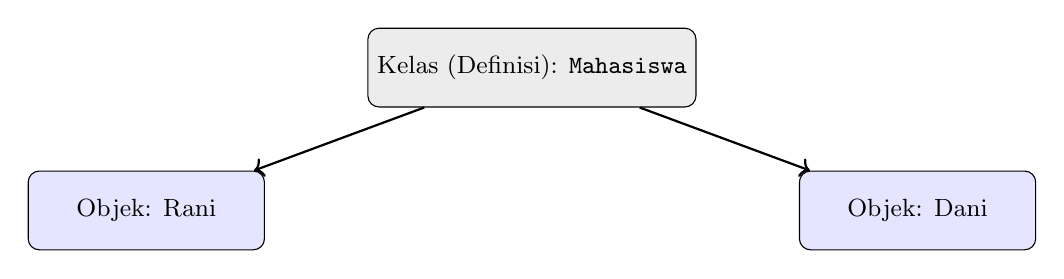
\begin{tikzpicture}[node distance=2.8cm, every node/.style={font=\small}]
\node (class) [draw, rectangle, rounded corners, fill=gray!15, minimum width=4cm, minimum height=1cm] {Kelas (Definisi): \texttt{Mahasiswa}};
\node (obj1) [below left=0.8cm and 1.3cm of class, draw, rectangle, rounded corners, fill=blue!10, minimum width=3cm, minimum height=1cm] {Objek: Rani};
\node (obj2) [below right=0.8cm and 1.3cm of class, draw, rectangle, rounded corners, fill=blue!10, minimum width=3cm, minimum height=1cm] {Objek: Dani};
\draw[->, thick] (class) -- (obj1);
\draw[->, thick] (class) -- (obj2);
\end{tikzpicture}
\end{center}

\subsection*{Ringkasan}
\begin{itemize}
    \item Kelas adalah \textbf{cetak biru sekaligus definisi} yang mendeskripsikan apa itu objek.
    \item Objek adalah \textbf{wujud nyata} dari definisi tersebut di dalam program.
    \item Semua objek dari kelas yang sama mengikuti struktur dan perilaku yang sama, namun memiliki data sendiri-sendiri.
\end{itemize}


\section{Atribut dan Metode}

\textbf{Atribut} dan \textbf{metode} merupakan dua komponen utama dalam kelas.  
Atribut menyimpan \emph{data atau keadaan} dari objek, sedangkan metode mendefinisikan \emph{perilaku atau aksi} yang dapat dilakukan objek.

Dengan kata lain, atribut menggambarkan \emph{apa yang dimiliki} oleh objek, dan metode menggambarkan \emph{apa yang dapat dilakukan} oleh objek tersebut.

\subsection{Atribut Instans dan Kelas}

Atribut dalam Python terbagi menjadi dua jenis utama:
\begin{enumerate}
    \item \textbf{Atribut Instans} — dimiliki secara unik oleh setiap objek (disimpan di dalam \texttt{self}).
    \item \textbf{Atribut Kelas} — dimiliki bersama oleh semua objek dari kelas yang sama.
\end{enumerate}

\noindent\textbf{Contoh Atribut Instans:}
Atribut ini didefinisikan di dalam konstruktor \texttt{__init__()} dan berbeda untuk setiap objek.

\begin{lstlisting}[style=PythonStyle, caption={Atribut Instans}]
class Mahasiswa:
    def __init__(self, nama, nim):
        self.nama = nama      # atribut instans
        self.nim = nim        # atribut instans

m1 = Mahasiswa("Rani", "A11.2024.0001")
m2 = Mahasiswa("Dani", "A11.2024.0002")

print(m1.nama)  # Rani
print(m2.nama)  # Dani
\end{lstlisting}

Pada contoh di atas, \texttt{m1.nama} dan \texttt{m2.nama} adalah atribut instans yang menyimpan data berbeda pada setiap objek.

\noindent\textbf{Contoh Atribut Kelas:}
Atribut kelas dideklarasikan di luar konstruktor dan nilainya sama untuk semua objek.

\begin{lstlisting}[style=PythonStyle, caption={Atribut Kelas}]
class Mahasiswa:
    universitas = "Pradita University"  # atribut kelas

    def __init__(self, nama, nim):
        self.nama = nama
        self.nim = nim

m1 = Mahasiswa("Rani", "A11.2024.0001")
m2 = Mahasiswa("Dani", "A11.2024.0002")

print(m1.universitas)  # Pradita University
print(m2.universitas)  # Pradita University
\end{lstlisting}

Jika nilai atribut kelas diubah dari nama kelasnya, maka perubahan akan berlaku untuk semua objek.

\begin{lstlisting}[style=PythonStyle, caption={Perubahan Atribut Kelas}]
Mahasiswa.universitas = "Universitas Python"

print(m1.universitas)  # Universitas Python
print(m2.universitas)  # Universitas Python
\end{lstlisting}

\noindent\textbf{Perbedaan Penting:}
\begin{itemize}
    \item Atribut instans: menyimpan data spesifik tiap objek.
    \item Atribut kelas: digunakan bersama oleh semua objek dari kelas tersebut.
\end{itemize}

\subsection{Metode dan \texttt{self}}

Metode adalah fungsi yang didefinisikan di dalam kelas. Metode digunakan untuk mendeskripsikan \textbf{perilaku} dari objek.  
Setiap metode memiliki parameter pertama bernama \texttt{self}, yang mereferensikan objek yang memanggil metode tersebut.

\begin{lstlisting}[style=PythonStyle, caption={Metode dengan self}]
class Mahasiswa:
    def __init__(self, nama, nim):
        self.nama = nama
        self.nim = nim

    def sapa(self):
        print(f"Halo, saya {self.nama} ({self.nim})")

m1 = Mahasiswa("Rani", "A11.2024.0001")
m2 = Mahasiswa("Dani", "A11.2024.0002")

m1.sapa()
m2.sapa()
\end{lstlisting}

\noindent\textbf{Penjelasan:}
\begin{itemize}
    \item \texttt{self} selalu mengacu pada objek yang sedang aktif.
    \item Ketika kita memanggil \texttt{m1.sapa()}, Python secara otomatis meneruskan objek \texttt{m1} sebagai argumen pertama \texttt{self}.
    \item Dengan demikian, setiap metode dapat mengakses atribut milik objek yang memanggilnya.
\end{itemize}

\noindent\textbf{Contoh dengan Perilaku Tambahan:}
\begin{lstlisting}[style=PythonStyle, caption={Metode yang Mengubah Keadaan Objek}]
class Mobil:
    def __init__(self, merek, kecepatan=0):
        self.merek = merek
        self.kecepatan = kecepatan

    def tambah_kecepatan(self, delta):
        self.kecepatan += delta

    def info(self):
        print(f"{self.merek} melaju {self.kecepatan} km/jam")

mobil1 = Mobil("Toyota")
mobil1.tambah_kecepatan(50)
mobil1.info()
\end{lstlisting}

Dalam contoh di atas:
\begin{itemize}
    \item \texttt{tambah_kecepatan()} adalah metode yang mengubah \textbf{keadaan objek}.
    \item \texttt{info()} adalah metode untuk menampilkan \textbf{informasi dari keadaan tersebut}.
\end{itemize}

\subsection*{Hubungan Atribut dan Metode}
Kombinasi atribut dan metode menjadikan setiap objek \emph{hidup} — ia memiliki keadaan (data) dan perilaku (aksi).  
Keduanya tidak terpisahkan karena definisi objek selalu mencakup keduanya:  
\emph{"Apa yang dimiliki" dan "apa yang dapat dilakukan".}

\begin{center}
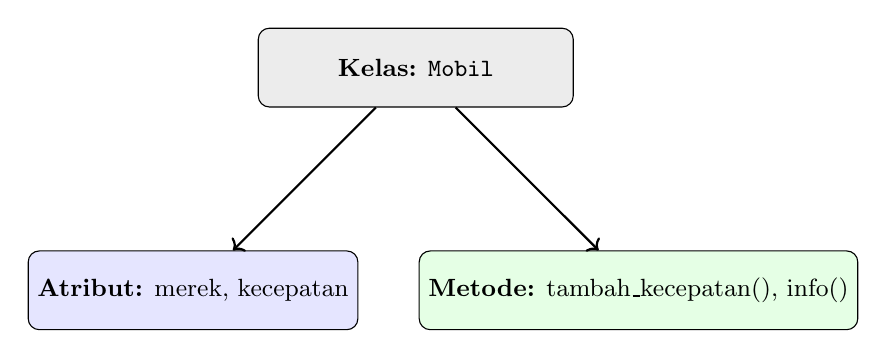
\begin{tikzpicture}[node distance=4cm, every node/.style={font=\small}]
\node (class) [draw, rectangle, rounded corners, fill=gray!15, minimum width=4cm, minimum height=1cm] {\textbf{Kelas:} \texttt{Mobil}};
\node (attr) [below left of=class, draw, rectangle, rounded corners, fill=blue!10, minimum width=3cm, minimum height=1cm] {\textbf{Atribut:} merek, kecepatan};
\node (method) [below right of=class, draw, rectangle, rounded corners, fill=green!10, minimum width=3cm, minimum height=1cm] {\textbf{Metode:} tambah\_kecepatan(), info()};
\draw[->, thick] (class) -- (attr);
\draw[->, thick] (class) -- (method);
\end{tikzpicture}
\end{center}


\subsection*{Ringkasan}
\begin{itemize}
    \item \textbf{Atribut} menyimpan data atau keadaan objek.
    \item \textbf{Metode} mendefinisikan perilaku objek.
    \item \texttt{self} digunakan untuk mengakses atribut dan metode milik objek itu sendiri.
    \item Atribut kelas dimiliki bersama, sedangkan atribut instans spesifik untuk tiap objek.
\end{itemize}

\section{Pewarisan (Inheritance)}

\textbf{Pewarisan (Inheritance)} adalah salah satu konsep inti dalam pemrograman berorientasi objek (OOP).  
Konsep ini memungkinkan sebuah kelas untuk \textbf{mewarisi atribut dan metode dari kelas lain}.  
Dengan pewarisan, kita dapat membuat kelas baru yang mewarisi perilaku dari kelas yang sudah ada tanpa menulis ulang semua kodenya.

\begin{center}
\textit{Tujuan pewarisan adalah untuk memanfaatkan kembali kode dan membangun hierarki kelas yang lebih logis.}
\end{center}

\subsection{Konsep Pewarisan}

Kelas yang diwarisi disebut \textbf{kelas induk (superclass atau parent class)},  
sedangkan kelas yang mewarisi disebut \textbf{kelas turunan (subclass atau child class)}.  
Kelas turunan dapat:
\begin{itemize}
    \item Menggunakan atribut dan metode dari kelas induk.
    \item Menambahkan atribut atau metode baru.
    \item Menimpa (override) metode yang sudah ada untuk perilaku khusus.
\end{itemize}

\noindent\textbf{Contoh Pewarisan Sederhana:}

\begin{lstlisting}[style=PythonStyle, caption={Contoh Pewarisan Dasar}]
# Kelas induk
class Kendaraan:
    def __init__(self, merek):
        self.merek = merek

    def info(self):
        print(f"Kendaraan merek {self.merek}")

# Kelas turunan
class Mobil(Kendaraan):
    def __init__(self, merek, jumlah_pintu):
        self.merek = merek
        self.jumlah_pintu = jumlah_pintu

    def info(self):
        print(f"Mobil {self.merek} dengan {self.jumlah_pintu} pintu")

# Membuat objek
k1 = Kendaraan("Yamaha")
m1 = Mobil("Toyota", 4)

k1.info()
m1.info()
\end{lstlisting}

Kelas \texttt{Mobil} di atas mewarisi struktur dari \texttt{Kendaraan}, tetapi menambahkan atribut baru (\texttt{jumlah\_pintu}) dan menimpa metode \texttt{info()} untuk menampilkan perilaku yang berbeda.

\begin{center}
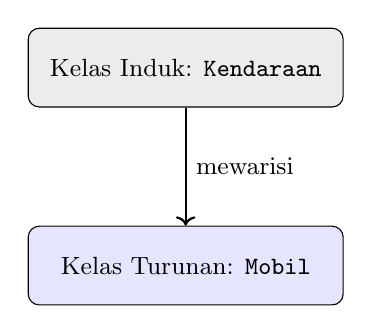
\begin{tikzpicture}[node distance=2.8cm, every node/.style={font=\small}]
\node (super) [draw, rectangle, rounded corners, fill=gray!15, minimum width=4cm, minimum height=1cm] {Kelas Induk: \texttt{Kendaraan}};
\node (child) [below=1.5cm of super, draw, rectangle, rounded corners, fill=blue!10, minimum width=4cm, minimum height=1cm] {Kelas Turunan: \texttt{Mobil}};
\draw[->, thick] (super) -- (child) node[midway, right] {mewarisi};
\end{tikzpicture}
\end{center}

\noindent\textbf{Manfaat Pewarisan:}
\begin{itemize}
    \item Menghindari duplikasi kode.
    \item Memudahkan perluasan (ekstensi) fungsi program.
    \item Menyusun hubungan hierarkis yang alami antar kelas.
\end{itemize}

\noindent\textbf{Contoh Hierarki Pewarisan Lebih Dalam:}

\begin{lstlisting}[style=PythonStyle, caption={Hierarki Tiga Tingkat}]
class Kendaraan:
    def bergerak(self):
        print("Kendaraan bergerak")

class Mobil(Kendaraan):
    def bergerak(self):
        print("Mobil melaju di jalan")

class MobilBalap(Mobil):
    def bergerak(self):
        print("Mobil balap melaju sangat cepat!")

# Objek dari masing-masing kelas
k = Kendaraan()
m = Mobil()
mb = MobilBalap()

for obj in [k, m, mb]:
    obj.bergerak()
\end{lstlisting}

Kode di atas memperlihatkan konsep pewarisan bertingkat (multi-level inheritance).  
Setiap kelas dapat menimpa metode \texttt{bergerak()} dengan perilaku yang semakin spesifik.

\subsection{Menggunakan \texttt{super()}}

Ketika kelas turunan memiliki konstruktor sendiri, kita sering kali masih ingin memanggil konstruktor dari kelas induk agar atribut dasarnya juga diinisialisasi.  
Untuk itu, Python menyediakan fungsi \texttt{super()}.

\noindent\textbf{Contoh Penggunaan \texttt{super()}:}

\begin{lstlisting}[style=PythonStyle, caption={Menggunakan super() untuk Memanggil Konstruktor Induk}]
class Kendaraan:
    def __init__(self, merek):
        self.merek = merek

class Mobil(Kendaraan):
    def __init__(self, merek, jumlah_pintu):
        super().__init__(merek)   # memanggil konstruktor kelas induk
        self.jumlah_pintu = jumlah_pintu

    def info(self):
        print(f"{self.merek} - {self.jumlah_pintu} pintu")

m1 = Mobil("Honda", 4)
m1.info()
\end{lstlisting}

Tanpa \texttt{super()}, kita harus menulis ulang inisialisasi atribut dari kelas induk, yang berpotensi menyebabkan duplikasi kode.

\textbf{Catatan Penting tentang \texttt{super()}:}
\begin{itemize}
    \item \texttt{super()} digunakan untuk mengakses metode atau konstruktor dari kelas induk.
    \item Umumnya dipakai di dalam metode \texttt{__init__()} agar atribut induk tetap terinisialisasi.
    \item Mendukung pewarisan bertingkat — Python secara otomatis mengikuti urutan hierarki kelas (\textbf{Method Resolution Order, MRO}).
\end{itemize}

\noindent\textbf{Contoh Pewarisan Bertingkat dengan \texttt{super()}:}

\begin{lstlisting}[style=PythonStyle, caption={super() dalam Pewarisan Bertingkat}]
class Kendaraan:
    def __init__(self):
        print("Kendaraan dibuat")

class Mobil(Kendaraan):
    def __init__(self):
        super().__init__()
        print("Mobil dibuat")

class MobilBalap(Mobil):
    def __init__(self):
        super().__init__()
        print("Mobil balap dibuat")

obj = MobilBalap()
\end{lstlisting}

Output:
\begin{lstlisting}[language=bash, caption={Output Program}]
Kendaraan dibuat
Mobil dibuat
Mobil balap dibuat
\end{lstlisting}

\subsection*{Ringkasan}
\begin{itemize}
    \item Pewarisan memungkinkan kelas baru menggunakan ulang kode dari kelas lain.
    \item Kelas induk = sumber definisi, kelas turunan = perluasan atau penyesuaian.
    \item \texttt{super()} digunakan untuk memanggil metode dari kelas induk, biasanya dalam konstruktor.
    \item Pewarisan mendukung hierarki bertingkat dan konsep polimorfisme.
\end{itemize}


\section{Polimorfisme}

\textbf{Polimorfisme (Polymorphism)} berasal dari bahasa Yunani: \emph{poly} berarti banyak, dan \emph{morph} berarti bentuk.  
Dalam konteks OOP, polimorfisme berarti bahwa \textbf{satu antarmuka dapat digunakan untuk berbagai bentuk objek yang berbeda}.  
Setiap objek dapat merespons cara yang sama (\emph{method call}) dengan perilaku yang berbeda-beda.

\begin{center}
\textit{Dengan polimorfisme, objek-objek dari kelas turunan dapat digunakan seolah-olah mereka adalah objek dari kelas induk.}
\end{center}

Polimorfisme membuat kode lebih fleksibel, mudah diperluas, dan tidak perlu diubah setiap kali jenis objek baru ditambahkan.

\subsection{Konsep Polimorfisme dan Overriding}

Polimorfisme biasanya muncul bersama dengan \textbf{pewarisan} dan \textbf{overriding}.  
Overriding berarti kelas turunan menulis ulang (menimpa) metode dari kelas induk untuk memberikan perilaku yang berbeda sesuai konteksnya sendiri.

\textbf{Contoh Sederhana Polimorfisme:}

\begin{lstlisting}[style=PythonStyle, caption={Polimorfisme dengan Overriding}]
class Hewan:
    def suara(self):
        print("Hewan mengeluarkan suara.")

class Kucing(Hewan):
    def suara(self):
        print("Meong")

class Anjing(Hewan):
    def suara(self):
        print("Guk guk")

# Semua objek dapat diperlakukan sama (sebagai Hewan)
hewan_list = [Hewan(), Kucing(), Anjing()]

for h in hewan_list:
    h.suara()
\end{lstlisting}

\begin{lstlisting}[language=bash, caption={Output Program}]
Hewan mengeluarkan suara.
Meong
Guk guk
\end{lstlisting}

Dalam contoh di atas:
\begin{itemize}
    \item Semua kelas (\texttt{Hewan}, \texttt{Kucing}, \texttt{Anjing}) memiliki metode \texttt{suara()}.
    \item Implementasinya berbeda untuk setiap kelas.
    \item Ketika loop \texttt{for h in hewan\_list} dijalankan, Python secara otomatis memanggil versi metode yang sesuai dengan objeknya.
\end{itemize}

\textbf{Polimorfisme Tanpa Pewarisan Langsung (Duck Typing):}

Python mendukung konsep \textbf{duck typing} —  
yaitu bentuk polimorfisme di mana tipe objek tidak perlu sama, selama objek memiliki metode yang dibutuhkan.

\begin{lstlisting}[style=PythonStyle, caption={Contoh Duck Typing}]
class Burung:
    def terbang(self):
        print("Burung terbang di langit.")

class Pesawat:
    def terbang(self):
        print("Pesawat lepas landas di landasan.")

# Fungsi yang menerima objek apa pun yang punya metode terbang()
def uji_terbang(obj):
    obj.terbang()

uji_terbang(Burung())
uji_terbang(Pesawat())
\end{lstlisting}

\begin{lstlisting}[language=bash, caption={Output Program}]
Burung terbang di langit.
Pesawat lepas landas di landasan.
\end{lstlisting}

Konsep ini disebut “duck typing” dari pepatah:
\begin{center}
\textit{“If it walks like a duck and quacks like a duck, it’s probably a duck.”}
\end{center}

Artinya, Python tidak peduli dari kelas mana objek berasal —  
selama objek memiliki metode yang diharapkan, maka objek tersebut dapat digunakan.

\textbf{Polimorfisme dalam Hierarki Kelas:}

\begin{lstlisting}[style=PythonStyle, caption={Hierarki Pewarisan dengan Polimorfisme}]
class Kendaraan:
    def bergerak(self):
        print("Kendaraan bergerak.")

class Mobil(Kendaraan):
    def bergerak(self):
        print("Mobil melaju di jalan.")

class Kapal(Kendaraan):
    def bergerak(self):
        print("Kapal berlayar di laut.")

class Pesawat(Kendaraan):
    def bergerak(self):
        print("Pesawat terbang di udara.")

kendaraan_list = [Mobil(), Kapal(), Pesawat()]

for k in kendaraan_list:
    k.bergerak()
\end{lstlisting}

\begin{lstlisting}[language=bash, caption={Output Program}]
Mobil melaju di jalan.
Kapal berlayar di laut.
Pesawat terbang di udara.
\end{lstlisting}

Setiap objek dapat dipanggil dengan cara yang sama, yaitu \texttt{k.bergerak()},  
namun hasil yang ditampilkan berbeda tergantung jenis objeknya — inilah hakikat dari polimorfisme.

\begin{center}
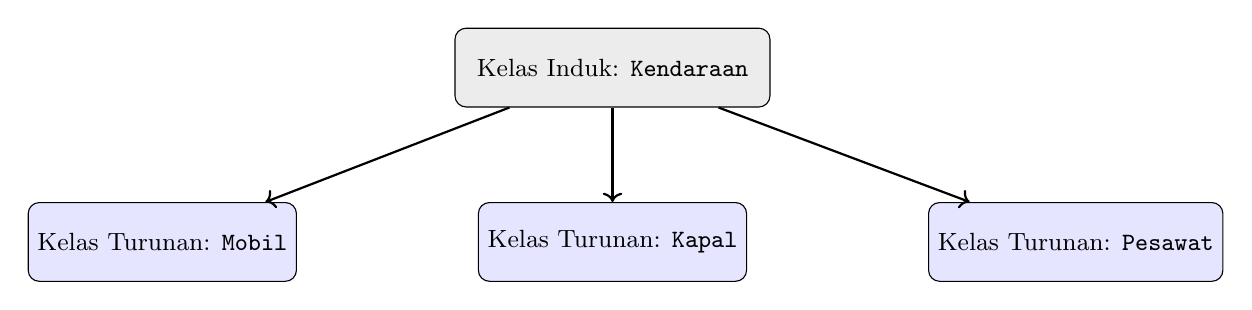
\begin{tikzpicture}[node distance=1.6cm, every node/.style={font=\small}]
\node (super) [draw, rectangle, rounded corners, fill=gray!15, minimum width=4cm, minimum height=1cm] {Kelas Induk: \texttt{Kendaraan}};
\node (mobil) [below left=1.2cm and 2.0cm of super, draw, rectangle, rounded corners, fill=blue!10, minimum width=3cm, minimum height=1cm] {Kelas Turunan: \texttt{Mobil}};
\node (kapal) [below=1.2cm of super, draw, rectangle, rounded corners, fill=blue!10, minimum width=3cm, minimum height=1cm] {Kelas Turunan: \texttt{Kapal}};
\node (pesawat) [below right=1.2cm and 2.0cm of super, draw, rectangle, rounded corners, fill=blue!10, minimum width=3cm, minimum height=1cm] {Kelas Turunan: \texttt{Pesawat}};
\draw[->, thick] (super) -- (mobil);
\draw[->, thick] (super) -- (kapal);
\draw[->, thick] (super) -- (pesawat);
\end{tikzpicture}
\end{center}

\subsection*{Ringkasan}
\begin{itemize}
    \item Polimorfisme memungkinkan satu metode dipanggil pada berbagai objek dengan hasil yang berbeda.
    \item Overriding terjadi ketika kelas turunan menimpa metode kelas induk.
    \item Python mendukung polimorfisme baik melalui pewarisan maupun \emph{duck typing}.
    \item Dengan polimorfisme, kode menjadi lebih fleksibel, mudah diperluas, dan alami dalam menggambarkan perilaku dunia nyata.
\end{itemize}

\section{Latihan}

Bagian ini berisi latihan praktis untuk memperdalam pemahaman konsep OOP di Python — mencakup kelas, objek, atribut, metode, pewarisan, dan polimorfisme.  
Setiap latihan dirancang agar mahasiswa dapat mempraktikkan konsep secara bertahap, mulai dari dasar hingga penerapan dalam konteks nyata.

\subsection*{Latihan 1: Membuat Kelas dan Objek}
Buat sebuah kelas bernama \texttt{Mahasiswa} dengan ketentuan berikut:
\begin{enumerate}
    \item Memiliki atribut \texttt{nama}, \texttt{nim}, dan \texttt{jurusan}.
    \item Memiliki metode \texttt{tampilkan\_info()} yang menampilkan semua atribut di layar.
    \item Buat minimal dua objek dari kelas tersebut dan panggil metode \texttt{tampilkan\_info()} untuk masing-masing.
\end{enumerate}

\begin{lstlisting}[style=PythonStyle, caption={Contoh keluaran yang diharapkan (tidak harus identik)}]
Nama: Rani
NIM: A11.2024.0001
Jurusan: Informatika

Nama: Dani
NIM: A11.2024.0002
Jurusan: Sistem Informasi
\end{lstlisting}

\subsection*{Latihan 2: Atribut dan Metode}
Kembangkan kelas \texttt{Mahasiswa} sebelumnya dengan:
\begin{enumerate}
    \item Menambahkan atribut kelas bernama \texttt{universitas}.
    \item Membuat metode baru \texttt{ubah\_jurusan(jurusan\_baru)} yang mengubah nilai atribut \texttt{jurusan}.
    \item Panggil metode tersebut dan tampilkan hasil perubahan.
\end{enumerate}

\subsection*{Latihan 3: Pewarisan}
Buat hierarki kelas berikut:
\begin{itemize}
    \item Kelas induk: \texttt{Kendaraan} dengan atribut \texttt{merek} dan metode \texttt{bergerak()}.
    \item Kelas turunan: \texttt{Mobil} dan \texttt{SepedaMotor}, masing-masing menimpa metode \texttt{bergerak()}.
    \item Tambahkan konstruktor di setiap kelas dan panggil konstruktor induk menggunakan \texttt{super()}.
\end{itemize}

\begin{lstlisting}[style=PythonStyle, caption={Contoh penggunaan}]
k1 = Mobil("Toyota")
k2 = SepedaMotor("Honda")

k1.bergerak()
k2.bergerak()
\end{lstlisting}

\begin{lstlisting}[language=bash, caption={Output Program}]
Mobil Toyota melaju di jalan raya.
Sepeda motor Honda berjalan di aspal.
\end{lstlisting}

\subsection*{Latihan 4: Polimorfisme}
Buat fungsi \texttt{uji\_bergerak(kendaraan)} yang menerima objek apa pun yang memiliki metode \texttt{bergerak()}.  
Gunakan kelas-kelas dari latihan sebelumnya (\texttt{Kendaraan}, \texttt{Mobil}, \texttt{SepedaMotor}), dan tambahkan satu kelas baru \texttt{Pesawat} yang juga memiliki metode \texttt{bergerak()}.

\begin{enumerate}
    \item Buat daftar berisi beberapa objek dari kelas berbeda.
    \item Gunakan satu loop untuk memanggil \texttt{bergerak()} pada semuanya.
\end{enumerate}

\begin{lstlisting}[language=bash, caption={Output yang Diharapkan}]
Mobil Toyota melaju di jalan raya.
Sepeda motor Honda berjalan di aspal.
Pesawat Garuda terbang di udara.
\end{lstlisting}

\subsection*{Latihan 5: Studi Kasus Mini — Sistem Geometri Bangun Datar}

Rancang sebuah program kecil untuk mendemonstrasikan seluruh konsep OOP yang telah dipelajari melalui perhitungan luas berbagai bangun datar.

\textbf{Deskripsi:}
\begin{itemize}
    \item Buat kelas induk \texttt{BangunDatar} dengan metode \texttt{luas()}.
    \item Buat kelas turunan \texttt{Persegi}, \texttt{PersegiPanjang}, dan \texttt{Lingkaran} yang menimpa metode \texttt{luas()}.
    \item Tambahkan atribut yang sesuai untuk tiap bangun (misalnya \texttt{sisi}, \texttt{panjang}, \texttt{lebar}, \texttt{jari\_jari}).
    \item Gunakan polimorfisme untuk menghitung luas semua bangun dalam satu loop.
\end{itemize}

\begin{lstlisting}[style=PythonStyle, caption={Contoh Implementasi}]
import math

class BangunDatar:
    def luas(self):
        print("Metode luas() harus dioverride di kelas turunan")

class Persegi(BangunDatar):
    def __init__(self, sisi):
        self.sisi = sisi
    def luas(self):
        return self.sisi * self.sisi

class PersegiPanjang(BangunDatar):
    def __init__(self, panjang, lebar):
        self.panjang = panjang
        self.lebar = lebar
    def luas(self):
        return self.panjang * self.lebar

class Lingkaran(BangunDatar):
    def __init__(self, jari_jari):
        self.jari_jari = jari_jari
    def luas(self):
        return math.pi * self.jari_jari ** 2

# Daftar objek dari berbagai kelas turunan
bangun_list = [
    Persegi(5),
    PersegiPanjang(4, 6),
    Lingkaran(7)
]

# Menghitung luas setiap bangun secara polimorfik
for b in bangun_list:
    print(f"Luas {b.__class__.__name__}: {b.luas():.2f}")
\end{lstlisting}

\begin{lstlisting}[language=bash, caption={Output Program}]
Luas Persegi: 25.00
Luas PersegiPanjang: 24.00
Luas Lingkaran: 153.94
\end{lstlisting}

\textbf{Tujuan:}
\begin{itemize}
    \item Menunjukkan bahwa setiap kelas turunan dapat memiliki perilaku (metode) yang berbeda, meskipun memiliki antarmuka yang sama.
    \item Mempraktikkan penggunaan pewarisan dan overriding dalam konteks yang realistis.
    \item Memahami bagaimana polimorfisme memudahkan pemrosesan banyak objek dalam satu struktur kode yang seragam.
\end{itemize}


\subsection*{Refleksi dan Diskusi}
Setelah menyelesaikan seluruh latihan, jawab pertanyaan berikut:
\begin{enumerate}
    \item Apa perbedaan utama antara atribut kelas dan atribut instans?
    \item Mengapa penggunaan \texttt{super()} penting dalam pewarisan?
    \item Bagaimana polimorfisme membantu membuat kode lebih fleksibel?
    \item Apa manfaat praktis konsep OOP dalam membangun aplikasi dunia nyata?
\end{enumerate}

\section{Ringkasan}
	
Bab ini membahas konsep dasar pemrograman berorientasi objek (OOP) di Python, meliputi kelas, objek, atribut, metode, pewarisan, dan polimorfisme. Setiap bagian menekankan bagaimana kelas berfungsi sebagai cetak biru sekaligus definisi dari objek, bagaimana atribut menyimpan keadaan, serta bagaimana metode mendefinisikan perilaku. Melalui konsep pewarisan dan penggunaan \texttt{super()}, mahasiswa dapat membuat hierarki kelas yang efisien dan menghindari duplikasi kode.

Selain itu, bab ini memperkenalkan polimorfisme sebagai kemampuan berbagai objek untuk merespons perintah yang sama dengan cara yang berbeda. Polimorfisme dan duck typing memberikan fleksibilitas tinggi dalam desain program, memungkinkan pengembang membuat sistem yang mudah diperluas, alami, dan sesuai dengan model dunia nyata. Pemahaman konsep-konsep ini menjadi fondasi penting untuk membangun program Python yang modular, dapat digunakan kembali, dan mudah dirawat.


	\chapter{Penanganan Kesalahan}

\section{Pendahuluan}

Dalam proses pemrograman, kesalahan atau error merupakan hal yang tidak dapat dihindari. Seorang pemrogram pemula sering kali menemukan programnya berhenti tiba-tiba, menampilkan pesan kesalahan yang panjang dan membingungkan. Namun, seiring dengan meningkatnya pemahaman, kesalahan tersebut dapat dilihat bukan sebagai kegagalan, melainkan sebagai bagian penting dari proses belajar dan pengembangan perangkat lunak.

Pada dasarnya, terdapat dua jenis kesalahan utama dalam Python: \textbf{kesalahan sintaks (syntax error)} dan \textbf{kesalahan saat berjalan (runtime error)}. Kesalahan sintaks terjadi ketika penulisan kode tidak sesuai dengan aturan bahasa Python, seperti tanda kurung yang tidak seimbang atau penggunaan kata kunci yang salah—jenis kesalahan ini terdeteksi sebelum program dijalankan. Sementara itu, kesalahan saat berjalan muncul ketika program telah dieksekusi dan terjadi kondisi yang tidak diharapkan, misalnya pembagian dengan nol atau akses indeks di luar jangkauan pada sebuah \textit{list}. Kesalahan saat berjalan inilah yang, di Python, dimodelkan sebagai \textbf{exception}.

Untuk menghadapi kondisi tak terduga tersebut, Python menyediakan mekanisme \textbf{exception handling} yang memungkinkan program mengantisipasi dan menangani kesalahan tanpa harus berhenti secara mendadak. Alih-alih gagal total, program dapat menampilkan pesan yang lebih ramah, melakukan langkah pemulihan (\textit{recovery}), atau melakukan pembersihan sumber daya dengan rapi. Pada bab ini, Anda akan mempelajari cara kerja blok \texttt{try-except}, bagaimana menulis penanganan untuk \textit{banyak} jenis exception, penggunaan \texttt{else} (dijalankan ketika tidak ada error) dan \texttt{finally} (selalu dijalankan untuk \textit{cleanup}), serta cara membuat \textbf{custom exception} untuk mengekspresikan aturan domain secara lebih jelas. Tujuannya adalah agar Anda mampu menulis program Python yang \textit{robust}, informatif saat terjadi error, dan mudah dirawat.


\section{Konsep Dasar Exception}

Dalam pemrograman, kesalahan atau \textit{error} merupakan kondisi yang menyebabkan program tidak dapat berjalan sebagaimana mestinya. Python memiliki cara sistematis untuk menangani kesalahan ini agar program tetap dapat berfungsi dengan baik. Sebelum memahami bagaimana cara menanganinya, penting untuk mengetahui jenis-jenis kesalahan yang mungkin terjadi serta konsep dasar yang mendasari \textbf{exception}.

\subsection*{Kesalahan Sintaks (Syntax Error)}

Kesalahan sintaks terjadi ketika penulisan kode tidak sesuai dengan aturan bahasa Python. Interpreter Python akan mendeteksi kesalahan ini sebelum program dijalankan. Karena itu, kesalahan sintaks mencegah program untuk dieksekusi sama sekali.

\begin{lstlisting}[style=PythonStyle, caption={Contoh kesalahan sintaks}]
# Contoh kesalahan sintaks: tanda kurung kurang
print("Halo dunia"
\end{lstlisting}

Ketika dijalankan, Python akan menampilkan pesan kesalahan seperti berikut:

\begin{lstlisting}[language=bash]
SyntaxError: unexpected EOF while parsing
\end{lstlisting}

Pesan tersebut menandakan bahwa interpreter mendeteksi akhir baris yang tidak sesuai harapan — dalam hal ini, karena tanda kurung penutup tidak ada.

\subsection*{Kesalahan Saat Berjalan (Runtime Error)}

Kesalahan jenis ini hanya muncul ketika program dijalankan. Artinya, kode sudah benar secara sintaks, tetapi ketika dijalankan muncul kondisi yang tidak dapat ditangani. Contoh paling umum adalah pembagian dengan nol.

\begin{lstlisting}[style=PythonStyle, caption={Contoh kesalahan runtime}]
# Contoh kesalahan runtime: pembagian dengan nol
hasil = 10 / 0
print(hasil)
\end{lstlisting}

Ketika dijalankan, Python akan menampilkan pesan seperti berikut:

\begin{lstlisting}[language=bash]
ZeroDivisionError: division by zero
\end{lstlisting}

Berbeda dengan kesalahan sintaks, kesalahan runtime tidak menghentikan keseluruhan program secara permanen — kita dapat menangkapnya dengan mekanisme khusus agar program tetap berjalan. Kesalahan seperti inilah yang disebut \textbf{exception}.

\subsection*{Apa Itu Exception?}

\textbf{Exception} adalah peristiwa (event) yang terjadi selama eksekusi program dan mengganggu alur normal instruksi. Python memiliki berbagai jenis exception bawaan seperti:

\begin{itemize}
    \item \texttt{ZeroDivisionError} – pembagian dengan nol,
    \item \texttt{IndexError} – akses indeks list di luar jangkauan,
    \item \texttt{ValueError} – kesalahan pada nilai atau tipe data,
    \item \texttt{FileNotFoundError} – file yang diminta tidak ditemukan,
    \item \texttt{TypeError} – operasi dilakukan pada tipe data yang tidak sesuai.
\end{itemize}

Contoh berikut memperlihatkan beberapa exception umum:

\begin{lstlisting}[style=PythonStyle, caption={Beberapa contoh exception umum}]
# IndexError
angka = [1, 2, 3]
print(angka[5])

# ValueError
int("abc")

# FileNotFoundError
with open("data.txt") as f:
    isi = f.read()
\end{lstlisting}

Setiap contoh di atas akan menghasilkan jenis exception yang berbeda.

\subsection*{Mengapa Perlu Menangani Exception?}

Tanpa mekanisme penanganan exception, setiap kesalahan yang terjadi akan langsung menghentikan program. Dalam aplikasi nyata, hal ini tidak dapat diterima, terutama ketika program berinteraksi dengan pengguna atau sistem eksternal seperti file, jaringan, atau basis data. Misalnya, jika pengguna salah mengetikkan nama file, seharusnya program tidak langsung berhenti, melainkan menampilkan pesan yang ramah seperti:

\begin{lstlisting}[language=bash]
File tidak ditemukan. Silakan periksa kembali nama file Anda.
\end{lstlisting}

Penanganan exception membantu:
\begin{enumerate}
    \item Mencegah program berhenti secara tiba-tiba.
    \item Memberikan pesan kesalahan yang lebih informatif bagi pengguna.
    \item Menjaga keandalan (\textit{robustness}) dan kestabilan program.
    \item Memudahkan proses debugging dan pengujian.
\end{enumerate}

Dengan kata lain, penanganan exception adalah langkah penting menuju program yang profesional dan tangguh. Pada bagian berikutnya, kita akan mempelajari bagaimana Python menyediakan struktur \texttt{try-except} untuk menangani exception secara sistematis.


\section{Blok Try-Except}

Setelah memahami konsep dasar exception, langkah selanjutnya adalah mempelajari bagaimana Python menangani kesalahan tersebut tanpa membuat program berhenti. Untuk itu, Python menyediakan mekanisme yang disebut dengan \textbf{blok \texttt{try-except}}.

\subsection*{Struktur Dasar Try-Except}

Blok \texttt{try-except} digunakan untuk mencoba menjalankan potongan kode yang mungkin menghasilkan error, dan menangkap kesalahan tersebut jika benar terjadi. Dengan demikian, alur program tetap dapat dilanjutkan secara normal.

Struktur umumnya dapat ditulis sebagai berikut:

\begin{lstlisting}[style=PythonStyle, caption={Struktur dasar try-except di Python}]
try:
    # Kode yang mungkin menimbulkan exception
    operasi_berisiko()
except JenisException:
    # Kode yang dijalankan jika exception terjadi
    tangani_exception()
\end{lstlisting}

Alur eksekusinya sederhana:
\begin{enumerate}
    \item Python akan mengeksekusi blok \texttt{try}.
    \item Jika tidak ada kesalahan, blok \texttt{except} akan dilewati.
    \item Jika terjadi kesalahan, Python akan mencari blok \texttt{except} yang sesuai dan menjalankannya.
\end{enumerate}

Dengan cara ini, program tidak langsung berhenti saat error muncul — melainkan “menangkap” kesalahan dan bereaksi dengan cara yang lebih terkendali.

\subsection*{Contoh Sederhana Penanganan Exception}

Perhatikan contoh berikut. Kita mencoba membagi dua angka yang diinput oleh pengguna, tetapi bisa saja pengguna memasukkan nilai nol yang menyebabkan error pembagian.

\begin{lstlisting}[style=PythonStyle, caption={Contoh sederhana penggunaan try-except}]
try:
    a = int(input("Masukkan angka pertama: "))
    b = int(input("Masukkan angka kedua: "))
    hasil = a / b
    print("Hasil pembagian:", hasil)
except ZeroDivisionError:
    print("Error: Tidak dapat membagi dengan nol!")
\end{lstlisting}

Jika pengguna memasukkan nilai kedua sebagai nol, maka keluaran program akan seperti berikut:

\begin{lstlisting}[language=bash]
Masukkan angka pertama: 10
Masukkan angka kedua: 0
Error: Tidak dapat membagi dengan nol!
\end{lstlisting}

Sedangkan jika pengguna memasukkan dua angka valid, program akan menampilkan hasil pembagiannya tanpa gangguan.

\begin{lstlisting}[language=bash]
Masukkan angka pertama: 10
Masukkan angka kedua: 2
Hasil pembagian: 5.0
\end{lstlisting}

Dengan demikian, meskipun terjadi kesalahan, program tidak berhenti secara tiba-tiba — melainkan menampilkan pesan kesalahan yang lebih mudah dipahami pengguna.

\subsection*{Menangkap Semua Jenis Kesalahan}

Kadang kita tidak tahu secara pasti jenis kesalahan apa yang akan terjadi. Dalam kasus seperti itu, kita dapat menangkap semua jenis exception tanpa menyebutkan nama exception-nya.

\begin{lstlisting}[style=PythonStyle, caption={Menangkap semua jenis exception}]
try:
    x = int(input("Masukkan angka: "))
    y = 10 / x
    print("Hasil:", y)
except:
    print("Terjadi kesalahan yang tidak diketahui.")
\end{lstlisting}

Namun, praktik ini \textbf{tidak disarankan} untuk program besar, karena menyulitkan proses debugging — kita tidak tahu jenis kesalahan apa yang sebenarnya terjadi. Sebaiknya selalu tangani exception yang spesifik bila memungkinkan.

\subsection*{Menggunakan Pesan Error Kustom}

Selain menampilkan pesan umum, kita dapat menampilkan pesan yang lebih informatif dengan menangkap objek exception. Python memungkinkan kita mendapatkan detail error melalui kata kunci \texttt{as}.

\begin{lstlisting}[style=PythonStyle, caption={Penggunaan pesan error kustom}]
try:
    nama_file = input("Masukkan nama file: ")
    with open(nama_file) as f:
        isi = f.read()
        print("Isi file:", isi)
except FileNotFoundError as e:
    print("Terjadi kesalahan:", e)
    print("File tidak ditemukan. Silakan periksa nama file Anda.")
\end{lstlisting}

Contoh hasil eksekusi ketika pengguna memasukkan nama file yang salah:

\begin{lstlisting}[language=bash]
Masukkan nama file: data_tidak_ada.txt
Terjadi kesalahan: [Errno 2] No such file or directory: 'data_tidak_ada.txt'
File tidak ditemukan. Silakan periksa nama file Anda.
\end{lstlisting}

Dengan menampilkan pesan bawaan dari Python sekaligus menambahkan penjelasan sendiri, kita dapat membantu pengguna memahami sumber masalah sekaligus memberi arahan yang jelas.

\subsection*{Kesimpulan}

Blok \texttt{try-except} merupakan pondasi utama dalam penanganan kesalahan di Python. Ia memungkinkan program untuk:
\begin{itemize}
    \item Tetap berjalan meskipun terjadi error,
    \item Menyediakan pesan kesalahan yang ramah dan informatif,
    \item Mengontrol perilaku program saat situasi tak terduga muncul.
\end{itemize}

Pada bagian selanjutnya, kita akan memperluas konsep ini dengan menangani \textbf{beberapa jenis exception sekaligus} serta mempelajari bagaimana menambahkan blok tambahan seperti \texttt{else} dan \texttt{finally} untuk pengendalian alur yang lebih fleksibel.


\section{Menangani Beberapa Jenis Exception}

Dalam praktiknya, satu potongan kode bisa saja berpotensi menimbulkan berbagai jenis kesalahan. Misalnya, kesalahan input pengguna, pembagian dengan nol, atau file yang tidak ditemukan. Untuk menghadapi kondisi tersebut, Python memungkinkan kita menulis beberapa blok \texttt{except} agar setiap jenis exception dapat ditangani secara berbeda sesuai konteksnya.

\subsection*{Menangani Beberapa Exception Secara Terpisah}

Kita dapat menambahkan lebih dari satu blok \texttt{except} untuk menangani jenis kesalahan yang berbeda-beda. Dengan cara ini, program dapat memberikan respon yang lebih tepat sesuai dengan situasi yang terjadi.

\begin{lstlisting}[style=PythonStyle, caption={Menangani beberapa exception secara terpisah}]
try:
    a = int(input("Masukkan angka pertama: "))
    b = int(input("Masukkan angka kedua: "))
    hasil = a / b
    print("Hasil pembagian:", hasil)
except ZeroDivisionError:
    print("Error: Tidak dapat membagi dengan nol.")
except ValueError:
    print("Error: Input harus berupa angka, bukan teks.")
\end{lstlisting}

Berikut contoh hasil eksekusinya:

\begin{lstlisting}[language=bash]
Masukkan angka pertama: 10
Masukkan angka kedua: 0
Error: Tidak dapat membagi dengan nol.
\end{lstlisting}

\begin{lstlisting}[language=bash]
Masukkan angka pertama: sepuluh
Masukkan angka kedua: 2
Error: Input harus berupa angka, bukan teks.
\end{lstlisting}

Dengan pendekatan ini, setiap error yang berbeda dapat ditangani dengan cara yang lebih spesifik, sehingga pengguna mendapatkan informasi yang lebih akurat.

\subsection*{Menggabungkan Beberapa Exception dalam Satu Blok}

Terkadang beberapa jenis exception dapat ditangani dengan cara yang sama. Untuk kasus seperti ini, Python memungkinkan kita menulis beberapa nama exception dalam satu blok \texttt{except} menggunakan tanda kurung.

\begin{lstlisting}[style=PythonStyle, caption={Menggabungkan beberapa exception dalam satu blok}]
try:
    nilai = int(input("Masukkan angka: "))
    hasil = 100 / nilai
    print("Hasil:", hasil)
except (ZeroDivisionError, ValueError):
    print("Error: Input tidak valid atau pembagian dengan nol.")
\end{lstlisting}

Hasilnya akan sama baik ketika pengguna memasukkan nilai nol maupun teks yang tidak bisa diubah menjadi angka:

\begin{lstlisting}[language=bash]
Masukkan angka: 0
Error: Input tidak valid atau pembagian dengan nol.
\end{lstlisting}

\begin{lstlisting}[language=bash]
Masukkan angka: abc
Error: Input tidak valid atau pembagian dengan nol.
\end{lstlisting}

Teknik ini berguna ketika penanganan kedua jenis kesalahan cukup serupa dan tidak perlu dibedakan secara eksplisit.

\subsection*{Hierarki Exception di Python}

Python memiliki sistem hierarki exception di mana semua jenis kesalahan diturunkan dari kelas dasar \texttt{BaseException}. Sebagian besar exception yang sering kita tangani berasal dari turunan \texttt{Exception}.  
Gambaran sederhananya sebagai berikut:

\begin{center}
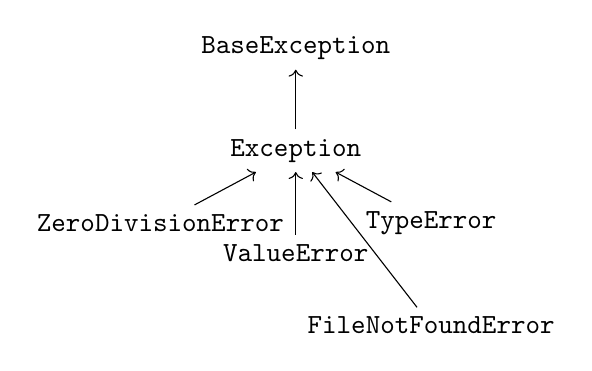
\begin{tikzpicture}[node distance=1.3cm, every node/.style={font=\ttfamily}]
\node (base) {BaseException};
\node (exc) [below of=base] {Exception};
\node (zero) [below left of=exc, xshift=-0.8cm] {ZeroDivisionError};
\node (value) [below of=exc] {ValueError};
\node (type) [below right of=exc, xshift=0.8cm] {TypeError};
\node (file) [below right of=value, xshift=0.8cm] {FileNotFoundError};
\draw[->] (exc) -- (base);
\draw[->] (zero) -- (exc);
\draw[->] (value) -- (exc);
\draw[->] (type) -- (exc);
\draw[->] (file) -- (exc);
\end{tikzpicture}
\end{center}

Artinya, jika kita menangkap \texttt{Exception} saja, maka semua jenis kesalahan yang merupakan turunannya juga akan tertangkap. Namun, untuk alasan kejelasan dan debugging yang efektif, sebaiknya kita menangkap jenis exception yang spesifik.

\begin{lstlisting}[style=PythonStyle, caption={Menangkap seluruh exception menggunakan kelas induk}]
try:
    x = int("abc")  # menyebabkan ValueError
except Exception as e:
    print("Terjadi kesalahan:", e)
\end{lstlisting}

Keluaran program:

\begin{lstlisting}[language=bash]
Terjadi kesalahan: invalid literal for int() with base 10: 'abc'
\end{lstlisting}

Dengan menangkap kelas induk \texttt{Exception}, semua jenis kesalahan turunan akan tertangani, tetapi kita tetap dapat mengakses detail error melalui variabel \texttt{e}.

\subsection*{Menggunakan \texttt{as} untuk Mendapatkan Objek Exception}

Dalam contoh sebelumnya, kita telah melihat bahwa kata kunci \texttt{as} digunakan untuk menangkap objek exception dan menyimpannya dalam variabel. Objek ini berisi informasi penting seperti pesan error, nama exception, dan atribut tambahan lainnya.

\begin{lstlisting}[style=PythonStyle, caption={Menggunakan 'as' untuk menangkap objek exception}]
try:
    angka = int(input("Masukkan angka: "))
    hasil = 100 / angka
    print("Hasil:", hasil)
except Exception as e:
    print("Tipe kesalahan:", type(e).__name__)
    print("Pesan kesalahan:", e)
\end{lstlisting}

Contoh hasil ketika pengguna memasukkan nilai nol:

\begin{lstlisting}[language=bash]
Masukkan angka: 0
Tipe kesalahan: ZeroDivisionError
Pesan kesalahan: division by zero
\end{lstlisting}

Atau jika pengguna memasukkan teks:

\begin{lstlisting}[language=bash]
Masukkan angka: abc
Tipe kesalahan: ValueError
Pesan kesalahan: invalid literal for int() with base 10: 'abc'
\end{lstlisting}

Dengan teknik ini, kita dapat menampilkan pesan yang lebih dinamis, mencatat error ke log, atau mengambil keputusan program secara otomatis berdasarkan jenis kesalahan yang terjadi.

\subsection*{Kesimpulan}

Pada bagian ini, kita telah mempelajari cara menangani lebih dari satu jenis exception, memahami hierarki exception di Python, dan menggunakan objek exception untuk memperoleh informasi lebih lanjut.  
Pendekatan ini membuat kode lebih \textit{robust}, mudah dirawat, serta lebih ramah bagi pengguna.  

Selanjutnya, kita akan membahas dua blok tambahan dalam penanganan exception, yaitu \texttt{else} dan \texttt{finally}, yang memberikan fleksibilitas lebih dalam mengontrol alur program.


\section{Blok Else dan Finally}

Selain blok \texttt{try} dan \texttt{except}, Python juga menyediakan dua blok tambahan yang dapat digunakan untuk mengontrol alur program secara lebih fleksibel, yaitu \texttt{else} dan \texttt{finally}. Kedua blok ini tidak wajib digunakan, tetapi sangat berguna untuk situasi tertentu, terutama ketika kita ingin memisahkan logika normal dari logika penanganan kesalahan, atau ketika kita perlu memastikan bahwa suatu tindakan pembersihan (\textit{cleanup}) tetap dilakukan meskipun terjadi error.

\subsection*{Blok Else}

Blok \texttt{else} digunakan setelah \texttt{except}, dan hanya akan dijalankan jika tidak terjadi exception dalam blok \texttt{try}. Dengan kata lain, kode di dalam \texttt{else} hanya berjalan ketika semua operasi di \texttt{try} berhasil.

Struktur lengkapnya sebagai berikut:

\begin{lstlisting}[style=PythonStyle, caption={Struktur lengkap try-except-else}]
try:
    # kode utama yang mungkin menyebabkan exception
except JenisException:
    # penanganan error
else:
    # kode ini hanya berjalan jika tidak ada error
\end{lstlisting}

Contoh penerapan:

\begin{lstlisting}[style=PythonStyle, caption={Penggunaan blok else}]
try:
    angka = int(input("Masukkan angka: "))
    hasil = 100 / angka
except ZeroDivisionError:
    print("Error: Pembagian dengan nol tidak diperbolehkan.")
except ValueError:
    print("Error: Input harus berupa angka.")
else:
    print("Hasil perhitungan:", hasil)
\end{lstlisting}

Hasil eksekusi ketika pengguna memasukkan angka valid:

\begin{lstlisting}[language=bash]
Masukkan angka: 5
Hasil perhitungan: 20.0
\end{lstlisting}

Dan ketika terjadi error:

\begin{lstlisting}[language=bash]
Masukkan angka: 0
Error: Pembagian dengan nol tidak diperbolehkan.
\end{lstlisting}

Blok \texttt{else} sangat bermanfaat untuk memisahkan logika utama dari logika penanganan error. Dengan begitu, struktur kode menjadi lebih bersih dan mudah dibaca.

\subsection*{Blok Finally}

Blok \texttt{finally} berfungsi untuk mengeksekusi kode yang harus dijalankan dalam kondisi apa pun — baik terjadi error maupun tidak. Biasanya, blok ini digunakan untuk melakukan tindakan pembersihan (\textit{cleanup}) seperti menutup file, melepaskan koneksi jaringan, atau menghapus data sementara.

\begin{lstlisting}[style=PythonStyle, caption={Struktur penggunaan blok finally}]
try:
    # operasi utama
except:
    # penanganan kesalahan
finally:
    # selalu dijalankan, baik ada error maupun tidak
\end{lstlisting}

Contoh penerapan nyata: membaca file dan memastikan file selalu ditutup.

\begin{lstlisting}[style=PythonStyle, caption={Contoh penggunaan finally untuk pembersihan}]
try:
    f = open("data.txt", "r")
    isi = f.read()
    print("Isi file:", isi)
except FileNotFoundError:
    print("Error: File tidak ditemukan.")
finally:
    print("Menutup file...")
    f.close()
\end{lstlisting}

Jika file tidak ditemukan, maka hasilnya:

\begin{lstlisting}[language=bash]
Error: File tidak ditemukan.
Menutup file...
Traceback (most recent call last):
  File "contoh.py", line 8, in <module>
    f.close()
UnboundLocalError: local variable 'f' referenced before assignment
\end{lstlisting}

Terjadi error baru karena variabel \texttt{f} belum pernah dibuat. Untuk menghindarinya, sebaiknya kita melakukan pemeriksaan terlebih dahulu sebelum menutup file.

\begin{lstlisting}[style=PythonStyle, caption={Menangani variabel dengan aman di finally}]
f = None
try:
    f = open("data.txt", "r")
    isi = f.read()
    print("Isi file:", isi)
except FileNotFoundError:
    print("Error: File tidak ditemukan.")
finally:
    if f is not None:
        f.close()
        print("File berhasil ditutup.")
\end{lstlisting}

Hasil keluaran saat file tidak ada:

\begin{lstlisting}[language=bash]
Error: File tidak ditemukan.
\end{lstlisting}

Dan ketika file ada:

\begin{lstlisting}[language=bash]
Isi file: Halo, ini contoh isi file.
File berhasil ditutup.
\end{lstlisting}

Dengan menggunakan \texttt{finally}, kita menjamin bahwa tindakan penting seperti menutup file selalu dilakukan, terlepas dari apakah program mengalami kesalahan atau tidak.

\subsection*{Diagram Alur Try-Except-Else-Finally}

Berikut diagram sederhana untuk menggambarkan alur eksekusi blok-blok tersebut:

\begin{center}
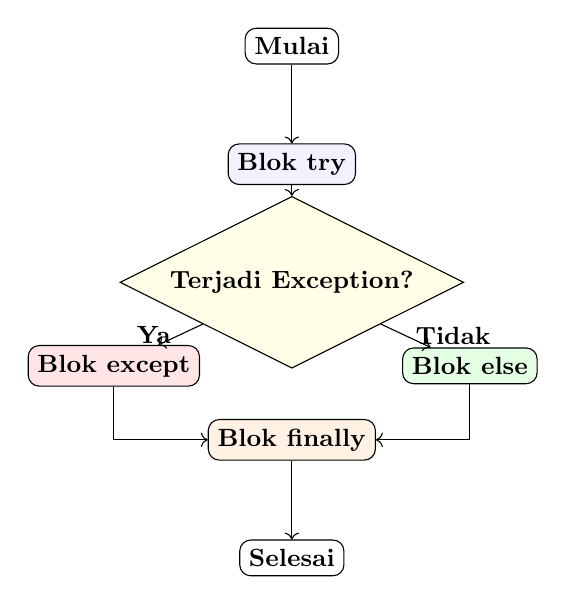
\begin{tikzpicture}[node distance=1.5cm, font=\small, align=center]
\node (start) [draw, rounded corners] {\textbf{Mulai}};
\node (try) [below of=start, draw, rounded corners, fill=blue!5] {\textbf{Blok try}};
\node (error?) [below of=try, draw, diamond, aspect=2, fill=yellow!10] {\textbf{Terjadi Exception?}};
\node (except) [below left of=error?, xshift=-1.2cm, draw, rounded corners, fill=red!10] {\textbf{Blok except}};
\node (else) [below right of=error?, xshift=1.2cm, draw, rounded corners, fill=green!10] {\textbf{Blok else}};
\node (finally) [below of=error?, yshift=-.5cm, draw, rounded corners, fill=orange!10] {\textbf{Blok finally}};
\node (end) [below of=finally, draw, rounded corners] {\textbf{Selesai}};

\draw[->] (start) -- (try);
\draw[->] (try) -- (error?);
\draw[->] (error?) -- node[left]{\textbf{Ya}} (except);
\draw[->] (error?) -- node[right]{\textbf{Tidak}} (else);
\draw[->] (except) |- (finally);
\draw[->] (else) |- (finally);
\draw[->] (finally) -- (end);
\end{tikzpicture}
\end{center}

Diagram di atas menunjukkan bahwa blok \texttt{finally} selalu dijalankan, baik ada exception maupun tidak.

\subsection*{Kesimpulan}

Blok \texttt{else} dan \texttt{finally} membantu kita menulis kode Python yang lebih rapi, aman, dan terstruktur:
\begin{itemize}
    \item Gunakan \texttt{else} untuk kode yang hanya perlu dijalankan jika tidak ada error.
    \item Gunakan \texttt{finally} untuk tindakan pembersihan yang wajib dilakukan.
\end{itemize}

Kombinasi empat blok ini — \texttt{try}, \texttt{except}, \texttt{else}, dan \texttt{finally} — memberi kendali penuh terhadap perilaku program dalam menghadapi kesalahan dan proses penyelesaian.


\section{Membuat Exception Sendiri}

Selain menggunakan berbagai jenis exception bawaan Python seperti \texttt{ValueError} atau \texttt{ZeroDivisionError}, kita juga dapat membuat jenis exception kita sendiri yang sesuai dengan kebutuhan program. Kemampuan ini berguna ketika kita ingin mendefinisikan kesalahan yang bersifat lebih spesifik dan bermakna sesuai konteks aplikasi yang kita kembangkan.

\subsection*{Pengenalan Custom Exception}

\textbf{Custom exception} atau pengecualian buatan sendiri memungkinkan kita membuat tipe kesalahan baru dengan pesan dan perilaku yang kita tentukan. Biasanya, custom exception digunakan untuk situasi yang tidak tercakup oleh exception standar Python.

Sebagai contoh, dalam sebuah aplikasi keuangan, kita mungkin ingin membuat kesalahan khusus seperti \texttt{SaldoTidakCukupError} atau \texttt{TransaksiTidakValidError}. Hal ini membuat kode lebih mudah dibaca dan dipahami, karena jenis error langsung menggambarkan konteks masalahnya.

\subsection*{Cara Mendefinisikan Class Exception Sendiri}

Untuk membuat exception baru, kita cukup mendefinisikan kelas Python yang diturunkan (\textit{inherit}) dari kelas dasar \texttt{Exception}. Kita juga dapat menambahkan konstruktor khusus atau atribut tambahan sesuai kebutuhan.

\begin{lstlisting}[style=PythonStyle, caption={Contoh mendefinisikan custom exception sederhana}]
class InputNegatifError(Exception):
    """Exception yang muncul jika input bernilai negatif."""
    pass

# Contoh penggunaan
def hitung_akar(x):
    if x < 0:
        raise InputNegatifError("Tidak bisa menghitung akar dari bilangan negatif!")
    return x ** 0.5

try:
    angka = int(input("Masukkan angka: "))
    print("Hasil akar:", hitung_akar(angka))
except InputNegatifError as e:
    print("Terjadi kesalahan:", e)
\end{lstlisting}

Ketika pengguna memasukkan angka negatif, hasilnya akan seperti berikut:

\begin{lstlisting}[language=bash]
Masukkan angka: -9
Terjadi kesalahan: Tidak bisa menghitung akar dari bilangan negatif!
\end{lstlisting}

Dalam contoh ini, kita menggunakan \texttt{raise} untuk “melempar” exception buatan sendiri ketika kondisi tidak valid terdeteksi.  
Mekanisme ini sangat berguna untuk mengendalikan alur logika program secara terstruktur.

\subsection*{Menambahkan Atribut dan Konstruktor Khusus}

Kita juga dapat menambahkan informasi tambahan pada exception buatan sendiri, misalnya nilai input yang menyebabkan error, atau pesan khusus yang dapat diproses lebih lanjut.

\begin{lstlisting}[style=PythonStyle, caption={Custom exception dengan atribut tambahan}]
class NilaiTidakValidError(Exception):
    """Exception untuk nilai yang berada di luar rentang tertentu."""
    def __init__(self, nilai, pesan="Nilai di luar rentang yang diperbolehkan."):
        self.nilai = nilai
        self.pesan = pesan
        super().__init__(self.pesan)

def set_nilai(nilai):
    if nilai < 0 or nilai > 100:
        raise NilaiTidakValidError(nilai)
    print(f"Nilai {nilai} disimpan dengan sukses.")

try:
    set_nilai(150)
except NilaiTidakValidError as e:
    print(f"Error: {e.pesan} (nilai: {e.nilai})")
\end{lstlisting}

Keluaran program:

\begin{lstlisting}[language=bash]
Error: Nilai di luar rentang yang diperbolehkan. (nilai: 150)
\end{lstlisting}

Dengan menambahkan atribut seperti \texttt{nilai}, kita dapat melacak konteks kesalahan dengan lebih detail.

\subsection*{Studi Kasus: Validasi Input Pengguna}

Sebagai ilustrasi penerapan nyata, perhatikan contoh berikut: kita akan membuat sistem sederhana yang meminta pengguna memasukkan usia. Program harus menolak nilai yang tidak masuk akal, seperti angka negatif atau usia lebih dari 120 tahun, dengan menggunakan custom exception.

\begin{lstlisting}[style=PythonStyle, caption={Studi kasus: validasi input usia dengan custom exception}]
class UsiaTidakValidError(Exception):
    """Exception untuk usia yang tidak logis."""
    def __init__(self, usia, pesan="Usia tidak valid."):
        self.usia = usia
        self.pesan = pesan
        super().__init__(self.pesan)

def input_usia():
    usia = int(input("Masukkan usia Anda: "))
    if usia < 0:
        raise UsiaTidakValidError(usia, "Usia tidak boleh negatif.")
    elif usia > 120:
        raise UsiaTidakValidError(usia, "Usia terlalu besar untuk manusia.")
    return usia

try:
    umur = input_usia()
    print("Usia Anda adalah:", umur)
except UsiaTidakValidError as e:
    print(f"Error: {e.pesan} (diberikan: {e.usia})")
except ValueError:
    print("Error: Input harus berupa angka.")
\end{lstlisting}

Keluaran contoh:

\begin{lstlisting}[language=bash]
Masukkan usia Anda: -5
Error: Usia tidak boleh negatif. (diberikan: -5)
\end{lstlisting}

Atau:

\begin{lstlisting}[language=bash]
Masukkan usia Anda: 130
Error: Usia terlalu besar untuk manusia. (diberikan: 130)
\end{lstlisting}

Dan jika pengguna memasukkan nilai yang valid:

\begin{lstlisting}[language=bash]
Masukkan usia Anda: 25
Usia Anda adalah: 25
\end{lstlisting}

\subsection*{Manfaat Membuat Exception Sendiri}

Dengan menggunakan custom exception, kita mendapatkan beberapa keuntungan penting:
\begin{itemize}
    \item Kode lebih mudah dibaca karena jenis error menggambarkan konteks spesifik masalah.
    \item Memisahkan kesalahan logika bisnis dari error teknis bawaan Python.
    \item Memudahkan proses debugging dan pelaporan error.
    \item Meningkatkan fleksibilitas dalam menangani kondisi yang tidak biasa.
\end{itemize}

\subsection*{Kesimpulan}

Custom exception memberi kemampuan bagi pengembang untuk mendefinisikan kesalahan sesuai kebutuhan domain aplikasinya.  
Dengan mendefinisikan kelas exception sendiri, kita dapat membuat program yang lebih \textit{robust}, mudah dipelihara, dan kaya informasi saat terjadi kesalahan.

Pada bagian berikutnya, kita akan memperluas topik ini dengan membahas konsep penting berikutnya dalam pengembangan perangkat lunak yang andal — yaitu \textbf{pengujian unit (unit testing)} menggunakan modul \texttt{unittest}.



\section{Latihan}

Bagian ini bertujuan untuk membantu Anda berlatih memahami dan menerapkan konsep \textbf{penanganan kesalahan (exception handling)} dalam Python.  
Setiap soal dirancang untuk memperkuat pemahaman Anda terhadap berbagai aspek seperti penggunaan \texttt{try-except}, \texttt{else}, \texttt{finally}, serta pembuatan \textit{custom exception}.

\subsection*{Latihan Dasar}

\begin{enumerate}
    \item \textbf{Menangani Pembagian Nol}  
    Buatlah sebuah program yang meminta dua input angka dari pengguna dan menampilkan hasil pembagian dari keduanya.  
    Gunakan blok \texttt{try-except} untuk menangani kesalahan \texttt{ZeroDivisionError}.  
    Jika pengguna memasukkan nol sebagai penyebut, tampilkan pesan:  
    \texttt{"Error: Pembagian dengan nol tidak diperbolehkan."}

    \item \textbf{Validasi Input Angka}  
    Tulis program yang meminta pengguna memasukkan sebuah angka bulat.  
    Jika input bukan angka, tangkap kesalahan \texttt{ValueError} dan tampilkan pesan kesalahan yang ramah.  
    Gunakan \texttt{else} untuk mencetak nilai yang berhasil dimasukkan.

    \item \textbf{Membaca File dengan Aman}  
    Buat program yang mencoba membaca isi file berdasarkan nama yang dimasukkan pengguna.  
    Tangani kemungkinan kesalahan \texttt{FileNotFoundError}, dan gunakan \texttt{finally} untuk menampilkan pesan:  
    \texttt{"Operasi selesai, terima kasih."}
\end{enumerate}

\subsection*{Latihan Menengah}

\begin{enumerate}
    \item \textbf{Menangani Beberapa Jenis Exception}  
    Buat program yang meminta pengguna memasukkan dua angka, lalu melakukan operasi pembagian.  
    Tangani dua kemungkinan error:
    \begin{itemize}
        \item \texttt{ValueError} – jika pengguna tidak memasukkan angka.
        \item \texttt{ZeroDivisionError} – jika penyebut bernilai nol.
    \end{itemize}
    Tambahkan blok \texttt{else} untuk mencetak hasil jika tidak ada kesalahan, dan blok \texttt{finally} untuk menampilkan pesan “Selesai memproses data.”

    \item \textbf{Membuat Custom Exception}  
    Buat kelas exception baru bernama \texttt{NilaiNegatifError} yang muncul jika input pengguna berupa angka negatif.  
    Gunakan exception ini dalam fungsi \texttt{cek\_positif(n)} yang akan menolak angka negatif dengan pesan error:  
    \texttt{"Nilai tidak boleh negatif!"}  
    Tampilkan contoh penggunaan fungsi ini dalam blok \texttt{try-except}.
\end{enumerate}

\subsection*{Tantangan Lanjutan}

\begin{enumerate}
    \item \textbf{Validasi Formulir Sederhana}  
    Buat program yang mensimulasikan pengisian formulir dengan tiga input:
    \begin{itemize}
        \item Nama (tidak boleh kosong),
        \item Usia (harus antara 0–120),
        \item Email (harus mengandung karakter '@').
    \end{itemize}
    Buat tiga \textit{custom exception}:
    \begin{itemize}
        \item \texttt{NamaKosongError},
        \item \texttt{UsiaTidakValidError},
        \item \texttt{EmailTidakValidError}.
    \end{itemize}
    Gunakan ketiga exception tersebut untuk memvalidasi data pengguna dan tampilkan pesan kesalahan yang sesuai jika ada input yang tidak valid.

    \item \textbf{Simulasi ATM Sederhana}  
    Buat program simulasi ATM dengan fitur:
    \begin{itemize}
        \item Pengguna dapat memasukkan saldo awal.
        \item Pengguna dapat melakukan penarikan sejumlah uang.
    \end{itemize}
    Buat exception baru bernama \texttt{SaldoTidakCukupError} yang muncul jika pengguna mencoba menarik saldo lebih besar dari jumlah yang tersedia.  
    Gunakan blok \texttt{try-except-finally} untuk menampilkan pesan saldo akhir meskipun terjadi kesalahan.

    \item \textbf{Menangkap dan Menulis Log Kesalahan}  
    Buat program yang menjalankan beberapa operasi aritmetika dari daftar, seperti pembagian, akar kuadrat, dan konversi tipe data.  
    Jika terjadi exception, tangkap semua jenis kesalahan (\texttt{Exception}) dan tulis pesan error ke file bernama \texttt{error.log}.  
    Setiap baris log harus memuat waktu kejadian dan jenis error yang terjadi.
\end{enumerate}

\subsection*{Refleksi}

Setelah menyelesaikan latihan di atas, renungkan pertanyaan berikut:
\begin{itemize}
    \item Mengapa penting untuk menangani kesalahan secara eksplisit?
    \item Dalam situasi apa sebaiknya kita menggunakan custom exception?
    \item Bagaimana penanganan exception dapat meningkatkan pengalaman pengguna (\textit{user experience})?
\end{itemize}

Latihan-latihan ini diharapkan dapat membantu Anda memahami konsep dasar hingga lanjutan dari penanganan kesalahan, serta menyiapkan landasan kuat sebelum mempelajari topik selanjutnya: \textbf{pengujian unit (unit testing)}.


\section{Ringkasan}

Pada bab ini, Anda telah mempelajari bahwa kesalahan (\textit{error}) adalah bagian alami dari pemrograman dan dapat ditangani secara elegan menggunakan mekanisme \textbf{exception}. Kita membedakan antara \textit{syntax error} (terdeteksi sebelum eksekusi) dan \textit{runtime error}/\textbf{exception} (muncul saat program berjalan). Dengan blok \texttt{try-except}, alur program tidak perlu terhenti; Anda dapat memberikan pesan yang ramah, mengambil tindakan pemulihan, dan menjaga pengalaman pengguna. Kita juga meninjau pola lanjut seperti \texttt{else} (dijalankan saat tidak ada error) dan \texttt{finally} (selalu dijalankan untuk \textit{cleanup}), serta menangani banyak jenis exception secara spesifik agar debugging lebih mudah dan kode lebih jelas. Selain itu, Anda belajar membuat \textbf{custom exception} untuk mengekspresikan aturan bisnis/domain secara eksplisit.

Fondasi ini menjadi pasangan erat bagi praktik \textbf{pengujian} dalam pengembangan perangkat lunak yang andal. Dengan pemahaman exception handling yang kuat, Anda siap melangkah ke pengujian otomatis (misalnya dengan \texttt{unittest}) guna memverifikasi perilaku fungsi, mencegah regresi, dan mempertahankan kualitas kode seiring perubahan. Intinya: gunakan \texttt{try-except-else-finally} untuk mengendalikan alur saat terjadi kondisi tak terduga, manfaatkan exception yang spesifik (atau custom) untuk kejelasan, dan lengkapi dengan pengujian yang baik agar program tetap \textit{robust}, mudah dirawat, dan dapat diandalkan.

	%========================================================
% CHAPTER: Unit Test di Python
%========================================================
\chapter{Unit Test di Python}
\label{ch:unit-test-python}


%----------------------------------------
\section{Pendahuluan}

Unit testing atau pengujian unit merupakan salah satu tahap penting dalam proses pengembangan perangkat lunak. Pada dasarnya, unit test bertujuan untuk memastikan bahwa setiap bagian kecil dari program — biasanya berupa fungsi atau method — bekerja sesuai dengan yang diharapkan. Dengan melakukan pengujian sejak tahap paling awal, kesalahan logika dapat ditemukan lebih cepat sebelum kode bergabung dengan komponen lain yang lebih kompleks.

\subsection{Mengapa Unit Test Penting}

Unit test penting karena beberapa alasan utama berikut:

\begin{enumerate}
    \item \textbf{Deteksi dini kesalahan.}  
    Kesalahan logika atau bug dapat ditemukan lebih awal, bahkan sebelum kode diintegrasikan dengan modul lain.
    
    \item \textbf{Meningkatkan kepercayaan diri saat refactoring.}  
    Ketika kode diubah atau disempurnakan, unit test yang telah ada akan memastikan bahwa perilaku lama tetap konsisten dan tidak terjadi regresi.
    
    \item \textbf{Mendukung dokumentasi fungsional.}  
    Unit test berfungsi sebagai contoh nyata bagaimana fungsi atau method seharusnya digunakan dan apa hasil yang diharapkan.
    
    \item \textbf{Mempercepat proses pengembangan jangka panjang.}  
    Walaupun menulis test membutuhkan waktu di awal, pengujian otomatis akan menghemat waktu debugging di masa depan.
    
    \item \textbf{Menjadi dasar untuk integrasi dan pengujian lanjutan.}  
    Unit test adalah pondasi untuk pengujian tingkat lebih tinggi seperti integration test dan end-to-end test.
\end{enumerate}

Dengan kata lain, unit test memberikan jaminan bahwa setiap “unit terkecil” dari program dapat berdiri sendiri dan berfungsi sesuai kontrak yang didefinisikan oleh pengembang.

\subsection{Prinsip Dasar Pengujian Unit}

Dalam praktiknya, pengujian unit mengikuti beberapa prinsip dasar yang membuat test efektif, dapat diandalkan, dan mudah dipelihara:

\begin{itemize}
    \item \textbf{Isolasi.}  
    Setiap test harus menguji satu fungsi atau method secara terpisah, tanpa bergantung pada hasil dari test lain.
    
    \item \textbf{Deterministik.}  
    Test harus menghasilkan hasil yang sama setiap kali dijalankan, terlepas dari urutan eksekusi atau kondisi eksternal.
    
    \item \textbf{Kemandirian.}  
    Test tidak boleh bergantung pada database, jaringan, atau file eksternal kecuali benar-benar diperlukan.
    
    \item \textbf{Repeatability.}  
    Unit test harus dapat dijalankan berulang kali dengan hasil yang konsisten, baik secara lokal maupun di lingkungan CI/CD.
    
    \item \textbf{FAST (First, Automated, Small, Testable).}  
    Unit test idealnya cepat, mudah dijalankan otomatis, berfokus pada bagian kecil kode, dan mudah diperluas.
\end{itemize}

Dengan memahami prinsip-prinsip ini, pengembang dapat menulis unit test yang sederhana, efektif, dan mudah dirawat.  
Pada bab ini, kita akan fokus pada pengujian fungsi dan method menggunakan modul bawaan Python, yaitu \texttt{unittest}.


%----------------------------------------
\section{Pengenalan Modul \texttt{unittest}}

Python menyediakan modul bawaan bernama \texttt{unittest} yang digunakan untuk menulis dan menjalankan pengujian unit. Modul ini sudah termasuk dalam instalasi standar Python, sehingga tidak memerlukan instalasi tambahan seperti pustaka pihak ketiga (\textit{third-party library}).  
\texttt{unittest} terinspirasi dari kerangka kerja \textit{xUnit}, yaitu gaya pengujian berorientasi objek yang juga digunakan dalam bahasa lain seperti Java (\texttt{JUnit}) dan C\# (\texttt{NUnit}).

Modul ini menyediakan serangkaian kelas dan metode yang membantu pengembang:
\begin{itemize}
    \item mendefinisikan \textit{test case} (kasus uji) dalam bentuk kelas,
    \item melakukan pengecekan hasil dengan berbagai \textit{assertion},
    \item mengelompokkan beberapa test menjadi satu \textit{test suite},
    \item serta menjalankan semua test secara otomatis.
\end{itemize}

\subsection{Struktur Dasar \texttt{TestCase}}

Setiap unit test pada Python biasanya ditulis sebagai sebuah kelas yang menurunkan (\texttt{inherit}) dari kelas \texttt{unittest.TestCase}.  
Di dalam kelas tersebut, setiap metode yang namanya diawali dengan \texttt{test\_} akan dianggap sebagai sebuah test case oleh kerangka kerja \texttt{unittest}.

Secara umum, struktur dasar test dalam \texttt{unittest} terdiri dari:

\begin{enumerate}
    \item \textbf{Import modul \texttt{unittest}.}  
    Langkah pertama adalah mengimpor modul \texttt{unittest} ke dalam berkas Python.

    \item \textbf{Membuat kelas turunan dari \texttt{unittest.TestCase}.}  
    Kelas ini akan menampung satu atau lebih metode pengujian yang akan dijalankan.

    \item \textbf{Menulis metode pengujian dengan nama diawali \texttt{test\_}.}  
    Setiap metode mewakili satu skenario uji tertentu.  
    Di dalamnya, kita menggunakan metode \texttt{assert*} untuk membandingkan hasil aktual dan hasil yang diharapkan.

    \item \textbf{Menjalankan test.}  
    Test dapat dijalankan langsung melalui perintah \texttt{python -m unittest} dari terminal, atau dengan menambahkan blok standar:
\end{enumerate}

\begin{lstlisting}[style=PythonStyle, caption={Blok eksekusi test bawaan}, label={lst:main-block}]
if __name__ == "__main__":
    unittest.main()
\end{lstlisting}

Contoh sederhana strukturnya dapat dijelaskan sebagai berikut (placeholder tanpa isi fungsi):

\begin{lstlisting}[style=PythonStyle, caption={Struktur dasar kelas unit test di Python}, label={lst:unittest-structure}]
import unittest

class TestNamaFungsi(unittest.TestCase):
    def test_kasus_1(self):
        # TODO: tulis logika pengujian
        self.assertEqual(1 + 1, 2)

if __name__ == "__main__":
    unittest.main()
\end{lstlisting}

Ketika program dijalankan, kerangka \texttt{unittest} akan mencari semua kelas turunan dari \texttt{unittest.TestCase} dan mengeksekusi setiap metode yang diawali dengan \texttt{test\_}.  
Setiap test akan dilaporkan hasilnya dalam format:
\begin{itemize}
    \item \texttt{.} (titik) → test berhasil (\textit{passed}),
    \item \texttt{F} → test gagal (\textit{failed}),
    \item \texttt{E} → terjadi error selama eksekusi test.
\end{itemize}

\subsection{Menjalankan Test}

Setelah test dibuat, ada beberapa cara untuk menjalankannya menggunakan modul \texttt{unittest}:

\begin{enumerate}
    \item \textbf{Menjalankan langsung dari berkas Python.}  
    Jika test disimpan dalam file seperti \texttt{test\_fungsi.py}, maka jalankan:
    \begin{lstlisting}[language=bash]
    python test_fungsi.py
    \end{lstlisting}
    Blok \texttt{if \_\_name\_\_ == "\_\_main\_\_"} memastikan test otomatis berjalan saat file dijalankan secara langsung.

    \item \textbf{Menggunakan perintah bawaan \texttt{unittest}.}  
    Jalankan semua test dalam satu direktori menggunakan:
    \begin{lstlisting}[language=bash]
    python -m unittest discover
    \end{lstlisting}
    Perintah ini akan mencari seluruh berkas dengan pola nama \texttt{test\_*.py} atau \texttt{*\_test.py} dan mengeksekusinya.

    \item \textbf{Menjalankan test tertentu saja.}  
    Jika hanya ingin menjalankan satu test case atau metode tertentu:
    \begin{lstlisting}[language=bash]
    python -m unittest test_fungsi.TestNamaFungsi.test_kasus_1
    \end{lstlisting}

    \item \textbf{Menambah tingkat keluaran (verbosity).}  
    Gunakan opsi \texttt{-v} untuk menampilkan nama test dan status hasil secara lebih rinci:
    \begin{lstlisting}[language=bash]
    python -m unittest -v
    \end{lstlisting}
\end{enumerate}

Hasil eksekusi akan menampilkan laporan yang mudah dibaca, misalnya:

\begin{lstlisting}[language=bash]
test_kasus_1 (test_fungsi.TestNamaFungsi) ... ok

----------------------------------------------------------------------
Ran 1 test in 0.001s

OK
\end{lstlisting}

Dengan memahami struktur dasar dan cara menjalankan test ini, pengembang sudah dapat mulai menulis dan mengeksekusi unit test untuk fungsi dan method di proyek Python apa pun tanpa memerlukan pustaka tambahan.


%----------------------------------------
\section{Menulis Unit Test untuk Fungsi}

Pada tahap ini, kita akan mempelajari cara menulis pengujian unit untuk sebuah fungsi Python menggunakan modul bawaan \texttt{unittest}.  
Pengujian terhadap fungsi merupakan bentuk paling sederhana dari unit test karena fungsi biasanya menerima sejumlah argumen, melakukan perhitungan atau logika tertentu, dan mengembalikan hasil yang dapat diuji secara deterministik.

\subsection{Langkah-langkah Dasar}

Langkah-langkah umum untuk menulis unit test pada fungsi adalah sebagai berikut:

\begin{enumerate}
    \item \textbf{Tuliskan fungsi yang akan diuji.}  
    Buat fungsi di berkas Python terpisah (misalnya \texttt{fungsi.py}).  
    Fungsi sebaiknya memiliki perilaku yang jelas dan hasil yang dapat diprediksi untuk input tertentu.

    \item \textbf{Buat berkas test terpisah.}  
    Umumnya file test diberi nama dengan awalan \texttt{test\_}, misalnya \texttt{test\_fungsi.py}.  
    File ini berisi kode pengujian yang menggunakan modul \texttt{unittest}.

    \item \textbf{Import fungsi yang akan diuji.}  
    Di dalam file test, impor fungsi dari modul utama agar dapat diuji.

    \item \textbf{Buat kelas turunan dari \texttt{unittest.TestCase}.}  
    Kelas ini berisi metode yang masing-masing mewakili satu kasus uji.

    \item \textbf{Gunakan metode \texttt{assert*} untuk membandingkan hasil aktual dan ekspektasi.}  
    Contoh metode \texttt{assert*} yang sering digunakan:  
    \texttt{assertEqual}, \texttt{assertTrue}, \texttt{assertFalse}, dan \texttt{assertRaises}.

    \item \textbf{Jalankan test dan periksa hasilnya.}  
    Gunakan perintah:
    \begin{lstlisting}[language=bash]
    python -m unittest test_fungsi.py
    \end{lstlisting}
\end{enumerate}

Dengan mengikuti enam langkah tersebut, Anda dapat menguji fungsi apa pun yang memiliki input dan output yang terdefinisi dengan baik.

\subsection{Contoh Placeholder}

Berikut contoh sederhana fungsi dan pengujiannya.  
Misalkan kita memiliki fungsi \texttt{add(a, b)} yang bertugas menjumlahkan dua bilangan.

\begin{lstlisting}[style=PythonStyle, caption={Fungsi yang akan diuji}, label={lst:fungsi-add}]
# file: fungsi.py
def add(a, b):
    """Menjumlahkan dua bilangan dan mengembalikan hasilnya."""
    return a + b
\end{lstlisting}

Kemudian, kita buat berkas terpisah untuk pengujian unitnya:

\begin{lstlisting}[style=PythonStyle, caption={Contoh pengujian fungsi sederhana}, label={lst:test-fungsi}]
# file: test_fungsi.py
import unittest
from fungsi import add   # mengimpor fungsi yang akan diuji

class TestAddFunction(unittest.TestCase):
    def test_penjumlahan_positif(self):
        self.assertEqual(add(2, 3), 5)

    def test_penjumlahan_negatif(self):
        self.assertEqual(add(-4, -6), -10)

    def test_penjumlahan_nol(self):
        self.assertEqual(add(0, 0), 0)

if __name__ == "__main__":
    unittest.main()
\end{lstlisting}

Untuk menjalankan pengujian, gunakan perintah:

\begin{lstlisting}[language=bash]
python -m unittest test_fungsi.py
\end{lstlisting}

Keluaran yang diharapkan:

\begin{lstlisting}[language=bash]
...
----------------------------------------------------------------------
Ran 3 tests in 0.001s

OK
\end{lstlisting}

Dalam contoh di atas:
\begin{itemize}
    \item Tiga metode pengujian menguji tiga skenario berbeda untuk fungsi yang sama.
    \item Jika salah satu hasil tidak sesuai dengan ekspektasi, \texttt{unittest} akan menampilkan huruf \texttt{F} (fail) dan memberikan pesan perbandingan nilai aktual vs. nilai yang diharapkan.
    \item Kode ini bisa dijalankan berulang kali tanpa ketergantungan eksternal.
\end{itemize}

Pendekatan ini dapat digunakan untuk menguji berbagai fungsi lain seperti konversi nilai, validasi input, maupun operasi matematis sederhana.  
Intinya, setiap fungsi yang memiliki hasil pasti untuk input tertentu dapat dan sebaiknya memiliki \textit{unit test}.

%----------------------------------------
\section{Menulis Unit Test untuk Method di Kelas}

Pengujian method pada kelas serupa dengan pengujian fungsi, namun sering kali melibatkan \emph{state} objek (atribut instance) dan berbagai jenis method (instance, \texttt{@staticmethod}, \texttt{@classmethod}).  
Bagian ini menunjukkan pola umum untuk masing-masing jenis method serta cara menggunakan \texttt{setUp}/\texttt{tearDown} untuk menyiapkan dan membersihkan objek uji.

\subsection{Menguji Method Biasa (Instance Method)}

\textbf{Instance method} bergantung pada state objek (\texttt{self}).  
Pola umum pengujiannya:
\begin{enumerate}
    \item Buat instance objek pada awal test (dengan \texttt{setUp} atau langsung di metode test).
    \item Panggil method yang diuji dengan argumen yang relevan.
    \item Gunakan \texttt{assert*} untuk memeriksa hasil.
    \item Jika method dapat memunculkan error pada kondisi tertentu, gunakan \texttt{assertRaises}.
\end{enumerate}

\subsection{Menguji Method Static dan Classmethod}

\textbf{Static method} tidak bergantung pada state objek atau kelas; ia berperilaku seperti fungsi biasa yang ditempatkan di dalam kelas.  
\textbf{Class method} menerima \texttt{cls} sebagai argumen pertama dan lazim digunakan sebagai \emph{alternate constructor} atau operasi yang logis pada tingkat kelas.  
Keduanya diuji dengan memanggilnya via \texttt{NamaKelas.method(...)} atau melalui instance.

\subsection{Menggunakan \texttt{setUp} dan \texttt{tearDown}}

Gunakan \texttt{setUp} untuk menyiapkan objek/lingkungan sebelum setiap test case dijalankan, dan \texttt{tearDown} untuk membersihkan setelahnya.  
Hal ini memastikan setiap test berjalan dalam kondisi yang segar (\emph{fresh}) dan terisolasi.

\begin{lstlisting}[style=PythonStyle, caption={Kode kelas contoh untuk diuji}, label={lst:calculator-impl}]
# file: calculator.py

class Calculator:
    def __init__(self, memory: float = 0.0):
        # state internal: menyimpan nilai terakhir
        self.memory = float(memory)

    # -------- Instance methods --------
    def add(self, a: float, b: float) -> float:
        """Menjumlahkan a dan b, memperbarui memory, dan mengembalikan hasil."""
        result = float(a) + float(b)
        self.memory = result
        return result

    def divide(self, a: float, b: float) -> float:
        """Membagi a dengan b. Memunculkan ZeroDivisionError jika b == 0."""
        if b == 0:
            raise ZeroDivisionError("pembagian dengan nol")
        result = float(a) / float(b)
        self.memory = result
        return result

    # -------- Static method --------
    @staticmethod
    def is_even(n: int) -> bool:
        """Mengembalikan True jika n genap, False jika ganjil."""
        return (n % 2) == 0

    # -------- Class method --------
    @classmethod
    def from_string(cls, s: str) -> "Calculator":
        """
        Alternate constructor: membuat Calculator dari string angka.
        Jika string tidak valid, ValueError.
        """
        try:
            val = float(s.strip())
        except Exception as e:
            raise ValueError(f"nilai tidak valid: {s}") from e
        return cls(memory=val)
\end{lstlisting}

\begin{lstlisting}[style=PythonStyle, caption={Pengujian method kelas dengan unittest}, label={lst:test-method}]
# file: test_calculator.py
import unittest
from calculator import Calculator

class TestCalculatorMethods(unittest.TestCase):
    def setUp(self):
        # Dipanggil sebelum setiap test_*
        # Siapkan objek baru agar setiap test terisolasi
        self.calc = Calculator()

    def tearDown(self):
        # Dipanggil setelah setiap test_*
        # Biasanya untuk cleanup resource; di sini cukup reset referensi
        self.calc = None

    # ---------- Instance methods ----------
    def test_add_mengembalikan_hasil_dan_update_memory(self):
        hasil = self.calc.add(2, 3)
        self.assertEqual(hasil, 5.0)
        self.assertEqual(self.calc.memory, 5.0)

    def test_divide_normal(self):
        hasil = self.calc.divide(10, 2)
        self.assertEqual(hasil, 5.0)
        self.assertEqual(self.calc.memory, 5.0)

    def test_divide_zero_raises(self):
        with self.assertRaises(ZeroDivisionError):
            self.calc.divide(1, 0)

    # SubTest untuk variasi input add
    def test_add_dengan_variansi_input(self):
        kasus = [
            (0, 0, 0.0),
            (1, -1, 0.0),
            (2.5, 0.5, 3.0),
            (-3, -7, -10.0),
        ]
        for a, b, expected in kasus:
            with self.subTest(a=a, b=b):
                self.assertEqual(self.calc.add(a, b), expected)

    # ---------- Static method ----------
    def test_is_even(self):
        # Bisa dipanggil via kelas atau instance
        self.assertTrue(Calculator.is_even(2))
        self.assertFalse(self.calc.is_even(3))

    # ---------- Class method ----------
    def test_from_string_valid(self):
        c = Calculator.from_string("  42.5 ")
        self.assertIsInstance(c, Calculator)
        self.assertEqual(c.memory, 42.5)

    def test_from_string_invalid_raises(self):
        with self.assertRaises(ValueError):
            Calculator.from_string("bukan-angka")

if __name__ == "__main__":
    unittest.main()
\end{lstlisting}

Untuk menjalankan pengujian:

\begin{lstlisting}[language=bash]
python -m unittest test_calculator.py
\end{lstlisting}

\noindent
Keluaran yang diharapkan (ilustrasi):

\begin{lstlisting}[language=bash]
test_add_dengan_variansi_input (test_calculator.TestCalculatorMethods) ... ok
test_add_mengembalikan_hasil_dan_update_memory (test_calculator.TestCalculatorMethods) ... ok
test_divide_normal (test_calculator.TestCalculatorMethods) ... ok
test_divide_zero_raises (test_calculator.TestCalculatorMethods) ... ok
test_from_string_invalid_raises (test_calculator.TestCalculatorMethods) ... ok
test_from_string_valid (test_calculator.TestCalculatorMethods) ... ok
test_is_even (test_calculator.TestCalculatorMethods) ... ok

----------------------------------------------------------------------
Ran 7 tests in 0.00Xs

OK
\end{lstlisting}

Penekanan utama dari contoh di atas:
\begin{itemize}
    \item \textbf{Instance method} diuji baik untuk hasil benar maupun skenario error (\texttt{assertRaises}).
    \item \textbf{Static method} diuji seperti fungsi murni yang tidak bergantung state.
    \item \textbf{Class method} diuji sebagai \emph{alternate constructor} untuk memastikan validasi input berjalan.
    \item \textbf{\texttt{setUp}/\texttt{tearDown}} memastikan setiap test berjalan di lingkungan yang bersih.
    \item \textbf{\texttt{subTest}} dipakai untuk menguji banyak variasi input tanpa menulis metode test terpisah.
\end{itemize}

%----------------------------------------
\section{Assertion Dasar dalam \texttt{unittest}}

Dalam modul \texttt{unittest}, pengujian dilakukan dengan memeriksa apakah hasil aktual dari suatu fungsi atau method sesuai dengan nilai yang diharapkan.  
Pemeriksaan ini dilakukan menggunakan berbagai metode \textit{assertion} yang disediakan oleh kelas \texttt{unittest.TestCase}.  
Setiap metode assertion akan menandai test sebagai \textit{failed} apabila kondisi yang diuji tidak terpenuhi, dan menampilkan pesan perbandingan antara hasil aktual dan ekspektasi.

Secara umum, assertion berperan sebagai “kontrak” atau “pernyataan kebenaran” yang harus selalu valid bagi fungsi yang diuji.

\subsection{\texttt{assertEqual}, \texttt{assertTrue}, \texttt{assertFalse}}

Tiga metode ini adalah yang paling sering digunakan dalam unit test sederhana.

\begin{itemize}
    \item \texttt{assertEqual(a, b)} — memastikan bahwa dua nilai sama persis.
    \item \texttt{assertTrue(expr)} — memastikan bahwa ekspresi bernilai benar.
    \item \texttt{assertFalse(expr)} — memastikan bahwa ekspresi bernilai salah.
\end{itemize}

Jika kondisi tidak terpenuhi, unittest akan menandai test tersebut sebagai gagal dan mencetak pesan perbandingan nilai aktual vs nilai ekspektasi.

\begin{lstlisting}[style=PythonStyle, caption={Contoh penggunaan assertEqual, assertTrue, dan assertFalse}, label={lst:assert-basic}]
import unittest

def is_even(n: int) -> bool:
    return (n % 2) == 0

def square(x: int) -> int:
    return x * x

class TestAssertionDasar(unittest.TestCase):
    def test_assert_equal(self):
        self.assertEqual(square(3), 9)
        self.assertEqual(square(-4), 16)

    def test_assert_true_false(self):
        self.assertTrue(is_even(2))
        self.assertFalse(is_even(3))

if __name__ == "__main__":
    unittest.main()
\end{lstlisting}

Ketika test dijalankan, hasil yang diharapkan:

\begin{lstlisting}[language=bash]
...
----------------------------------------------------------------------
Ran 2 tests in 0.000s

OK
\end{lstlisting}

Beberapa metode assertion lain yang tersedia antara lain:
\begin{itemize}
    \item \texttt{assertNotEqual(a, b)}
    \item \texttt{assertIsNone(x)}, \texttt{assertIsNotNone(x)}
    \item \texttt{assertIn(member, container)}, \texttt{assertNotIn(member, container)}
    \item \texttt{assertAlmostEqual(a, b, places=n)} — membandingkan dua nilai numerik dengan toleransi desimal tertentu.
\end{itemize}

\subsection{\texttt{assertRaises} untuk Menguji Error}

Terkadang fungsi atau method diharapkan memunculkan error dalam kondisi tertentu.  
Untuk menguji perilaku tersebut, kita dapat menggunakan \texttt{assertRaises}.  
Assertion ini memastikan bahwa exception benar-benar dilempar (raised) saat kode dijalankan.

Ada dua bentuk umum penggunaan:
\begin{enumerate}
    \item \textbf{Sebagai konteks (dengan \texttt{with}).}
    \item \textbf{Sebagai pemanggilan langsung.}
\end{enumerate}

Contoh:

\begin{lstlisting}[style=PythonStyle, caption={Contoh penggunaan assertRaises}, label={lst:assertraises}]
import unittest

def divide(a, b):
    if b == 0:
        raise ZeroDivisionError("pembagian dengan nol tidak diperbolehkan")
    return a / b

class TestErrorHandling(unittest.TestCase):
    def test_divide_normal(self):
        self.assertEqual(divide(10, 2), 5)

    def test_divide_zero(self):
        # Bentuk konteks
        with self.assertRaises(ZeroDivisionError):
            divide(4, 0)

    def test_divide_zero_pakai_lambda(self):
        # Bentuk pemanggilan langsung
        self.assertRaises(ZeroDivisionError, divide, 1, 0)

if __name__ == "__main__":
    unittest.main()
\end{lstlisting}

Ketika dijalankan:

\begin{lstlisting}[language=bash]
...
----------------------------------------------------------------------
Ran 3 tests in 0.001s

OK
\end{lstlisting}

Penggunaan \texttt{assertRaises} penting karena memungkinkan kita menguji skenario negatif — memastikan fungsi tidak hanya bekerja saat benar, tetapi juga gagal dengan cara yang tepat saat kondisi salah terjadi.

\subsection{\texttt{subTest} untuk Menguji Beberapa Kasus}

Jika satu fungsi perlu diuji dengan berbagai kombinasi input, kita bisa menggunakan \texttt{subTest}.  
Fitur ini membantu menjalankan banyak variasi pengujian di dalam satu metode tanpa menghentikan eksekusi setelah satu kasus gagal.

\begin{lstlisting}[style=PythonStyle, caption={Penggunaan subTest untuk beberapa kasus input}, label={lst:subtest}]
import unittest

def multiply(a, b):
    return a * b

class TestSubTest(unittest.TestCase):
    def test_multiply_variatif(self):
        # Beberapa kasus uji dalam satu metode
        kasus = [
            (2, 3, 6),
            (0, 10, 0),
            (-2, 4, -8),
            (1.5, 2, 3.0),
        ]
        for a, b, expected in kasus:
            with self.subTest(a=a, b=b):
                self.assertEqual(multiply(a, b), expected)

if __name__ == "__main__":
    unittest.main()
\end{lstlisting}

Hasil eksekusi:

\begin{lstlisting}[language=bash]
...
----------------------------------------------------------------------
Ran 1 test in 0.000s

OK
\end{lstlisting}

Jika salah satu subTest gagal, laporan akan tetap menampilkan semua kasus dan menunjukkan kombinasi input mana yang menyebabkan kegagalan, contohnya:

\begin{lstlisting}[language=bash]
FAIL: test_multiply_variatif (__main__.TestSubTest) (a=2, b=3)
AssertionError: 5 != 6
\end{lstlisting}

\texttt{subTest} sangat berguna untuk menghemat waktu, meningkatkan keterbacaan test, dan menghindari duplikasi kode pada kasus pengujian yang hanya berbeda data inputnya.

---

Dengan memahami dan mempraktikkan tiga jenis assertion ini — \texttt{assertEqual}/\texttt{assertTrue}/\texttt{assertFalse}, \texttt{assertRaises}, dan \texttt{subTest} — pengembang dapat menulis pengujian yang komprehensif dan mudah dipelihara untuk hampir semua fungsi dan method dalam proyek Python.


%----------------------------------------
\section{Menjalankan dan Membaca Hasil}

Setelah kita menulis berbagai test menggunakan modul \texttt{unittest}, langkah berikutnya adalah menjalankannya dan membaca hasilnya.  
Python menyediakan cara bawaan untuk mengeksekusi test baik secara individual maupun otomatis (melalui *test discovery*).  
Pemahaman terhadap format hasil dan pesan error akan membantu kita mendiagnosis sumber kesalahan dengan cepat.

\subsection{Menjalankan via CLI: \texttt{python -m unittest}}

Cara paling umum untuk menjalankan unit test adalah menggunakan modul \texttt{unittest} melalui perintah baris (Command Line Interface / CLI).

\begin{lstlisting}[language=bash, caption={Menjalankan file test tertentu}]
python -m unittest test_fungsi.py
\end{lstlisting}

Perintah di atas akan menjalankan semua kelas dan metode test yang terdapat di dalam berkas \texttt{test\_fungsi.py}.  
Secara default, hanya test yang namanya diawali dengan \texttt{test\_} yang akan dijalankan.

Selain menjalankan satu file, kita juga dapat:

\begin{itemize}
    \item \textbf{Menjalankan semua test dalam proyek (discovery):}
    \begin{lstlisting}[language=bash]
    python -m unittest discover
    \end{lstlisting}
    Perintah ini akan mencari seluruh berkas dengan pola nama \texttt{test\_*.py} atau \texttt{*\_test.py} di direktori saat ini dan subdirektorinya.

    \item \textbf{Menjalankan test tertentu saja:}
    \begin{lstlisting}[language=bash]
    python -m unittest test_fungsi.TestAddFunction.test_penjumlahan_positif
    \end{lstlisting}
    Berguna untuk mengeksekusi hanya satu test case spesifik tanpa menjalankan semua test lainnya.

    \item \textbf{Menambah tingkat keluaran (verbosity):}
    \begin{lstlisting}[language=bash]
    python -m unittest -v
    \end{lstlisting}
    Opsi \texttt{-v} (\emph{verbose}) akan menampilkan nama setiap test case dan status hasilnya secara lebih rinci.

    \item \textbf{Menjalankan beberapa test sekaligus:}
    \begin{lstlisting}[language=bash]
    python -m unittest test_fungsi test_calculator
    \end{lstlisting}
    Kita dapat mencantumkan beberapa modul test sekaligus dalam satu perintah.
\end{itemize}

Contoh hasil eksekusi dengan opsi verbose:

\begin{lstlisting}[language=bash]
test_penjumlahan_positif (test_fungsi.TestAddFunction) ... ok
test_penjumlahan_negatif (test_fungsi.TestAddFunction) ... ok
test_penjumlahan_nol (test_fungsi.TestAddFunction) ... ok

----------------------------------------------------------------------
Ran 3 tests in 0.001s

OK
\end{lstlisting}

Penjelasan hasil:
\begin{itemize}
    \item \texttt{ok} → Test berhasil.
    \item \texttt{FAIL} → Hasil tidak sesuai ekspektasi.
    \item \texttt{ERROR} → Terjadi error yang tidak ditangani (exception) di luar mekanisme assertion.
\end{itemize}

Dalam mode non-verbose (tanpa \texttt{-v}), simbol yang digunakan lebih ringkas:
\begin{center}
\begin{tabular}{ll}
\texttt{.} & Test berhasil (passed) \\
\texttt{F} & Test gagal (failed) \\
\texttt{E} & Test error (exception tak tertangani) \\
\end{tabular}
\end{center}

\noindent
Contoh output minimal:
\begin{lstlisting}[language=bash]
..F
======================================================================
FAIL: test_penjumlahan_nol (test_fungsi.TestAddFunction)
----------------------------------------------------------------------
Traceback (most recent call last):
  File "test_fungsi.py", line 9, in test_penjumlahan_nol
    self.assertEqual(add(0, 0), 1)
AssertionError: 0 != 1

----------------------------------------------------------------------
Ran 3 tests in 0.000s

FAILED (failures=1)
\end{lstlisting}

\subsection{Menafsirkan Output dan Traceback}

Jika terdapat test yang gagal, \texttt{unittest} akan menampilkan laporan detail berupa *traceback* untuk membantu menemukan penyebab kesalahan.  
Berikut penjelasan struktur laporan tersebut:

\begin{itemize}
    \item \textbf{Nama test yang gagal:}  
    Ditunjukkan dalam baris seperti  
    \texttt{FAIL: test\_penjumlahan\_nol (test\_fungsi.TestAddFunction)}  
    yang berarti metode \texttt{test\_penjumlahan\_nol} di kelas \texttt{TestAddFunction} gagal.

    \item \textbf{Lokasi kesalahan:}  
    Baris berikutnya menunjukkan nama file dan nomor baris, misalnya:  
    \texttt{File "test\_fungsi.py", line 9, in test\_penjumlahan\_nol}

    \item \textbf{Pernyataan assertion yang gagal:}  
    Baris seperti  
    \texttt{AssertionError: 0 != 1}  
    menunjukkan bahwa nilai aktual (0) tidak sama dengan ekspektasi (1).

    \item \textbf{Ringkasan hasil keseluruhan:}  
    Ditampilkan di bagian akhir, misalnya:
\end{itemize}

\begin{lstlisting}[language=bash]
FAILED (failures=1)
\end{lstlisting}

Selain \texttt{FAIL}, mungkin juga muncul status \texttt{ERROR} jika test menghasilkan exception yang tidak ditangani, misalnya:

\begin{lstlisting}[language=bash]
E
======================================================================
ERROR: test_divide_zero (test_calculator.TestCalculatorMethods)
----------------------------------------------------------------------
Traceback (most recent call last):
  File "test_calculator.py", line 17, in test_divide_zero
    self.calc.divide(1, 0)
  File "calculator.py", line 12, in divide
    raise ZeroDivisionError("pembagian dengan nol")
ZeroDivisionError: pembagian dengan nol

----------------------------------------------------------------------
Ran 1 test in 0.000s

FAILED (errors=1)
\end{lstlisting}

Perbedaan utama:
\begin{itemize}
    \item \textbf{FAIL} → assertion gagal karena nilai tidak sesuai ekspektasi.
    \item \textbf{ERROR} → terjadi error/exception tak tertangani di luar assertion.
\end{itemize}

\paragraph{Tips Membaca Traceback:}
\begin{enumerate}
    \item Perhatikan baris paling bawah, karena di sanalah letak pesan error utama.
    \item Gunakan nomor baris (\texttt{line X}) untuk langsung menuju sumber kesalahan di editor.
    \item Jika test sering gagal dengan pesan yang sama, pertimbangkan menambahkan pesan khusus di assertion:
    \begin{lstlisting}[style=PythonStyle]
    self.assertEqual(add(2, 3), 5, "Fungsi add tidak menjumlahkan dengan benar")
    \end{lstlisting}
\end{enumerate}

Dengan memahami format laporan ini, Anda akan lebih cepat menelusuri bug dan memperbaiki kode yang diuji.  
Tahap berikutnya biasanya adalah melakukan \textbf{refactoring} kode sambil memastikan semua unit test tetap lulus (semua berstatus “OK”).


%----------------------------------------
\section{Refactoring dan Pemeliharaan Test}

Setelah berbagai unit test dibuat dan berjalan dengan baik, tahap berikutnya adalah menjaga agar kode dan test tetap mudah dibaca, diperluas, dan dipelihara.  
Unit test bukan hanya alat untuk mendeteksi bug, tetapi juga “jaring pengaman” yang memastikan perubahan pada kode (refactoring) tidak merusak perilaku yang sudah benar.

Refactoring adalah proses memperbaiki struktur internal kode tanpa mengubah perilaku eksternalnya.  
Karena unit test mendokumentasikan perilaku yang diharapkan, setiap kali developer melakukan refactoring, semua test dapat dijalankan kembali untuk memastikan hasil tetap konsisten.  
Jika seluruh test berstatus \texttt{OK}, maka dapat dipastikan refactoring tidak menimbulkan regresi.

\subsection{Menambah Fungsi Baru dan Test-nya}

Ketika fitur baru ditambahkan ke dalam proyek, test baru juga harus dibuat agar cakupan pengujian meningkat.  
Prinsip utamanya adalah: setiap fungsi baru sebaiknya memiliki setidaknya satu test yang menguji perilaku utamanya.

Sebagai contoh, misalkan kita menambahkan fungsi baru \texttt{subtract(a, b)} ke modul \texttt{fungsi.py}:

\begin{lstlisting}[style=PythonStyle, caption={Menambahkan fungsi baru}, label={lst:fungsi-subtract}]
# file: fungsi.py
def add(a, b):
    return a + b

def subtract(a, b):
    """Mengembalikan hasil pengurangan a - b."""
    return a - b
\end{lstlisting}

Untuk menguji fungsi baru tersebut, kita dapat menambah satu kelas test baru atau cukup memperluas kelas test yang sudah ada:

\begin{lstlisting}[style=PythonStyle, caption={Menambahkan test untuk fungsi baru}, label={lst:test-subtract}]
# file: test_fungsi.py
import unittest
from fungsi import add, subtract

class TestMathFunctions(unittest.TestCase):
    def test_add(self):
        self.assertEqual(add(2, 3), 5)

    def test_subtract(self):
        self.assertEqual(subtract(5, 3), 2)
        self.assertEqual(subtract(0, 7), -7)
        self.assertEqual(subtract(-2, -3), 1)

if __name__ == "__main__":
    unittest.main()
\end{lstlisting}

Kemudian jalankan kembali semua test:

\begin{lstlisting}[language=bash]
python -m unittest -v
\end{lstlisting}

Hasil keluaran:

\begin{lstlisting}[language=bash]
test_add (test_fungsi.TestMathFunctions) ... ok
test_subtract (test_fungsi.TestMathFunctions) ... ok

----------------------------------------------------------------------
Ran 2 tests in 0.000s

OK
\end{lstlisting}

Dengan cara ini, setiap kali fungsi baru ditambahkan atau fungsi lama dimodifikasi, suite test tetap menjadi dokumentasi perilaku sistem.  
Jika suatu saat fungsi \texttt{subtract} diubah secara tidak sengaja (misalnya menjadi \texttt{a + b}), test akan langsung gagal — menandakan adanya regresi.

\subsection{Menjaga Keterbacaan dan Konsistensi}

Ketika proyek bertumbuh, jumlah test dapat meningkat ratusan atau bahkan ribuan.  
Agar test tetap mudah dipahami dan dikelola oleh banyak pengembang, diperlukan praktik terbaik berikut:

\begin{enumerate}
    \item \textbf{Gunakan nama test yang deskriptif.}  
    Nama metode test harus menjelaskan apa yang diuji dan kondisi yang diharapkan.  
    Misalnya:
    \begin{lstlisting}[style=PythonStyle]
    def test_divide_munculkan_error_jika_bagi_nol(self):
        ...
    \end{lstlisting}
    Nama seperti ini langsung memberi tahu pembaca apa tujuan test tanpa perlu membuka isi kode.

    \item \textbf{Pisahkan test per modul atau fitur.}  
    Gunakan struktur folder yang mencerminkan struktur aplikasi, misalnya:
    \begin{lstlisting}[language=bash]
    project/
    ├── app/
    │   ├── fungsi.py
    │   └── kalkulator.py
    └── tests/
        ├── test_fungsi.py
        └── test_kalkulator.py
    \end{lstlisting}
    Hal ini memudahkan penemuan dan pemeliharaan test.

    \item \textbf{Hindari duplikasi kode test.}  
    Jika ada setup data atau objek yang sama digunakan di banyak test, gunakan \texttt{setUp()} atau \texttt{helper function}.

    \item \textbf{Gunakan data yang jelas dan deterministik.}  
    Hindari penggunaan nilai acak (random) tanpa seed, karena dapat membuat hasil test tidak konsisten.

    \item \textbf{Gunakan komentar seperlunya.}  
    Komentar sebaiknya menjelaskan \textit{mengapa} test dilakukan, bukan \textit{bagaimana}.

    \item \textbf{Jalankan test secara rutin.}  
    Biasakan menjalankan semua test sebelum commit atau push perubahan ke repositori, agar bug tidak masuk ke versi utama (\textit{main branch}).
\end{enumerate}

\paragraph{Contoh Perbaikan Refactoring Aman}

Misalnya fungsi berikut awalnya ditulis secara tidak efisien:

\begin{lstlisting}[style=PythonStyle]
def multiply(a, b):
    result = 0
    for _ in range(b):
        result += a
    return result
\end{lstlisting}

Lalu kita refactor menjadi versi lebih ringkas:

\begin{lstlisting}[style=PythonStyle]
def multiply(a, b):
    return a * b
\end{lstlisting}

Dengan menjalankan semua test yang telah ada sebelumnya, kita bisa memastikan bahwa perubahan tidak mempengaruhi perilaku eksternal:

\begin{lstlisting}[language=bash]
python -m unittest
\end{lstlisting}

Jika seluruh test tetap \texttt{OK}, refactoring tersebut aman untuk diterapkan.

\paragraph{Ringkasan:}
\begin{itemize}
    \item Tambahkan test baru untuk setiap fungsi atau fitur yang baru dibuat.
    \item Gunakan nama test yang jelas dan struktur folder yang rapi.
    \item Jalankan semua test setiap kali ada perubahan kode.
    \item Gunakan hasil test sebagai jaminan bahwa refactoring tidak mengubah perilaku aplikasi.
\end{itemize}

Dengan menerapkan prinsip di atas, proyek Python akan tetap stabil, mudah dipelihara, dan siap diperluas tanpa takut menimbulkan bug regresi.



%----------------------------------------
\section*{Latihan}
\subsection*{Latihan 1: Menguji Fungsi Matematika Sederhana}

Tujuan latihan ini adalah untuk membiasakan Anda menulis dan menjalankan unit test menggunakan modul bawaan \texttt{unittest} pada fungsi-fungsi sederhana.  
Anda akan menulis fungsi matematika dasar (penjumlahan, pengurangan, perkalian, dan pembagian), kemudian menguji setiap fungsi menggunakan beberapa skenario input.

\paragraph{Tujuan Pembelajaran:}
\begin{itemize}
    \item Mampu membuat fungsi Python sederhana yang memiliki perilaku deterministik.
    \item Mampu menulis \textit{unit test} untuk memverifikasi hasil fungsi.
    \item Mampu menjalankan dan membaca hasil test menggunakan perintah \texttt{python -m unittest}.
\end{itemize}

\paragraph{Langkah-Langkah:}
\begin{enumerate}
    \item Buat berkas baru bernama \texttt{mathutils.py}.  
    Tuliskan beberapa fungsi matematika sederhana di dalamnya:

\begin{lstlisting}[style=PythonStyle, caption={Modul fungsi matematika sederhana}, label={lst:mathutils}]
# file: mathutils.py

def add(a, b):
    """Mengembalikan hasil penjumlahan a + b."""
    return a + b

def subtract(a, b):
    """Mengembalikan hasil pengurangan a - b."""
    return a - b

def multiply(a, b):
    """Mengembalikan hasil perkalian a * b."""
    return a * b

def divide(a, b):
    """Membagi a dengan b. Jika b = 0, munculkan ZeroDivisionError."""
    if b == 0:
        raise ZeroDivisionError("tidak dapat membagi dengan nol")
    return a / b
\end{lstlisting}

    \item Buat file test baru bernama \texttt{test\_mathutils.py}.  
    File ini akan berisi \textit{unit test} untuk menguji keempat fungsi di atas.
\end{enumerate}

\begin{lstlisting}[style=PythonStyle, caption={Pengujian fungsi matematika menggunakan unittest}, label={lst:test-mathutils}]
# file: test_mathutils.py
import unittest
from mathutils import add, subtract, multiply, divide

class TestMathUtils(unittest.TestCase):

    def test_add(self):
        self.assertEqual(add(3, 2), 5)
        self.assertEqual(add(-1, 5), 4)
        self.assertEqual(add(0, 0), 0)

    def test_subtract(self):
        self.assertEqual(subtract(10, 4), 6)
        self.assertEqual(subtract(-2, -5), 3)
        self.assertEqual(subtract(0, 10), -10)

    def test_multiply(self):
        self.assertEqual(multiply(3, 4), 12)
        self.assertEqual(multiply(-2, 5), -10)
        self.assertEqual(multiply(0, 7), 0)

    def test_divide_normal(self):
        self.assertAlmostEqual(divide(10, 2), 5.0)
        self.assertAlmostEqual(divide(3, 2), 1.5)

    def test_divide_zero(self):
        # Memastikan error muncul bila membagi dengan nol
        with self.assertRaises(ZeroDivisionError):
            divide(10, 0)

if __name__ == "__main__":
    unittest.main()
\end{lstlisting}

\paragraph{Menjalankan Test:}
Jalankan test dari terminal menggunakan perintah:

\begin{lstlisting}[language=bash]
python -m unittest -v
\end{lstlisting}

Output yang diharapkan:

\begin{lstlisting}[language=bash]
test_add (test_mathutils.TestMathUtils) ... ok
test_subtract (test_mathutils.TestMathUtils) ... ok
test_multiply (test_mathutils.TestMathUtils) ... ok
test_divide_normal (test_mathutils.TestMathUtils) ... ok
test_divide_zero (test_mathutils.TestMathUtils) ... ok

----------------------------------------------------------------------
Ran 5 tests in 0.001s

OK
\end{lstlisting}

\paragraph{Tantangan Tambahan:}
\begin{itemize}
    \item Tambahkan satu fungsi baru \texttt{power(a, b)} yang menghitung pangkat (\( a^b \)) dan buat pengujiannya.
    \item Ubah fungsi \texttt{divide()} agar mengembalikan hasil dalam bentuk pembulatan dua angka desimal, lalu sesuaikan test-nya.
    \item Buat test tambahan untuk memverifikasi bahwa hasil perkalian dua bilangan desimal tetap akurat (gunakan \texttt{assertAlmostEqual}).
\end{itemize}

\paragraph{Refleksi:}
Setelah menyelesaikan latihan ini, pastikan Anda memahami:
\begin{itemize}
    \item bagaimana cara menulis test case untuk fungsi deterministik,
    \item bagaimana \texttt{unittest} memberi laporan kegagalan (FAIL) atau error (ERROR),
    \item serta bagaimana Anda dapat memperluas cakupan test saat kode bertambah kompleks.
\end{itemize}

Latihan ini menjadi fondasi untuk latihan berikutnya, yaitu pengujian method dalam kelas dan penerapan prinsip \textit{Test-Driven Development (TDD)} sederhana.



\subsection*{Latihan 2: Menguji Method Kelas dengan State}

Latihan ini bertujuan untuk melatih pemahaman Anda dalam menulis pengujian unit untuk \textbf{method yang memiliki state internal}.  
Berbeda dengan fungsi biasa, method dalam kelas sering kali bergantung pada atribut instance (misalnya saldo akun, skor permainan, atau status login).  
Oleh karena itu, pengujian harus memastikan bahwa perubahan state terjadi sesuai yang diharapkan setelah method dijalankan.

\paragraph{Tujuan Pembelajaran:}
\begin{itemize}
    \item Mampu menguji method yang mengubah nilai atribut internal objek.
    \item Menggunakan \texttt{setUp()} dan \texttt{tearDown()} untuk menyiapkan lingkungan uji.
    \item Memastikan setiap test berjalan secara terisolasi dan tidak saling memengaruhi.
\end{itemize}

\paragraph{Deskripsi Tugas:}

Anda akan membuat sebuah kelas sederhana bernama \texttt{BankAccount} yang memiliki perilaku dasar seperti menyetor uang, menarik uang, dan memeriksa saldo.  
Kelas ini akan diuji menggunakan \texttt{unittest} untuk memastikan semua operasi berjalan dengan benar.

\begin{lstlisting}[style=PythonStyle, caption={Kelas BankAccount yang memiliki state internal}, label={lst:bankaccount}]
# file: bank_account.py

class BankAccount:
    """Kelas sederhana untuk merepresentasikan rekening bank."""

    def __init__(self, owner: str, balance: float = 0.0):
        self.owner = owner
        self.balance = balance

    def deposit(self, amount: float):
        """Menambah saldo sebesar amount."""
        if amount <= 0:
            raise ValueError("Jumlah setoran harus positif.")
        self.balance += amount
        return self.balance

    def withdraw(self, amount: float):
        """Mengurangi saldo sebesar amount, jika saldo cukup."""
        if amount <= 0:
            raise ValueError("Jumlah penarikan harus positif.")
        if amount > self.balance:
            raise ValueError("Saldo tidak mencukupi.")
        self.balance -= amount
        return self.balance

    def get_balance(self):
        """Mengembalikan saldo saat ini."""
        return self.balance
\end{lstlisting}

\paragraph{Tugas Pengujian:}

Buat file \texttt{test\_bank\_account.py} yang berisi serangkaian test untuk memverifikasi perilaku kelas tersebut.

\begin{lstlisting}[style=PythonStyle, caption={Pengujian method dengan state menggunakan unittest}, label={lst:test-bankaccount}]
# file: test_bank_account.py
import unittest
from bank_account import BankAccount

class TestBankAccount(unittest.TestCase):
    """Kumpulan test untuk menguji perilaku class BankAccount."""

    def setUp(self):
        """Menyiapkan objek uji sebelum setiap test dijalankan."""
        self.account = BankAccount("Alice", 100.0)

    def tearDown(self):
        """Membersihkan resource setelah test selesai."""
        self.account = None

    def test_deposit_berhasil(self):
        saldo_baru = self.account.deposit(50.0)
        self.assertEqual(saldo_baru, 150.0)
        self.assertEqual(self.account.get_balance(), 150.0)

    def test_deposit_tidak_valid(self):
        with self.assertRaises(ValueError):
            self.account.deposit(-10.0)

    def test_withdraw_berhasil(self):
        saldo_baru = self.account.withdraw(40.0)
        self.assertEqual(saldo_baru, 60.0)
        self.assertEqual(self.account.get_balance(), 60.0)

    def test_withdraw_melebihi_saldo(self):
        with self.assertRaises(ValueError):
            self.account.withdraw(200.0)

    def test_withdraw_nilai_negatif(self):
        with self.assertRaises(ValueError):
            self.account.withdraw(-5.0)

    def test_get_balance_awal(self):
        self.assertEqual(self.account.get_balance(), 100.0)

if __name__ == "__main__":
    unittest.main()
\end{lstlisting}

\paragraph{Menjalankan Test:}
Eksekusi test di terminal:

\begin{lstlisting}[language=bash]
python -m unittest -v
\end{lstlisting}

Hasil keluaran yang diharapkan:

\begin{lstlisting}[language=bash]
test_deposit_berhasil (test_bank_account.TestBankAccount) ... ok
test_deposit_tidak_valid (test_bank_account.TestBankAccount) ... ok
test_get_balance_awal (test_bank_account.TestBankAccount) ... ok
test_withdraw_berhasil (test_bank_account.TestBankAccount) ... ok
test_withdraw_melebihi_saldo (test_bank_account.TestBankAccount) ... ok
test_withdraw_nilai_negatif (test_bank_account.TestBankAccount) ... ok

----------------------------------------------------------------------
Ran 6 tests in 0.001s

OK
\end{lstlisting}

\paragraph{Penjelasan:}
\begin{itemize}
    \item \textbf{\texttt{setUp()}} membuat objek akun baru sebelum setiap test dijalankan — memastikan setiap test memiliki keadaan awal (saldo 100.0) yang sama.
    \item \textbf{\texttt{tearDown()}} digunakan untuk membersihkan objek setelah test selesai.
    \item \textbf{\texttt{assertEqual}} memastikan hasil akhir sesuai dengan nilai yang diharapkan.
    \item \textbf{\texttt{assertRaises}} digunakan untuk memverifikasi bahwa error dilempar ketika kondisi tidak valid terjadi.
\end{itemize}

\paragraph{Tantangan Tambahan:}
\begin{enumerate}
    \item Tambahkan method baru bernama \texttt{transfer(to\_account, amount)} yang memindahkan sejumlah saldo dari satu akun ke akun lain, dan tulis test-nya.
    \item Ubah konstruktor agar menolak saldo awal negatif, lalu tambahkan test yang memverifikasi perilaku tersebut.
    \item Uji apakah \texttt{get\_balance()} benar-benar mengembalikan nilai terkini setelah operasi deposit dan withdraw dilakukan berturut-turut.
\end{enumerate}

\paragraph{Refleksi:}
Latihan ini menunjukkan pentingnya isolasi state antar test.  
Setiap pengujian harus dapat berjalan sendiri-sendiri tanpa dipengaruhi hasil test lain.  
Prinsip ini menjamin bahwa unit test tetap stabil, mudah dirawat, dan akurat menggambarkan perilaku sesungguhnya dari kelas yang diuji.

	
\end{document}